\documentclass[12pt, letterpaper]{umthesis}
%%%%%%%%%%%%%%%%%%%%%%%%%%%%%%%%%%%%%%%%%%%%%%%%%%%%%%%%%%%%%%%%%%%%%%%%%%%%%%%%
% font choice
\usepackage{fourier}
%\SetMathAlphabet{\mathcal}{normal}{OMS}{xmdcmsy}{m}{n}%revert calligraphy math
%%%%%%%%%%%%%%%%%%%%%%%%%%%%%%%%%%%%%%%%%%%%%%%%%%%%%%%%%%%%%%%%%%%%%%%%%%%%%%%%
% extra packages and shortcuts
\SetMathAlphabet{\mathcal}{normal}{OMS}{xmdcmsy}{m}{n}%
\usepackage{bm}
\usepackage{amsmath}
\usepackage{amssymb}
\usepackage{microtype}
\usepackage[pdftex]{graphicx}
\usepackage[width=.75\textwidth,font=small,labelfont=bf]{caption}
\usepackage{booktabs} % \toprule, \midrule, \bottomrule
% note: rotating must go AFTER graphicx
\usepackage{subfigure}
\usepackage{rotating}
/Users/seth/Documents/Compositions/SRJinclude.tex

% include paths
\graphicspath{{/Users/seth/_research/figures/}}
\makeatletter
\def\input@path{{/Users/seth/_research/figures/}}
\makeatother

% New paragraph before lists only in thesis
\newcommand{\prelistpar}{\par}

% float setup
\renewcommand\floatpagefraction{.70}
\renewcommand\topfraction{.95}
\renewcommand\bottomfraction{.95}
\renewcommand\textfraction{.1}

%%%%%%%%%%%%%%%%%%%%%%%%%%%%%%%%%%%%%%%%%%%%%%%%%%%%%%%%%%%%%%%%%%%%%%%%%%%%%%%%
\author{Seth R.~Johnson}
\title{A Hybrid Anisotropic Diffusion Approximation to Nonlinear Radiation
Transport}

\program{Nuclear Engineering and Radiological Sciences}
\degree{Doctor of Philosophy}
\chaircommitteemember{Edward W.~Larsen}{Professor}
\committeemember{William R.~Martin}{Professor}
\committeemember{Thomas J.~Downar}{Professor}
\committeemember{James~Holloway}{Professor}
\committeemember{Katsuyo S.~Thornton}{Professor}

%%%%%%%%%%%%%%%%%%%%%%%%%%%%%%%%%%%%%%%%%%%%%%%%%%%%%%%%%%%%%%%%%%%%%%%%%%%%%%%%
\includeonly{%
introduction,%
trtBackground,%
flatland,%
adDerivation,%
implementation,%
simpleNumericalResults,%
trtNumericalResults,%
conclusion,%
appendixLinearization,%
}
%%%%%%%%%%%%%%%%%%%%%%%%%%%%%%%%%%%%%%%%%%%%%%%%%%%%%%%%%%%%%%%%%%%%%%%%%%%%%%%%
\begin{document}
%%%%%%%%%%%%%%%%%%%%%%%%%%%%%%%%%%%%%%%%%%%%%%%%%%%%%%%%%%%%%%%%%%%%%
% FRONT MATTER
\frontmatter

\maketitle

% ABSTRACT
\begin{finalabstract}
Motivated by the Center for Radiative Shock Hydrodynamics (CRASH) uncertainty
quantification project, which needs to simulate hundreds of instances of a
complex multiphysics problem, we desire a method more accurate than diffusion
but less costly than time-dependent transport. We believe we have found this
middle ground: an anisotropic diffusion (AD) method that uses
transport-calculated AD coefficients to solve the thermal radiative transfer
equations.

Using the integral transport equation for the angular intensity, we derive an
expression for the radiation flux that depends on a non-local function of the
opacity. This nonlocal function is the solution of a purely absorbing transport
equation with albedo boundary conditions, and the function's second angular
moment is the anisotropic diffusion tensor. A system of low-order equations
solves for the scalar intensity using the AD coefficients. To demonstrate the
AD method's speed and efficacy, we simulate a mock-up of the CRASH project's
problem of interest, radiation flow down a channel in ``flatland'' geometry.

\end{finalabstract}
\makecopyright

%\begin{frontispiece}
%  This is an optional quotation.\\
%  ---Seth R.~Johnson
%\end{frontispiece}

\begin{dedication}
  To my parents, Doug and Carol
\end{dedication}

\begin{acknowledgments}
  Thanks to all my friends, Romans, and countrymen.
\end{acknowledgments}

%\begin{preface}
%  before reading this, you should know\dots
%\end{preface}

% list of contents, etc
\tableofcontents
\listoftables
\listoffigures
%\listofappendices

% % the optional normal abstract is formatted the same as preface and acknowledgements,
% % and is listed in the table of contents
% \begin{abstract}
% \end{abstract}

%%%%%%%%%%%%%%%%%%%%%%%%%%%%%%%%%%%%%%%%%%%%%%%%%%%%%%%%%%%%%%%%%%%%%
% MAIN MATTER
\mainmatter

% note that chapter markers MUST go inside the ``include''-d file
% !TEX root = _individual/introduction.tex

%%%%%%%%%%%%%%%%%%%%%%%%%%%%%%%%%%%%%%%%%%%%%%%%%%%%%%%%%%%%%%%%%%%%%%%%%%%%%%%%
\chapter{Introduction}\label{chap:introduction}
%%%%%%%%%%%%%%%%%%%%%%%%%%%%%%%%%%%%%%%%%%%%%%%%%%%%%%%%%%%%%%%%%%%%%%%%%%%%%%%%

Nuclear engineering consists primarily of the development of tools to harness
the power of the
atomic nucleus and of high-energy radiation. This field encompasses such
disparate areas as plasma physics, radiation detection, nuclear reactor design,
and atomic particle transport. The latter area is the study of how
statistically large numbers of fundamental particles interact with (and are
\emph{transported} through) matter: it
accounts for the behavior of neutrons in a nuclear reactor,
gamma rays in shielding applications, electrons in cancer therapy, and photons
in radiative transfer problems. This thesis is concerned with a
particular regime of radiative transfer known as \emph{thermal radiative
transfer} (TRT).

The difficulty, expense, and impracticality of performing physical
experiments in many fields has produced a tremendous drive to
\emph{simulate} physical experiments using powerful computers. The exponentially
increasing power and decreasing cost of have led to the rise of computational
methods development:
researching and implementing accurate, practical approximations to the physical
equations that describe reality. Our work is in the field of computational
particle transport, and our goal is to develop a new, accurate, inexpensive
approximation to the equations of thermal radiative transfer.

A recent advance in computational methods development is the anisotropic
diffusion (AD)
approximation, recently used to model steady-state neutron transport for
nuclear reactor analysis, viz.~a very high temperature reactor
(VHTR) mock-up \cite{Lar2009c,Tra2011}, for which AD showed promising
results. A similar tensor diffusion
method was also independently formulated for steady-state photon transport
\cite{Mor2007}, but it has not been numerically tested.
Both derivations assumed an infinite medium operating at steady state.
Those two assumptions rarely hold for TRT problems, which typically change
rapidly as a
function of time and necessarily operate in a finite volume. In the new
work presented here, we derive a complete theory describing the anisotropic
diffusion approximation for time-dependent transport problems in finite media.
A similar derivation leads to a new ``anisotropic \Pone'' (\APone) method.

Although we develop the theory for a general three-dimensional (3-D) space,
true \mbox{3-D} simulations are expensive because of the expansive problem phase
space: the monoenergetic time-dependent transport equations operate in three
spatial coordinates $(x,y,z)$,
two angular coordinates $(\mu,\omega)$, and time $t$.
Even two-dimensional (2-D)
problems, which model a system invariant in the $z$ direction, operate in  a
five-dimensional phase space $(x,y,\mu,\omega,t)$. A ``toy'' geometry called
\emph{flatland}
\cite{Abb1884}, recently used in particle transport methods development
\cite{Asa2008,Lar2009c},
reduces the phase space to $(x,y,\omega,t)$ by constraining particles to a
two-dimensional plane. Flatland retains the complexity of multi-dimensional
space while decreasing the computational burden. A notable part of this thesis
is the investigation of flatland and its application to transport methods
development.

To verify the accuracy of the newly developed anisotropic approximations, it is
necessary to
compare their performance and accuracy against that of existing, proven methods.
Therefore, we compare the AD and \APone\ methods against their competitors in several numerical
experiments, most of them using flatland geometry. Due to the complexity of
the thermal radiative transfer process, we first test individual aspects of the
theory. In particular, we verify the predicted boundary conditions in several
steady-state flatland problems \cite{Joh2011a}, and we test the time-dependent
behavior in ``linear'' radiation transport problems, which omit the nonlinear
material--radiation coupling of TRT.

Finally, we apply the new anisotropic approximations to thermal radiative
transfer problems. We begin with a simple one-dimensional problem used to test
various nonlinear schemes \cite{Rau2005} that demonstrates behaviors
characteristic of the methods. A second TRT test problem is a flatland simulation
\cite{Joh2011} inspired by a particular TRT experiment---%
the behavior of a laser-driven shock wave in a small tube filled with xenon
gas---%
in the Center for Radiative Shock Hydrodynamics (CRASH) program
\cite{Crash2010}. We further compare other difficult two-dimensional
benchmark problems seen in the literature \cite{Mou2006}.
%Finally, we test a very realistic ``CRASH-like'' problem used in the
%CRASH project's internal comparisons between diffusion and
%transport \cite{Ada2010}.
This range of test problems provides a wide and
fair assessment of the AD methods, demonstrating both their limitations and
their strengths.

%%%%%%%%%%%%%%%%%%%%%%%%%%%%%%%%%%%%%%%%%%%%%%%%%%%%%%%%%%%%%%%%%%%%%%%%%%%%%%%%
\section{Thermal radiative transfer}

As stated earlier, thermal radiative transfer models the behavior of
photons in hot materials as they move energy about the system. Radiation is the
primary means of
heat transfer in a number of relevant physical problems, such as stellar
astrophysics and fusion experiments \cite{Pom1973,Mih1984}. These systems
operate at the extreme
temperatures necessary to apply the TRT model used in this thesis.

Engineering students know from their heat transfer classes that conduction and
convection transfer energy proportionally to the material
temperature $T$, but radiative energy transfer via black-body emission is
proportional to $T^4$. Thus, when $T$ is very large, conduction and convection
can be neglected, but emission cannot. Other reasonable assumptions
reduce the phenomena of
TRT to the coupling of two dependent variables: the space- and time-dependent material
temperature $T$, and the radiation intensity $I$.

The intensity $I$, analogous to the ``angular flux'' in the reactor physics
world,
describes the state and distribution of photons in space $\vec{x}$, angle
$\vec{\Omega}$, and time $t$.
(In this discussion, we ignore the frequency-dependent nature of radiation.)
The spatial and temporal variables are self-explanatory; the angular
variable essentially determines a photon's velocity${}=c\vec{\Omega}$, using
the speed of light $c$.\footnote{%
``Photons'' as used in radiation transport actually represent statistically
large numbers of particles. Quantum uncertainty is not applicable to the
particle transport with which we are concerned: we can know both the position
and velocity of a ``particle'' exactly.}  
More photons traveling in a certain direction at a certain
point in space-time give rise to a larger value in the intensity---%
an example (outside of TRT) could be an ``intense'' flashlight being shone in
one's eyes.  The time-dependent behavior of the intensity is described by the
Boltzmann transport equation \cite{Dud1976}, sometimes referred to in the
astrophysics literature as the transfer equation \cite{Mih1984}.
The transport equation will be discussed in further detail later.

The second quantity, the material temperature $T(\vec{x},t)$, is a measure of
the amount
of energy stored in the atoms and electrons in the problem at point
$\vec{x}$ at time $t$. When an electron
absorbs a photon, the material energy increases by exactly the amount that the
radiation intensity lost by the absorption event. When the material emits a
photon via the black body process, the lost material energy is transferred to
the radiation field.

The absorption of photons by the material, the black body emission process, and
the straight-line travel of ``streaming'' photons constitute the
thermal radiative transfer process. The rate of absorption of photons is
proportional to the opacity $\sigma$, analogous to the neutron cross section in
reactor physics. Unlike the neutron cross section, the value of $\sigma$ is
a strong function of the material temperature, usually proportional to
$T^{-3}$, so colder regions of a given material are more opaque, (optically
thick).

Because of the inverse cubic proportionality of the opacity and the quartic
proportionality of radiative emission, most TRT problems share a qualitative
behavior.  The evolution of a system through time tends to show the problem
equilibrating by the progressive deposition of energy within a few mean free
paths of a hot region.  In other words, a layer of cold material will absorb
a great quantity of radiation, heating up and beginning to emit radiation
into the adjacent cold material. This time-dependent evolution is often called
a radiation shock or Marshak wave \cite{Mar1958}.

In summary, the thermal radiative transfer equations describe a physically
complex phenomenon.  The transport equation alone is difficult to model, but
the strong nonlinearity in $\sigma$ and in $T^4$ black body emission make the
TRT equations particularly formidable.
Analytically solving the TRT equations even in the simplest realistic problem
is essentially impossible, hence the need for numerical solutions.
The anisotropic diffusion approximation provides a new method for numerically
solving the radiation transport aspect of the TRT equations.

%%%%%%%%%%%%%%%%%%%%%%%%%%%%%%%%%%%%%%%%%%%%%%%%%%%%%%%%%%%%%%%%%%%%%%%%%%%%%%%%
\section{Overview of TRT solution methods}

The TRT equations have
a large solution phase space and are strongly nonlinear; thus,
they are difficult to solve accurately and quickly. Since the first
simulations of radiative transfer at the dawn of the computer age
\cite{Cam1964,Cam1969}, numerous computational solution methods have been
formulated.  The more useful of these have been reviewed extensively in previous
works \cite{Cam1964,Cam1969,Ols2000,Bru2002,Cas2004,Wol2008};
to give a proper context for the new AD method, we give a brief overview of
them here.

\subsection{Monte Carlo methods}

The Monte Carlo (MC) method models a random
physical process by simulating the random ``history'' of a statistically large
number
of particles \cite{Bro2004a}. Each stochastic aspect of particle transport---%
birth, collision, scattering, etc.---%
is described by a set of probability distribution functions. Between
events, the simulated particle travels along its stored direction
$\vec{\Omega}$ from its stored position $\vec{x}$. The average behavior of
large numbers of particles (and how large is ``large'' depends on the
complexity of the problem) gives the solution. Each particle history can be
expensive, and the accuracy of the solution is roughly inversely proportional
to the
square root of the number of simulated particles: the Monte Carlo process
gives accurate answers, but it is computationally expensive. 

For linear source-driven transport, which is used e.g.~in reactor analysis, the
solution
methodology is largely intuitive, because each particle is
completely independent from every other. However, the nonlinear nature of the
TRT equations---%
specifically that the behavior of the photons influence the state of the
material, which in turn influences the behavior of other photons---%
makes a Monte Carlo interpretation of TRT far from clear.

The first successful Monte Carlo method for simulating radiative
transfer was Fleck and Cummings' Implicit Monte Carlo (IMC) method
\cite{Fle1971,Wol2008}, which is still widely used today \cite{Urb2006}.
Through the
mathematical process of linearization, it approximates the nonlinear terms in
the TRT equations with linear terms over a short period of time. The
linearization essentially models the process of absorption and
black body re\"emission%
\footnote{For an in-depth discussion of the di\ae resis, refer to R.~McClarren's
  seminal work on the inclusion of faux pretentious footnotes in a dissertation
\cite[p.18]{McC2007}.}%
of photons as isotropic ``pseudo-scattering.'' The resulting linear
transport equation in each time step is solved with Monte Carlo to calculate the
end-of-time-step radiation intensity.

Unlike linear MC methods, IMC does not limit to the exact solution with
increasing number of particles. In addition to the statistical error incurred
by the finite particle count, the linearization of the physics requires
the imposition of both a temporal and a spatial grid, which leads to
truncation errors in time and space. A further complication 
arises because the space and time grids must be properly correlated: for
example, a fine spatial grid with a large time step will produce the unphysical
artifact known as a violation of the maximum principle \cite{Lar1987}.
Additionally, to limit the statistical error (which typically shows up as
random ``noise'' in the solution), the number of particles per
space-time region must remain roughly constant. Finally, unlike linear Monte
Carlo methods, which only need to accumulate ``tallies,'' IMC requires
that the full state of the radiation intensity be stored in computer memory.
Therefore, generating an accurate fine-mesh solution with IMC requires an
exceedingly large
amount of computer time and memory.

Other Monte Carlo methods \cite{Bro1989,NKa1991,Cha2007a,
Den2004}
have been developed to simulate TRT, but they will not be discussed here.

Even though the IMC method is approximate, it is generally accepted to give
accurate answers, and is thus used as the primary benchmark tool in
our numerical experiments. 

\subsection{Deterministic transport}
Rather than using a ``stochastic'' Monte Carlo interpretation of the physical
process of radiation transport, ``deterministic'' transport methods
approximate the partial differential equation
itself. Deterministic methods make mathematical approximations to the transport
equation, replacing the continuous nature of the variables with discrete
unknowns that can be represented on a computer. The result is a large system of
linear equations that can be solved, typically in an iterative process.

The most popular deterministic method is the discrete ordinates (\SN)
transport method \cite{Lar2010}, which approximates the angular variable
$\vec{\Omega}$ as a quadrature set of discrete directions. There are numerous
ways to discretize the time and space variables, each of which adds the penalty
of discretization error to the solution. These discrete approximations limit the
accuracy of the \SN\ method as compared to a low-variance Monte Carlo solution,
but the discrete ordinates method is typically less computationally expensive.

To use \SN\ for thermal radiative transfer problems, a linearization process
similar to IMC's is performed; it too leads to a pseudo-scattering term.
For purely absorbing steady-state problems, calculating an \SN\ solution is
relatively inexpensive. (We shall take advantage of this property in our
anisotropic diffusion approximation.) However, because of the pseudoscattering
term, \SN\ solutions for TRT problems can converge very slowly.

Like IMC, the \SN\ method requires the full solution of the radiation intensity
$I$ to be stored at the end of each time step. It is
computationally intensive and requires large amounts of storage. In fact,
high-fidelity transport solutions to some realistic 3-D problems are beyond the
capability of even today's computers. Accurate but less computationally
expensive approximations to transport are needed.

\subsection{The diffusion approximation}
If true transport methods are out of reach, it becomes necessary to make
coarser approximations to the transport equation.
%The spherical harmonics (\PN)
%expansion \cite{McC2008a} is the basis for the most popular of these.
%It
%is a different way to approximate the angular dependence of the radiation
%intensity.
The most common course of action is to entirely eliminate the angular variable
from the transport equation, greatly reducing both the computational difficulty
and required storage.

The diffusion approximation has been a mainstay of reactor analysis and TRT
alike since the days of the Manhattan project. In systems whose intensity (or
neutron flux
in the case of nuclear reactors) change very slowly as a function of space, time, and
angle, it is possible to show \cite{Lar1975,Lar1983a} that the transport
solution satisfies a relationship known as Fick's law. This ``law'' states that
the flow of particles is only a function of the gradient of their density:
particles diffuse from areas of high concentration to low concentration.

Diffusion is often used far outside its theoretical range of applicability and
can lead to physically inaccurate answers. A particular artifact of the
diffusion approximation is that, in time-dependent transport, energy can
move faster than the speed of light. One effective but \emph{ad hoc} means to
counter this nonphysical effect is to use a ``flux limiter.''
Flux-limited diffusion (FLD) can provide qualitatively accurate answers to
certain TRT problems \cite{Ols2000}, and computationally it is relatively
inexpensive, so it a common means of approximating thermal radiative transfer.

%%%%%%%%%%%%%%%%%%%%%%%%%%%%%%%%%%%%%%%%%%%%%%%%%%%%%%%%%%%%%%%%%%%%%%%%%%%%%%%%
\section{Contribution of this work}

The different approximations to TRT are represented qualitatively in
Fig.~\ref{fig:fidelity}. The two predominant transport methods---IMC and
\SN---are
accurate but slow; flux-limited diffusion is fast but potentially
inaccurate. No method yet provides a middle ground that balances accuracy and
speed.

\begin{figure}[htb]
  \centering
  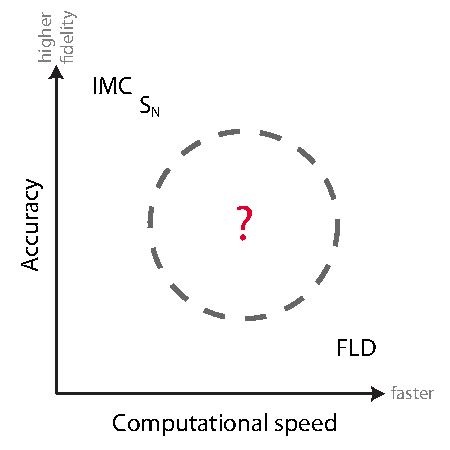
\includegraphics[width=3in]{fidelity}
  \caption{Figurative representation of existing TRT methods, showing the
  trade-off between accuracy and speed.}
  \label{fig:fidelity}
\end{figure}

With our development of anisotropic diffusion and its application to TRT, we
hope to provide a new solution process that is much less expensive than
full-fledged transport but more theoretically robust than standard diffusion or
FLD. Such a method would fit near the question mark in
Fig.~\ref{fig:fidelity}.

%%%%%%%%%%%%%%%%%%%%%%%%%%%%%%%%%%%%%%%%%%%%%%%%%%%%%%%%%%%%%%%%%%%%%%%%%%%%%%%%
\section{Synopsis}

The remainder of this thesis is organized into the following chapters.

\chaptersynopsis{chap:trtBackground}
The assertions about the difficulty of computational modeling of thermal
radiative transfer are explained by presenting the equations themselves. We give
a brief overview of existing approximations to the TRT equations and discuss how
those approximations are used in our work. Particular emphasis is given to the
semi-implicit treatment, which allows the nonlinear problem to be approximated
by a system of linear equations.

\chaptersynopsis{chap:adDerivation}
With the transport equation in hand, we derive a new approximation to radiation
transport, anisotropic diffusion. The derivation accounts for both time
dependence and boundary conditions. We then discuss some of the properties of
the AD method and make predictions for its range of applicability.

\chaptersynopsis{chap:aponeDerivation}
The derivation of the time-dependent AD equations assumed that the solution
changes slowly in time, which can be a poor approximation when applied to
TRT: it can actually lead to the nonphysical transfer of energy faster than the
speed of
light. This chapter addresses that shortcoming by modifying the ansatz used in
deriving the anisotropic diffusion equations, leading to a new ``anisotropic
\Pone'' method.

\chaptersynopsis{chap:implementation}
The leakage terms for anisotropic diffusion are more complex than standard
diffusion: rather than a scalar diffusion coefficient, AD has a diffusion
tensor. This necessitates unusual discretization schemes in all but the simplest
of problems. We present new discretization schemes for Cartesian \xy\ geometry
that can account for the transverse leakage induced by the anisotropic diffusion
tensor.

\chaptersynopsis{chap:flatland}
As mentioned earlier, the ``flatland'' geometry has recently proven to be a
valuable test bed for new transport methods because of its smaller phase space
and correspondingly easier solution. This chapter gives a thorough overview of
the differences between flatland and true 3-D geometries, with a focus on
implementing flatland solvers. We also explore diffusion in flatland, not only
deriving the prior result that the diffusion coefficient is different but also
formulating correct diffusion boundary conditions. Finally, we present the AD
equations in flatland geometry.

\chaptersynopsis{chap:simpleNumericalResults}
Before applying the anisotropic approximations to full nonlinear transport in
multi-dimensional geometries, it is important that we test individual components
of the derivation. We detail several steady-state problems that test the
discretization schemes, flatland diffusion boundary conditions, and anisotropic
diffusion boundary conditions. We also test some simple linear transport
problems.

\chaptersynopsis{chap:trtNumericalResults}
Finally, we test the applicability of the anisotropic methods to the nonlinear
TRT equations. To begin, we examine a few simple test problems in 1-D, where the
anisotropic methods merely ``smear'' the diffusion coefficients spatially.
This provides a test bed for determining the robustness of the nonlinear
treatment. Then
we move to more complicated flatland problems that simulate radiation flow
through an optically thin channel. (This is the qualitative configuration of
the CRASH problem.)
Additionally, we apply the AD method to some difficult 2-D problems in the
literature that feature optically thick obstacles rather than optically thin
streaming channels.

\chaptersynopsis{chap:conclusion}
The final chapter summarizes the results of the theory developed in this thesis
and its application to TRT problems. We discuss possible improvements to the new
methods and other future work.


% !TEX root = _individual/trtBackground.tex

%%%%%%%%%%%%%%%%%%%%%%%%%%%%%%%%%%%%%%%%%%%%%%%%%%%%%%%%%%%%%%%%%%%%%%%%%%%%%%%%
\chapter{Background to Thermal Radiative Transfer}\label{chap:trtBackground}

In order to elucidate the derivation and application of the anisotropic
diffusion approximation, it is necessary to delve deeper into the physical
process that is subject to the approximation. As discussed in the introduction,
thermal radiative transfer is the physical process of energy transfer via
high-energy photons in hot materials. Because the TRT equations and
approximations have been probed and reviewed in countless other works
\cite{Mih1984,Pom1973,Cas2004,Wol2008}, our aim is a concise explanation of the
physics relevant to the anisotropic diffusion approximation and its immediate
application, rather than a thorough overview of the extensive field of radiation
hydrodynamics. We also review the derivation of competing solution methods and
discuss their advantages and shortcomings.

%%%%%%%%%%%%%%%%%%%%%%%%%%%%%%%%%%%%%%%%%%%%%%%%%%%%%%%%%%%%%%%%%%%%%%%%%%%%%%%%
\section{Equations of transfer}\label{sec:bgTrtEquations}
Thermal radiative transfer describes how high-energy photons move energy about
in a very hot material, such as the interior of a star or the target of a laser
fusion experiment. The equations that model TRT are time-dependent, contain
strong nonlinearities, and reside in a large phase space.
A full representation of the physics in
the high-energy-density regime often includes the consideration of moving
relativistic materials, different electron and ion temperatures, photon
scattering, and thermal conduction in the material \cite{Mih1984}. However,
much theoretical work in the field neglects these complex phenomena by
\begin{itemize}
  \item working in a fixed medium, disregarding material advection;
  \item assuming local thermodynamic equilibrium (LTE), which uses a single
    material temperature;
  \item neglecting photon scattering, which tends to be comparatively small for
    very hot materials; and
  \item neglecting thermal conduction, since energy transfer is dominated by
    radiation in the temperature regimes we consider.
\end{itemize}

A further simplification often used for methods development is the ``gray''
approximation to the frequency dependence. Analogous to the one-group
approximation for neutron transport, the full transport equation is integrated
over all frequencies, and the opacities are averaged with some \emph{a priori}
weighting function, typically the Rosseland mean \cite{Lar1983a}.

For the purposes of discussion and the later AD derivation, we consider a
general, 3-D universe, where the spatial coordinates are
\begin{equation*}
  \vec{x}
  = x \vec{i} + y \vec{j} + z \vec{k}\,,
\end{equation*}
and the angular coordinates are the unit vector
\begin{equation*}
  \vec{\Omega}
  = \mu \vec{i}
  + \sqrt{1-\mu^2} \cos \theta \vec{j}
  + \sqrt{1-\mu^2} \sin \theta \vec{k} \,.
\end{equation*}
These angular coordinates reside in the domain $-1 \le \mu \le 1$, $0 \le \theta
< \pi$; we use $\vec{\Omega}\in4\pi$ as a frequent shorthand denoting the entire
unit sphere. See \cite{Lar2007,Pri2010} for a more complete discussion of the
spatial and angular coordinate systems.

After the simplifications described above, the thermal radiative transfer
process in the interior of a problem (away from the initial time and
from boundaries) can be described \cite{Pom1973} by
\begin{subequations} \label{eqs:explanTRT}
the radiative transfer equation,
\begin{equation} \label{eq:explanTransport}
  \frac{1}{c} \pder{I}{t}
  + \vec{\Omega} \vd \del I +
 \sigma I
  = \frac{\sigma a c T^4}{4\pi} 
  + \frac{c q_r}{4\pi} \,,
\end{equation}
and the material energy balance equation,
\begin{equation} \label{eq:explanMaterial}
  c_v \pder{T}{t} = \sigma \int_{4\pi}  I \ud \Omega - \sigma a c T^4 \,.
\end{equation}
\end{subequations}

The notation and omitted parameters in Eqs.~\eqref{eqs:explanTRT} are:
\begin{alignat*}{2}
  I &= I(\vec{x}, \vec{\Omega}, t) &&= \text{the angular
  radiation intensity,}
  \\
  T &= T(\vec{x}, t) &&= \text{the material temperature,}
  \\
  \sigma &= \sigma(\vec{x}, T) &&= \text{the absorption opacity,} 
  \\
  q_r &= q_r(\vec{x}, t) &&= \text{an extraneous isotropic radiation energy source,}
  \\
  c_v &= c_v(\vec{x}, T) &&= \text{the specific heat capacity of a material,}
  \\
  a& &&= \text{the radiation constant, and}
  \\
  c& &&= \text{the speed of light.}
\end{alignat*}
The intensity $I$ and the temperature $T$ are the primary unknowns: they
describe the state of energy in the radiation and in the material.
Each of the terms that depends on $T$ implicitly depends on the time $t$. The
explicit dependence of $c_v$ and $\sigma$ on $\vec{x}$ accounts for different
materials in different parts of the problem.

Equation~\eqref{eq:explanTransport} is a transport equation for $I$. The first
two terms describe how photons ``stream'' in time and space: if the $\sigma$
and source terms were zero, Eq.~\eqref{eq:explanTransport} would reduce to a
wave equation with a wave speed of $c$. However, because the photons are moving
through a material, there is a chance they will collide with the material,
hence the \emph{collision} term $\sigma I$. The first term on the right-hand
side represents particles emitted via the isotropic temperature-dependent
process of black body emission. The additional term $q_r$ is an extraneous
isotropic radiation source that emits with an energy density (energy per
volume per time) of $q_r$.

The material equation~\eqref{eq:explanMaterial} describes an energy balance in
the material. On the left-hand side is the time rate of change in the material
energy density, which is a function of the material's temperature and specific
heat capacity $c_v$:
\begin{equation} \label{eq:matEnergyDens}
  U_m(T) = \int_{0}^{T} c_v(T') \ud T' \,.
\end{equation}
The first term on the right hand side exactly mirrors the collision term in the
radiation equation: it is a ``gain'' term corresponding to photons that
collided with (were absorbed by) the material. The second term describes when
energy is lost from the material and emitted as radiation: black body emission.

In order to conserve energy in a simulation, strict attention must be paid to
$U_m$ and $\phi$, which are the true quantities of energy in
the material and radiation. If the loss, gain, and rate of change terms are not
properly treated, energy will not be conserved.

The physical properties $\sigma$ and $c_v$ are often approximated by simplistic
models in the methods development sphere. The heat capacity $c_v$ of an ideal
gas is a constant, giving the material energy $U_m$ a linear proportionality to
the material temperature $T$. A much-used model \cite{Mou2006,Wol2008} of the
gray opacity is $\sigma \propto \propto T^{-3}$.
Our numerical test problems will use both of these idealized representations of
the physical constants.

The nonlinear coupling between Eqs.~\eqref{eq:explanTransport}
and~\eqref{eq:explanMaterial} via $T^4$ emission and $T^{-3}$ absorption make
the TRT equations extremely ``stiff'' \cite{Kno2003} and therefore even more
difficult to solve than the standard linear transport equation. In this work,
we will not attempt to provide any new solutions to treat the nonlinearities,
but we will formulate our time-dependent anisotropic diffusion approximations to
be compatible with multiple solution techniques.

\subsection{The radiation intensity}

In radiative transfer, the intensity $I$ is the energy-weighted radiation path
length density, similar to the angular flux $\psi$ in reactor physics:
\begin{equation*}
  I(\vec{x},\vec{\Omega},\nu, t) = c h\nu N(\vec{x},\vec{\Omega},\nu, t)\,,
\end{equation*}
where $h\nu$ is the photon energy and $N$ is the photon density,
\begin{align*}
  N(\vec{x},\vec{\Omega}, \nu, t) \ud V \ud \Omega
  &= \topbox{the number of photons inside the differential volume $\ud V$
  about $\vec{x}$, traveling in the directions $\Omega$ about
  $\vec{\Omega}$, inside the frequencies $\ud \nu$ about $\nu$, at time $t$.}
\end{align*}
Integrating over all energy gives the gray intensity,
\begin{equation*}
  I(\vec{x},\vec{\Omega}, t)
  = c \int_0^\infty h\nu N(\vec{x},\vec{\Omega},\nu, t) \ud\nu \,.
\end{equation*}

Additionally, integrating over all angles (i.e.~taking the zeroth angular
moment) yields the ``scalar intensity''
\begin{align} \label{eq:intensityZeroth}
  \phi(\vec{x},t) &\equiv \int_{4\pi} I(\vec{x},\vec{\Omega}, t) \ud \Omega
  \\
  &= c \int_{4\pi} \int_0^\infty h\nu N(\vec{x},\vec{\Omega},\nu, t) \ud\nu
   \ud \Omega
\\ \intertext{which is directly proportional to the radiation energy density:}
\nonumber
\frac{1}{c} \phi(\vec{x},t) \ud V
&= \topbox{the amount of energy in the radiation field inside the differential
  volume $\ud V$ about $\vec{x}$, at time $t$.}
\end{align}
For our work, it is usually more convenient to refer to $\phi$ than to the
radiation energy density (compare, for example, \cite{Den2007} to
\cite{Kno1999a}). In fact, since in our computational experiments we use the
scaled system of variables $c=a=1$, our later results can use ``scalar
intensity'' and ``radiation energy density'' interchangeably.

The first angular moment of the intensity also has physical significance. The
radiation flux is defined as
\begin{equation} \label{eq:intensityFirst}
  \vec{F}(\vec{x},t) \equiv \int_{4\pi} \vec{\Omega}
  I(\vec{x},\vec{\Omega}, t) \ud \Omega \,.
\end{equation}
Analogous to the ``neutron current'' $\vec{J}$ in reactor physics, the
radiation flux is the net rate of energy flowing through a point.

At any particular point in space and time, the radiation intensity $I$ is
generally a complicated function of angle.%
\footnote{See \cite{Ada2001a} for an example of how complicated a function of
angle the transport solution can be in even a simple reactor physics problem.}
For example, at the edge of a
radiation shock wave, the distribution is highly peaked in the directions
pointed away from the hot region, because that is the source of the photons. In
other parts of the problem where the system is closer to an equilibrium state,
the intensity is nearly isotropic: that is, the intensity is almost a uniform
function in angle.

%%%%%%%%%%%%%%%%%%%%%%%%%%%%%%%%%%%%%%%%%%%%%%%%%%%%%%%%%%%%%%%%%%%%%%%%%%%%%%%%
\section{Semi-implicit linearization}\label{sec:bgSemiImplicit}

The anisotropic diffusion approximation is intended for use in a deterministic
manner. It is therefore necessary to discuss \emph{discretization} schemes,
where the continuous unknowns in Eqs.~\eqref{eqs:explanTRT} are approximated
with discrete unknowns. In this section, we tackle the discretization of the
time variable in the context of \emph{linearization}, where the nonlinear
aspects of the TRT equations are approximated to allow a linear algebraic
representation of the system of unknowns, facilitating their solution on a
computer.

To solve the TRT equations with deterministic methods, we use the common
``semi-implicit'' scheme \cite{Kno1999a,Kno2001,Low2004}, where operator splitting
is used to decouple the radiation and material equations inside a time step, and
a backward Euler discretization is used with the unknowns.
Like Fleck and Cummings' IMC method \cite{Fle1971}, this technique
yields a linear transport equation with a pseudo-scattering term. Because of the
extensive use of this
nonlinear treatment in our implementations of anisotropic diffusion and the
other tested methods, and because the semi-implicit scheme for radiation
transport is usually glossed over or presented vaguely in other works, we derive
it here in some level of detail.

For the semi-implicit discretization, it is more convenient to write
Eqs.~\eqref{eqs:explanTRT} in a slightly altered form:
\begin{subequations} \label{eqs:semiTRT}
\begin{equation} \label{eq:semiTransport}
  \frac{1}{c} \pder{I}{t}
  + \vec{\Omega} \vd \del I +
 \sigma I
 = \frac{\sigma c U_r}{4\pi} 
  + \frac{c q_r}{4\pi} \,,
\end{equation}
and the material energy balance equation,
\begin{equation} \label{eq:semiMaterial}
  \pder{U_m}{t} = \sigma \int_{4\pi}  I \ud \Omega - \sigma c U_r \,.
\end{equation}
\end{subequations}
Here, we have defined the ``equilibrium radiation energy density'' of a
material as a scaled integral of the Planckian emission function:
\begin{equation} \label{eq:radEnergyDens}
  U_r(T) \equiv aT^4
  = \frac{1}{c} \int_{4\pi} \int_{0}^{\infty} B(\nu, T) \ud\nu \ud\Omega \,.
\end{equation}
Its physical relevance is that, when the radiation field and material reach
an equilibrium, $I=B$, and the radiation energy density $\phi/c$ is equal to
$U_r$.  The quantity $U_r$ is \emph{not} equal to the energy density stored in
the material, $U_m$.

\subsection{Linearizing the material energy equation}

First, we define a parameter $\beta$ as a function of
Eqs.~\eqref{eq:matEnergyDens} and~\eqref{eq:radEnergyDens}:
\begin{equation} \label{eq:beta}
  \beta(\vec{x}, T) \equiv \pder{U_r}{U_m} 
  = \pder{U_r}{T} \Bigg/ \pder{U_m}{T}
  = \frac{4 a T^3}{c_v(\vec{x}, T)} \,.
\end{equation}
The chain rule allows the left hand side of Eq.~\eqref{eq:semiMaterial} to be
expressed without approximation in terms of the equilibrium radiation energy
density $U_r$:
\begin{equation*}
  \pder{U_m}{t} = \pder{U_m}{U_r} \pder{U_r}{t} = \frac{1}{\beta(T)}
  \pder{U_r}{t} = \sigma \int_{4\pi}  I \ud \Omega - \sigma c U_r \,.
\end{equation*}
The first approximation is to ``freeze'' the parameter $\beta$ at the beginning-of-time-step temperature $T^n$:
\begin{equation}\label{eq:frozenBeta}
  \frac{1}{\beta^n}
  \pder{U_r}{t} \approx \sigma \int_{4\pi}  I \ud \Omega - \sigma c U_r \,.
\end{equation}
The process of freezing $\beta$ is equivalent to approximating the
Planckian emission term with a Taylor series \cite{Kno2007}.

Because the approximation to $\beta$ is an approximation to the rate of change
in material energy, this equation no longer conserves the system's total
energy. To enforce conservation of energy over a time step, we must set the
material energy change over a time step to the time-integrated approximation:
\begin{align}
  \nonumber
  \int_{t^n}^{t^{n+1}}  \pder{U_m}{t}\ud t &= \frac{1}{\beta^n}
  \int_{t^n}^{t^{n+1}} \pder{U_r}{t}\ud t
  \\
  \nonumber
  U_m^{n+1} - U_m^n &= \frac{1}{\beta^n} \left[ U_r^{n+1} - U_r^n \right]
  \\
  \label{eq:matenConservationUpdate}
  U_m^{n+1} &=  U_m^n + \frac{U_r^{n+1} - U_r^n}{\beta^n}\,.
\end{align}
%Thus, the expression of $\tpder{U_m}{t}$ in terms of $\tpder{U_r}{t}$

The next approximation is to explicitly freeze the opacity $\sigma$ in
Eq.~\eqref{eq:frozenBeta}:
\begin{equation*}
  \frac{1}{\beta^n}
  \pder{U_r}{t} \approx \sigma^n \int_{4\pi}  I \ud \Omega - \sigma^n c U_r \,.
\end{equation*}
Now we can time-average the material equation to express it in terms of two
simple time-average unknowns. Operating by
$\frac{1}{\Delta_t^n}\int_{t_n}^{t^{n+1}} (\cdot) \ud t$,
\begin{equation*}
  \frac{1}{\beta^n}
  \frac{U_r^{n+1} - U_r^n}{\Delta_t^n} = \sigma^n \int_{4\pi} \left[
  \frac{1}{\Delta_t^n}\int_{t_n}^{t^{n+1}} I\ud t
  \right] \ud \Omega - \sigma^n c \left[
  \frac{1}{\Delta_t^n}\int_{t_n}^{t^{n+1}} U_r \ud t \right]\,.
\end{equation*}
Next, we apply the implicit Euler approximation%
\footnote{Note that the IMC method only applies the implicit approximation to
$U_r$, allowing the continuous-in-time treatment of $I$.}%
to $U_r(\vec{x}, \vec{\Omega}, t)$ and $I(\vec{x}, \vec{\Omega}, t)$ by setting
their time-averaged values to
the values at $t^{n+1}$:
\begin{equation} \label{eq:semiImplicitMaterial}
  \frac{1}{\beta^n(\vec{x})}
  \frac{U_r^{n+1}(\vec{x}) - U_r^n(\vec{x})}{\Delta_t^n}
  = \sigma^n(\vec{x}) \int_{4\pi} I^{n+1}(\vec{x}, \vec{\Omega})\ud \Omega
  - c \sigma^n(\vec{x}) U_r^{n+1}(\vec{x}) \,.
\end{equation}

We solve Eq.~\eqref{eq:semiImplicitMaterial} for $U_r^{n+1}$ in order to
eliminate the implicit dependence of the transport equation on the material
energy equation.
\begin{align} \nonumber
  U_r^{n+1} [ 1 + c \beta^n \Delta_t^n \sigma^n ]
  &= \beta^n \Delta_t^n \sigma^n\int_{4\pi} I^{n+1}\ud \Omega + U_r^n
   \\ \nonumber
  U_r^{n+1}
  &= \frac1c \frac{ c \beta^n \Delta_t^n \sigma^n }{ 1 + c \beta^n \Delta_t^n \sigma^n}
  \int_{4\pi} I^{n+1}\ud \Omega + \frac1{ 1 + c \beta^n \Delta_t^n \sigma^n}
  U_r^n
  \\ \label{eq:urNPlusOne}
  U_r^{n+1}
  &= \left(1 - f^n\right) \frac1c \int_{4\pi} I^{n+1}\ud \Omega + f^n U_r^n
\end{align}
where we have defined the Fleck factor \cite{Fle1971} as
\begin{equation} \label{eq:fleckFactor}
  f^n = f^n(\vec{x}) \equiv \left[ 1 + \beta^n c \Delta_t^n \sigma^n
  \right]\inv \,.
\end{equation}

\subsection{Linearizing the transport equation}
The next step is apply similar approximations to the nonlinear radiation
transport equation~\eqref{eq:semiTransport}. As with the material equation,
the
opacities are ``frozen'' at their beginning-of-time-step values $\sigma^n$, and
the equation is time-averaged:
\begin{multline*}
  \frac{1}{c} \frac{I^{n+1} - I^n}{\Delta_t^n}
  + \vec{\Omega} \vd \del \left[
  \frac{1}{\Delta_t^n}\int_{t_n}^{t^{n+1}} I\ud t
  \right] +
 \sigma^n \left[
  \frac{1}{\Delta_t^n}\int_{t_n}^{t^{n+1}} I\ud t
  \right]
  \\
  = \frac{\sigma^n c}{4\pi} \left[
  \frac{1}{\Delta_t^n}\int_{t_n}^{t^{n+1}} U_r \ud t \right]
  + \frac{1}{4\pi}\left[
  \frac{1}{\Delta_t^n}\int_{t_n}^{t^{n+1}} q_r \ud t \right] \,.
\end{multline*}
Since the extraneous energy source $q_r$ is assumed to be known \emph{a priori},
we let its time-averaged value be $q_r^n$. As in the material equation, we apply
the implicit Euler approximation to $I$ and $U_r$:
\begin{equation*}
  \frac{1}{c} \frac{I^{n+1} - I^n}{\Delta_t^n}
  + \vec{\Omega} \vd \del I^{n+1}
 + \sigma^n I^{n+1}
 = \frac{\sigma^n c}{4\pi} U_r^{n+1}
  + \frac{c}{4\pi} q_r^n \,.
\end{equation*}
Finally, we substitute $U_r^{n+1}$ from Eq.~\eqref{eq:urNPlusOne},
which was derived from the material equation Eq.~\eqref{eq:semiMaterial}:
\begin{align}\nonumber
  \frac{1}{c} \frac{I^{n+1} - I^n}{\Delta_t^n}
  + \vec{\Omega} \vd \del I^{n+1}
 + \sigma^n I^{n+1}
 &= \frac{\sigma^n c}{4\pi} \left[ \left(1 - f^n\right) \frac1c \int_{4\pi} I^{n+1}\ud \Omega + f^n U_r^n \right]
  + \frac{c}{4\pi} q_r^n
  \\ \label{eq:linearizedGrayTransport}
  \frac{1}{c} \frac{I^{n+1} - I^n}{\Delta_t^n}
  + \vec{\Omega} \vd \del I^{n+1}
 + \sigma^n I^{n+1}
 &=  \left(1 - f^n\right) \sigma^n \frac{1}{4\pi} \int_{4\pi} I^{n+1}\ud \Omega
 + \frac{1}{4\pi} f^n \sigma^n c U_r^n
  + \frac{1}{4\pi} c q_r^n \,.
\end{align}

\subsection{Comments}\label{bgSIComments}
If we compare Eq.~\eqref{eq:linearizedGrayTransport} to a temporally implicit
discretization of a monoenergetic linear transport problem with isotropic
scattering,
\begin{equation*}
  \frac{1}{v} \frac{\psi^{n+1} - \psi^n}{\Delta_t^n} 
  + \vec{\Omega} \vd \del \psi^{n+1}
 + \Sigma_t \psi^{n+1}
 = \frac{1}{4\pi} \int_{4\pi} \psi^{n+1}\ud \Omega
  + \frac{1}{4\pi} q \,,
\end{equation*}
we find equivalences between the two:
\begin{alignat*}{2}
  I &\leftrightarrow \psi &&= \text{the angular flux,}
  \\
  \sigma^n &\leftrightarrow \Sigma_t &&= \text{the total cross section,}
  \\
  \left(1 - f^n\right) \sigma^n &\leftrightarrow \Sigma_s &&= \text{the scattering cross
  section,} 
  \\
  f^n \sigma^n c U_r^n + c q_r^n &\leftrightarrow q &&= \text{the isotropic source for time
  step $n$,}
  \\
  v   &\leftrightarrow c &&= \text{the particle velocity.}
\end{alignat*}
Even though the original radiation transport equation was purely
absorbing, the linearization scheme created a ``pseudoscattering''
term that essentially emulates the absorption and isotropic re\"emission of
radiation during a time step. The IMC literature often refers to the
``effective scattering opacity,''
$\sigma_\text{es}^n \equiv \left(1 - f^n\right) \sigma^n$.

Furthermore, if we take the zeroth angular moment of
Eq.~\eqref{eq:linearizedGrayTransport} and let $\phi^{n+1}(\vec{x}) \equiv
\frac{1}{4\pi} \int_{4\pi} I^{n+1}\ud \Omega$, then we find the radiation
energy conservation equation over the time step to be
\begin{equation}\label{eq:semiImplicitZeroth}
  \frac{1}{c} \frac{\phi^{n+1} - \phi^n}{\Delta_t^n}
  + \del \vd \vec{F}^{n+1} + f^n\sigma^n \phi^{n+1}
 =  f^n \sigma^n c U_r^n + c q_r^n\,.
\end{equation}
The quantity, $\sigma_\text{ea}^n \equiv f^n\sigma^n$ is known as the
``effective absorption opacity.''

\subsection{Solution process summary}
The time-dependent radiation solution is stored in the linear time-dependent
transport solver. The material energy $U_m$ must be stored, but the
material temperature can be either stored (highly recommended because of its
frequent use) or calculated on the fly from $U_m$ by inverting the integral in
Eq.~\eqref{eq:matEnergyDens}.

For the $n$th time step, given the initial radiation field $I^{n}$ and the
initial material energy density $U_m^n$, the solution process follows.
\begin{enumerate}
  \item \emph{Linearize the system.} Using the starting temperature $T^n$,
    calculate
    the frozen $\sigma^n$ and $\beta^n$ in each spatial cell. Use
    Eq.~\eqref{eq:fleckFactor} to calculate $f^n$, which in turn is used to
    calculate the linearized isotropic source $f^n \sigma^n c U_r^n + c q_r^n$
    and the effective scattering cross section $\left(1 - f^n\right) \sigma^n$.
    If using a diffusion method to approximate the transport solution, the
    absorption cross sections and diffusion coefficients must be recalculated.

  \item \emph{Solve the linear transport problem for $\psi^{n+1}=I^{n+1}$.} The new
    radiation
    temperature can optionally be calculated:
    \begin{equation*}
      a (T_\text{rad}^{n+1})^4 = \frac{1}{c} \int_{4\pi} I^{n+1}
      \ud \Omega
      \lra
      T_\text{rad}^{n+1}(\vec{x})
      = \left[ \frac{\phi^{n+1}(\vec{x})}{ac} \right]^{1/4}\,.
    \end{equation*}

  \item \emph{Update the material temperature.} From Eq.~\eqref{eq:urNPlusOne}
    we can calculate the linearized estimate of $U_r^{n+1}$:
    \begin{equation*}
      U_r^{n+1} = \left(1 - f^n\right) \frac1c \phi^{n+1}  + f^n U_r^n\,.
    \end{equation*}
    However, because of the linearization of $\beta$, $U_r^{n+1} \ne a
    (T^{n+1})^4$. Instead, to calculate the material temperature, we must use
    Eq.~\eqref{eq:matenConservationUpdate}. Substituting
    Eq.~\eqref{eq:urNPlusOne} into Eq.~\eqref{eq:matenConservationUpdate}
    and simplifying gives
    \begin{equation}\label{eq:matenConservationUpdate2}
      U_m^{n+1} = U_m^n + f^n \sigma^n \Delta_t^n
      \left[ \phi^{n+1} - c U_r^n \right] \,.
    \end{equation}
    [This form can also be derived by integrating
    Eq.~\eqref{eq:semiMaterial} over a time step after making the
    approximation $\sigma(T) \approx \sigma(T^n)$.]
\end{enumerate}

Figure~\ref{fig:semiImplicitFlowchart} shows how the quantities $\Delta_t$,
$\beta$, $\sigma$, $f$, etc.~relate. This relation is especially important when
implementing the linearization scheme programmatically. 

\begin{sidewaysfigure}[hp]
  \centering
  \includegraphics[width=8in]{semi-implicit}
  \caption{Dependency graph of quantities in the semi-implicit discretization.}
  \label{fig:semiImplicitFlowchart}
\end{sidewaysfigure}

%%%%%%%%%%%%%%%%%%%%%%%%%%%%%%%%%%%%%%%%%%%%%%%%%%%%%%%%%%%%%%%%%%%%%%%%%%%%%%%%
\clearpage
\section{Deterministic radiation transport approximations}
\label{sec:bgApproxMethods}

In this section, we briefly review several existing deterministic radiation transport methods.

The salient difference among these methods is in their treatment of
the angular dependence of the solution. Additionally, each method tends to have
its own set of spatial discretizations that are effective and efficient for the
given angular treatment. The choice of temporal discretization is usually
independent of the method used. Every approximation applied to the transport
equation introduces a source of error.

Approximations to the angular behavior of $I$ introduce definite errors
that are often surprisingly hard to quantify. Asymptotic analysis can be used to
describe quantitative regimes of applicability, but we will confine our
discussion to some of the qualitative unphysical behavior introduced by the
angular approximations.

Innumerable spatial discretizations exist. Typically, a
spatial discretization will introduce a local error into the solution in some
relation to the grid size. In the diffusion (and anisotropic diffusion) methods,
the most convenient methods to use are often finite difference schemes
\cite{Lev2007}. It should also be noted for the sake of completion that for more
complex angular approximations than diffusion such as \SN, the grid error is not
the most serious problem; poor asymptotic behavior for optically
thick cells can lead to highly inaccurate answers \cite{Ada1998a,Ada2001}.

Finally, the treatment of the time dependence of the TRT equations is a lengthy
topic \cite{Low2004}. As in other partial differential equations, the
approximation made to the
$\tpder{I}{t}$ term (or to the time average of the other terms) incurs a
discretization error of $O(\Delta_t)$ in the case of forward and backward Euler,
or $O(\Delta_t^2)$ and higher in other high-order discretization schemes.
Because of the stiff nature of the TRT equations \cite{Kno2003}, unstable explicit
methods such as forward Euler are practically unusable in this application.
Furthermore, the operator split in the semi-implicit treatment produces an
$O(\Delta_t)$ linearization error. Typically, then,
higher-order methods require iteration on the nonlinearities or the
application of Jacobi-free Newton--Krylov techniques. In our work, we will use
only the simple semi-implicit linearization with the backward Euler implicit time
discretization, so our discussion of the methods in this section will represent
the transport equation in the linearized form
\begin{equation}\label{eq:siTransport}
  \frac{1}{c} \frac{I^{n+1} - I^n}{\Delta_t^n}
  + \vec{\Omega} \vd \del I^{n+1}
  + \sigma^n I^{n+1}
  = \frac{1}{4\pi} \sigma_\mathrm{es}^n \phi^{n+1}
  + \frac{1}{4\pi} Q^n\,.
\end{equation}

%%%%%%%%%%%%%%%%%%%%%%%%%%%%%%%%%%%%%%%%
\subsection{Discrete ordinates}

The discrete ordinates (\SN) method approximates the angular dependence of the
intensity with a quadrature set of $M$ angles $\vec{\Omega}_m$ with weights $w_m$:
\begin{equation*}
  I(\vec{x},\vec{\Omega},t) \approx \sum_{m=1}^M I_m(\vec{x},t) \vec{\Omega}_m w_m\,.
\end{equation*}
Applying the angular approximation to Eq.~\eqref{eq:siTransport}, we get $N$
equations 
\begin{equation}\label{eq:siTransport}
  \frac{I_{m}^{n+1} - I_{m}^n}{c \Delta_t^n}
  + \vec{\Omega}_{m} \vd \del I_{m}^{n+1}
  + \sigma^n I^{n+1}
  = \frac{1}{4\pi} \sigma_\mathrm{es}^n \phi^{n+1}
  + \frac{1}{4\pi} Q^n\,.
\end{equation}
The equations for each equation are coupled at every point in space through the
scalar intensity in the scattering term:
\begin{equation*}
  \phi^{n+1} = \sum_{m=1}^M I_m^{n+1} w_m \,.
\end{equation*}
The equations can also be coupled at the boundaries of a problem, e.g.~via
specular reflection.

To interpret Eq.~\eqref{eq:siTransport} as a linear algebraic expression, we
rearrange it slightly:
\begin{equation*}
  \left( \vec{\Omega}_{m} \vd \del + \frac{1}{c\Delta_t^n}
  + \sigma^n \right) I_{m}^{n+1}
  = \frac{1}{c\Delta_t^n} I_{m}^n
  + \frac{1}{4\pi} \sigma_\mathrm{es}^n \phi^{n+1}
  + \frac{1}{4\pi} Q^n
\end{equation*}
or, combining all $M$ equations into abstract linear operators (similar to
\cite{War2004}),
\begin{equation*}
  L \psi = S \psi + q\,,
\end{equation*}
where $L$ is the operator representing ``streaming plus collision'' on the left
hand side, $S$ represents the isotropic redistribution of photons via
scattering, $\psi$ is the vector of unknown angular intensity at the new time
step, and $q$ is the isotropic source plus the initial condition. At every time
step, the \SN\ equations are typically solved iteratively with Richardson
iteration (or ``source iteration'') \cite{Lew1984},
\begin{equation*}
  \psi^{(k+1)} = L\inv ( S \psi^{(k)} + q )\,.
\end{equation*}
Every application of $L\inv$ to the unknowns is known as a ``transport sweep,''
as it normally implemented not as an explicit matrix of unknowns but rather in
an algorithm that sweeps across a mesh, progressively solving the transport
equation in each cell.
In the absence of scattering ($\sigma_\mathrm{es}^n=0$) and without boundaries,
the \SN\ equations can be solved in only one sweep, which is particularly
advantageous for the anisotropic diffusion solution process.

In highly scattering systems, \SN\ can take an arbitrarily long time to converge
using pure source iteration. Means of overcoming this, including diffusion
synthetic acceleration, multigrid treatments, and Krylov methods, are well
outside the scope of this background chapter. Our primary use of the \SN\ method
as presented here is to visualize the angular dependence of the intensity at
different points in space-time.

%%%%%%%%%%%%%%%%%%%%%%%%%%%%%%%%%%%%%%%%
\subsection{Spherical harmonics}\label{sec:bgPn}
The spherical harmonics (\PN) method takes a very different approach to
approximating the angular dependence of the intensity. It expresses the
intensity as a truncated series of angular moments,
\begin{align*}
  I(\vec{x},\vec{\Omega},t)
  &\approx \sum_{l=0}^{L} \sum_{m=-l}^{l} Y_{l,m}(\vec{\Omega}) \left[
  \int_{4\pi} Y_{l,m}^\ast(\vec{\Omega}') I(\vec{x},\vec{\Omega}',t) \ud \Omega'
  \right]
  \\
  &= \frac{1}{4\pi} \phi(\vec{x}, t) + \frac{3}{4\pi} \vec{\Omega}\vd
  \vec{F}(\vec{x},t) + \cdots\,,
\end{align*}
where $Y_{l,m}(\vec{\Omega})$ and $Y_{l,m}^*(\vec{\Omega})$ are the spherical
harmonic functions and their complex conjugates \cite{McC2008a,Lar2007}.

The full spherical harmonic equations \cite{McC2007} are lengthy, complicated, and
largely irrelevant to our work. However, the \Pone\ equations, which result from
taking $L=1$, are relevant. The first step in their derivation is to take the
zeroth and first angular moments of Eq.~\eqref{eq:siTransport}. The zeroth
angular moment of the linearized transport equation is
\begin{equation}\label{eq:p1ZerothMoment}
  \frac{\phi^{n+1} - \phi^n }{c \Delta_t}
  + \grad \vd \vec{F}
  + \sigma_\mathrm{ea}^n \phi^{n+1}
  = Q^n\,,
\end{equation}
and the first moment is the vector equation
\begin{equation}\label{eq:p1FirstMoment}
  \frac{\vec{F}^{n+1} - \vec{F}^n }{c \Delta_t} + \grad \vd \int_{4\pi}
  \vec{\Omega}\vec{\Omega} I^{n+1} \ud\Omega
  + \sigma^n \vec{F}^{n+1}
  = 0\,.
\end{equation}

The \Pone\ approximation provides a closure for Eq.~\eqref{eq:p1FirstMoment} by
approximating the intensity as
\begin{equation}\label{eq:p1Approx}
  I^{n+1}(\vec{x},\vec{\Omega})
  \approx \frac{1}{4\pi} \phi^{n+1}(\vec{x})
  + \frac{3}{4\pi} \vec{\Omega}\vd \vec{F}^{n+1}(\vec{x}) \,,
\end{equation}
so the second angular moment is
\begin{equation*}
  \int_{4\pi} \vec{\Omega}\vec{\Omega} I^{n+1} \ud\Omega
  \approx \frac{1}{4\pi} \phi^{n+1}
  \int_{4\pi} \vec{\Omega}\vec{\Omega}\ud\Omega + 0
  = \frac{4\pi}{3} \Identitytens \phi^{n+1}\,,
\end{equation*}
where $\Identitytens$ is the identity matrix (the unit dyad). Thus
Eq.~\eqref{eq:p1FirstMoment} becomes
\begin{equation} \label{eq:p1FirstMoment2}
  \frac{\vec{F}^{n+1} - \vec{F}^n }{c \Delta_t} + \frac{1}{3} \grad \phi^{n+1}
  + \sigma^n \vec{F}^{n+1}
  = 0\,.
\end{equation}

Rather than the $M$ unknowns per spatial coordinate of the \SN\ method, the
\Pone has four (or, in 2-D space, three). It is therefore easier to solve and
store in computer memory. The disadvantages of \Pone\ are pronounced, however.
First, most obviously, the reduction in unknowns means the solution will almost
always lag in accuracy compared to a transport method. Second, it happens that
the approximation in Eq.~\eqref{eq:p1FirstMoment2} yields a plane wave
propagation speed of $c/\sqrt{3}$ rather than the physical $c$
\cite{Mih1984,War2002}. Even worse, the \Pone\ equation and in fact the entire
\PN\ family can produce negative solutions for $\phi^{n+1}$ in the presence of
steep gradients \cite{Bru2002,McC2007}. This is a particular problem in TRT
applications because a negative $\phi$ can lead to a negative temperature and
the catastrophic failure of a simulation.

An alternative to using the linear-in-angle approximation in the closure for
$\int_{4\pi} \vec{\Omega}\vec{\Omega} I^{n+1} \ud\Omega$ is to define an
Eddington tensor \cite{Pom1982,Ols2000} as
\begin{equation*}
  \Etens \equiv \frac{\int_{4\pi} \vec{\Omega}\vec{\Omega} I^{n+1}
  \ud\Omega}{\int_{4\pi} I^{n+1} \ud\Omega}\,,
\end{equation*}
so that Eq.~\eqref{eq:p1FirstMoment} becomes
\begin{equation*}
  \frac{\vec{F}^{n+1} - \vec{F}^n }{c \Delta_t}
  + \grad \vd \left( \Etens\phi^{n+1} \right)
  + \sigma^n \vec{F}^{n+1}
  = 0\,.
\end{equation*}
Typically, $\Etens$ is calculated via a transport problem or some \emph{a
priori} relation based on $\phi$ and its derivatives.
The variable Eddington factor, or quasidiffusion, family of methods can be much
more accurate than the \Pone\ equations, but the nonlinear closure for $\Etens$
can lead to nonphysical shocks and instabilities.

%%%%%%%%%%%%%%%%%%%%%%%%%%%%%%%%%%%%%%%%
\subsection{Diffusion}\label{sec:bgDiffusion}

After the \Pone\ approximation is applied to the first angular moment of the
transport equation, Eq.~\eqref{eq:p1Approx}, one further simplification leads to
the very common diffusion approximation. The ``quasi-static'' \cite{Dud1976}
approximation is to discard the time derivative term in
Eq.~\eqref{eq:p1FirstMoment}, simplifying the expression and allowing for an
explicit solution of $\vec{F}^{n+1}$ to yield Fick's law:
\begin{equation*}
  \vec{F}^{n+1} = - \frac{1}{3\sigma^n} \grad \phi^{n+1}\,.
\end{equation*}
This simple expression approximates the entire angular distribution of the
intensity $I$ with a single unknown, yielding a very small memory footprint and
typically very fast solution.

However, Fick's law is only a very coarse approximation, and it is not
necessarily accurate. An asymptotic analysis \cite{Lar1975,Lar1983a} shows that
the diffusion approximation actually is a leading
order solution of the transport equation given certain conditions---%
primarily, that the material properties vary slowly in space, and that the
system is highly scattering. For problems that have a fast time scale or have
strong absorbers, the diffusion approximation will not yield transport-quality
answers.

One particular property of the diffusion approximation in time-dependent
applications is that it yields a parabolic equation, allowing energy to be
transferred faster than the speed of light.

%%%%%%%%%%%%%%%%%%%%%%%%%%%%%%%%%%%%%%%%
\subsection{Flux-limited diffusion}\label{sec:bgFld}

The exact radiation intensity satisfies the mathematical identity $\norm{F} \le
\phi$,
essentially limiting the leakage of radiation at a point to the radiation
energy at that point. The identity can be proven using the triangle inequality:
\begin{align}
  \norm{\vec{F}} &= \norm{ \int_{4\pi} \vec{\Omega} I \ud \Omega}
  \\ \nonumber
  &\le \int_{4\pi} \norm{\vec{\Omega}} \abs{I} \ud \Omega 
  \\ \nonumber
  &\le \int_{4\pi} [1] I \ud\Omega
  \\ \nonumber
  \norm{\vec{F}} &\le \phi\,.
  \\ 
  \intertext{Substituting Fick's law for $\vec{F}$ gives a condition that the
  diffusion coefficient should ideally satisfy in the presence of large
  gradients:} \nonumber
  \norm{- D \grad \phi} &\le \phi
  \\ \label{eq:fluxLimit}
  D & \le \frac{\phi}{\norm{\grad \phi}} \,.
\end{align}
In a void, where $\sigma\approx 0$, this condition tends to be violated in
time-dependent problems.

A ``flux limiter'' is designed to combat this problem in an \emph{ad hoc} but
effective manner. Although certain flux limiters \cite{Lev1984} are based on
idealized forms that the radiation intensity might take where
Eq.~\eqref{eq:fluxLimit} tends to be violated, the usual approach is more
straightforward. The flux-limited diffusion (FLD) coefficient should assume the
standard diffusion coefficient $1/3\sigma$ where the spatial gradients are weak,
but it should satisfy Eq.~\eqref{eq:fluxLimit} when the gradients are strong.
A standard formulation \cite{Ols2000} is
\begin{equation} \label{eq:fluxLimiter}
  D = \left[ (3\sigma)^{m} + \left( \frac{\norm{\grad
  \phi}}{\phi} \right)^{m}\right]^{-1/m} \,.
\end{equation}
The ``sum'' limiter at $m=1$ due to Wilson \cite{Mor2000} leads to inaccuracies
at the diffusion limit, but using the ``square-root'' limiter at $m=2$ (as
suggested by Larsen \cite{Ols2000}) is accurate to leading order. Taking
$n\to\infty$ leads to the ``max'' limiter, which is also accurate in the
diffusion limit but has discontinuous derivatives.

Typically, Eq.~\eqref{eq:fluxLimiter} is evaluated explicitly (``lagged'')
because of its inherent nonlinearity, giving the FLD version of Fick's law:
\begin{equation*}
  \vec{F}^{n+1} \approx - \left[ (3\sigma)^{m} + \left( \frac{\norm{\grad
  \phi^{n}}}{\phi^{n}} \right)^{m}\right]^{-1/m} \grad \phi^{n+1} \,.
\end{equation*}

The discretization of the gradient in Eq.~\eqref{eq:fluxLimiter} incidentally
has a strong effect on the solution \cite{Ols2007}. The implementation of FLD
used in this thesis takes a geometric average of the normalized gradient on the
face of a computational cell:
\begin{multline*}
 \frac{1}{\phi} \frac{\partial \phi}{\partial x}
  \approx
\sqrt{\abs{ \left(  \frac{1}{(\phi_{i+1} + \phi_{i})/2} \frac{\phi_{i+1} - \phi_{i}}
 { (\Delta_{x,i+1}/2 + \Delta_{x,i}/2)} \right)
\left(  \frac{1}{(\phi_{i} + \phi_{i-1})/2} \frac{\phi_{i} - \phi_{i-1}}
{ (\Delta_{x,i}/2 + \Delta_{x,i-1}/2)} \right) }}
\\
\times
 \mathrm{sgn}(\phi_{i+1} - \phi_{i-1})\,,
\end{multline*}
rather than the arithmetic average
\begin{equation*}
 \frac{1}{\phi} \frac{\partial \phi}{\partial x}
  \approx
 \frac{1}{\phi_{i}} \frac{\phi_{i+1} - \phi_{i-1}}
 { (\Delta_{x,i+1}/2 + \Delta_{x,i} + \Delta_{x,i-1}/2)}\,.
\end{equation*}

%%%%%%%%%%%%%%%%%%%%%%%%%%%%%%%%%%%%%%%%%%%%%%%%%%%%%%%%%%%%%%%%%%%%%%%%%%%%%%%%
\section{Conclusions}

In this chapter, we gave an overview of the equations underlying thermal
radiative transfer, as well as some existing techniques for solving the
equations. We presented some of the strengths and weaknesses of several
deterministic methods that will compete with our anisotropic diffusion methods,
for better methods are developed by better understanding of deficiencies.


\documentclass{anstrans}
%%%%%%%%%%%%%%%%%%%%%%%%%%%%%%%%%%%
\title{Boundary Conditions for Diffusion in Flatland Geometry}
\author{Seth R.~Johnson \and Edward W.~Larsen}

\institute{Department of Nuclear Engineering \& Radiological Sciences, University of Michigan, Ann Arbor, MI, 48109}
\email{sethrj@umich.edu \and edlarsen@umich.edu}
\usepackage{amssymb}
\usepackage{microtype}
\usepackage{graphicx}
\usepackage{booktabs} % \toprule, \midrule, \bottomrule
/Users/seth/Documents/Compositions/SRJinclude.tex

% graphics paths
\graphicspath{{/Users/seth/_research/figures/}}
\makeatletter
\def\input@path{{/Users/seth/_research/figures/}}
\makeatother

\renewcommand{\bottomfraction}{0.99}
\renewcommand{\topfraction}{0.99}

%\usepackage{setspace}
%\doublespacing

\date{2011/05/30}
%%%%%%%%%%%%%%%%%%%%%%%%%%%%%%%%%%%
\begin{document}
%%%%%%%%%%%%%%%%%%%%%%%%%%%%%%%%%%%%%%%%%%%%%%%%%%%%%%%%%%%%%%%%%%%%%%%%%%%%%%%%
\section{Introduction}
Flatland geometry, a fictional two-dimensional space where particles are
constrained to the page, has recently proven useful in
transport methods development \cite{Asa2008,Lar2009c}. Because the flatland phase
space is $(x,y,\theta)$ rather than the two-dimensional $(x,y,\mu,\theta)$,
flatland
is a computationally less burdensome testing ground that still retains the
complexity of multidimensional geometry.

Previous work in flatland has shown that the diffusion
coefficient for flatland geometry $\frac{1}{2\sigma}$ is different from
the physical diffusion coefficients $\frac{1}{3\sigma}$, but the correct
formulation for flatland diffusion boundary conditions has remained an
unanswered and indeed unasked question.

This summary derives both a Marshak boundary condition and a variational
boundary condition for diffusion in flatland. An accurate diffusion boundary
condition is imperative for anyone looking to benchmark a new method in
flatland against a diffusion solution.

%%%%%%%%%%%%%%%%%%%%%%%%%%%%%%%%%%%%%%%%%%%%%%%%%%%%%%%%%%%%%%%%%%%%%%%%%%%%%%%%
\section{Analysis}
The steady-state, monoenergetic transport equation is
\begin{equation}\label{eq:generalTransport}
  \vec{\Omega}\vd \grad \psi + \sigma \psi
  = \frac{c \sigma}{\omega_0} \int_{\Omega} \psi \ud\Omega + \frac{q}{\omega_0}
  \quad \vec{x}\in V,\ \vec{\Omega}\in \Omega \,,
\end{equation}
where $\vec{\Omega}$, $\Omega$, and $\omega_0$ depend on whether the geometry
is flatland or 2-D. We consider a specified incident boundary condition:
\begin{equation} \label{eq:ssBndy}
  \psi(\vec{x}, \vec{\Omega}) = \psi^b(\vec{x}, \vec{\Omega})\,,
  \quad \vec{x}\in \partial V,\ \vec{\Omega} \vd \vec{n} < 0\,.
\end{equation}

In 2-D geometry, $\vec{\Omega}=\sqrt{1-\mu^2} \cos \theta \vec{i} +
\sqrt{1-\mu^2} \sin \theta \vec{j}$; and in flatland, $\vec{\Omega}=\cos \theta
\vec{i} + \sin \theta \vec{j}$. The domain of angular integration $\Omega$ in
2-D is $-1\le\mu\le1$, $0 \le \theta < 2\pi$; in flatland, it is $0 \le \theta
< 2\pi$. These lead to the different angular moment identities
\begin{equation}\label{eq:omegaIdentities}
  \omega_m = \int_{\Omega} \abs{\vec{\Omega}\vd \vec{i}}^m \ud\Omega\,.
\end{equation}
In 2D, $\omega_0=4\pi$, $\omega_1=2\pi$, and $\omega_2=\frac{4\pi}{3}$.
However, in flatland, $\omega_0=2\pi$, $\omega_1=4$, and $\omega_2=\pi$. The
differences between those sets of identities lead to a different diffusion 
coefficient and different boundary conditions.

%The diffusion approximation begins by assuming that $\psi$ is linear in angle:
%\begin{equation*}
%  \psi(\vec{x}, \vec{\Omega}) \approx f(\vec{x}) + \vec{\Omega} \vd
%  \vec{g}(\vec{x})\,.
%\end{equation*}
%The zeroth angular moment of $\psi$ determines $f$:
%\begin{equation*}
%  \phi = \int_\Omega \psi \ud \Omega
%= \int_\Omega \left( f + \vec{\Omega}\vd \vec{g} \right) \ud\Omega
%= \int_\Omega\ud\Omega f + 0
%= \omega_0 f \,,
%\end{equation*}
%so $f = \phi/\omega_0$. Similarly, the first moment of $\psi$ gives $g$:
%\begin{equation*}
%  \vec{J} = \int_\Omega \vec{\Omega} \psi \ud \Omega
%= f \int_\Omega \vec{\Omega} \ud\Omega
%  + \vec{g} \vd \int_\Omega \vec{\Omega}\vec{\Omega} \ud\Omega
%= \omega_2 \vec{g} \,,
%\end{equation*}
%so $\vec{g} = \vec{J}/\omega_2$, which gives the \Pone\ approximation for
%$\psi$:
%\begin{equation}\label{eq:ssPone}
%  \psi(\vec{x}, \vec{\Omega})
%  \approx \frac{1}{\omega_0} \phi(\vec{x})
%  + \frac{1}{\omega_2} \vec{\Omega} \vd \vec{J}(\vec{x})
%\end{equation}
%
%The diffusion approximation is a closure for the first angular moment of
%the transport equation, so we now take the first moment of the transport
%equation and substitute
%Eq.~\eqref{eq:ssPone}:
%\begin{align*}
%  \grad \vd \int_\Omega \vec{\Omega} \vec{\Omega} \psi
%  \ud\Omega
%  + \sigma \int_\Omega \vec{\Omega} \psi \ud\Omega
%  &= \frac{1}{\omega_0} \phi(\vec{x}) \int_\Omega \vec{\Omega} \ud\Omega
%  \\
%  \grad \vd \int_\Omega \vec{\Omega} \vec{\Omega} \psi(\vec{x}, \vec{\Omega})
%  \ud\Omega
%  + \sigma \vec{J}
%  &= 0
%  \\
%  \grad \vd \int_\Omega \vec{\Omega} \vec{\Omega} \left(
%  \frac{1}{\omega_0}\phi + \frac{1}{\omega_2} \vec{\Omega} \vd \vec{J}
%  \right) \ud\Omega
%  + \sigma \vec{J}
%  &= 0
%  \\
%  \frac{\omega_2}{\omega_0} \grad \phi + \sigma \vec{J} &= 0 \,.
%\end{align*}
Under the assumption that $\psi$ is linear in angle, the first angular moment
of the transport equation can be reduced to Fick's law, expressed using the
identities of Eq.~\eqref{eq:omegaIdentities}:
\begin{equation} \label{eq:fickGeneral}
  \vec{J}(\vec{x})
  = - \frac{\omega_2}{\omega_0} \frac{1}{\sigma(\vec{x})} \grad \phi(\vec{x})
  \equiv -D(\vec{x}) \grad \phi(\vec{x})\,.
\end{equation}
In 2-D and 3-D, $\omega_2/\omega_0 = (4\pi / 3) / (4\pi) = 1/3$; however, in
flatland, $\omega_2/\omega_0 = \pi / (2\pi) = 1/2$. Thus, $D=\frac{1}{3\sigma}$ in
2-D but $D=\frac{1}{2\sigma}$ in flatland.

Fick's law and the linear-in-angle approximation give the diffusion
approximation to the angular flux:
\begin{equation} \label{eq:diffusionIntensity}
  \psi(\vec{x}, \vec{\Omega})
  = \frac{1}{\omega_0} \left[ \phi(\vec{x})
  - \frac{1}{\sigma(\vec{x})}
  \vec{\Omega} \vd \grad \phi(\vec{x}) \right] \,.
\end{equation}

%%%%%%%%%%%%%%%%%%%%%%%%%%%%%%%%%%%%%%%%%%%%%%%%%%%%%%%%%%%%%%%%%%%%%%%%%%%%%%%%
\subsection{Marshak Boundary Condition}
The Marshak boundary condition preserves the incident
current on the boundary. It is derived by substituting the approximate diffusion
angular flux from Eq.~\eqref{eq:diffusionIntensity} into the boundary condition,
Eq.~\eqref{eq:ssBndy}, multiplying by $\abs{\vec{\Omega}\vd \vec{n}}$, and integrating over
incident directions:
\begin{align*}
\int_{\vec{\Omega}\vd \vec{n} < 0 } \abs{\vec{\Omega}\vd \vec{n}}
\psi^b \ud\Omega
 &= 
\int_{\vec{\Omega}\vd \vec{n} < 0 } \abs{\vec{\Omega}\vd \vec{n}} 
 \frac{1}{\omega_0} \left[ \phi - \frac{1}{\sigma}
  \vec{\Omega} \vd \grad \phi \right]
  \ud\Omega
\end{align*}
After some algebra, using the identities in Eq.~\eqref{eq:omegaIdentities}, we
find an expression for the Marshak boundary condition for general geometries:
\begin{equation} \label{eq:marshak}
\frac{2\omega_0}{\omega_1}
\int_{\vec{\Omega}\vd \vec{n} < 0 } \abs{\vec{\Omega}\vd \vec{n}}
\psi^b \ud\Omega
=
\phi + \frac{\omega_2}{\omega_1}\frac{1}{\sigma} \vec{n} \vd \grad \phi \,.
\end{equation}
In 2D, this evaluates to the standard Marshak boundary condition with
extrapolation distance $\frac{\omega_2}{\omega_1} = \frac23$, but in flatland
it gives
\begin{equation*}
\pi J^{-} = \phi + \frac{\pi}{4}\frac{1}{\sigma} \vec{n} \vd \grad \phi
= \phi + \frac{\pi}{2} D \vec{n} \vd \grad \phi\,.
\end{equation*}
Thus, the flatland extrapolation distance of $\frac{\pi}{4} \approx 0.7854$
is about 18\% longer than in 2D.
Physically, this has the interpretation that in 2D, a significant fraction of
particles are traveling at a steep angle to the $x$-$y$ plane, yielding a
shorter extrapolation distance, i.e.~a steeper slope for $\phi$ on the boundary.

%%%%%%%%%%%%%%%%%%%%%%%%%%%%%%%%%%%%%%%%%%%%%%%%%%%%%%%%%%%%%%%%%%%%%%%%%%%%%%%%
\subsection{Variational Boundary Condition}
It is well known that the Marshak boundary condition is \emph{ad hoc}, and that
the correct boundary condition for diffusion is derived from an
asymptotic matched boundary layer analysis \cite{Mal1991}. A reasonably simple
method of deriving a more accurate boundary condition is to use a variational analysis.

We consider a steady-state, homogeneous, purely scattering transport problem in
a semi-infinite plane, $-\infty < x < \infty$, $0 < y < \infty$,
\begin{subequations} \label{eqs:flatTransport}
\begin{equation}\label{eq:flatTransportVol}
  \vec{\Omega}\vd \grad \psi + \sigma \psi
  = \frac{\sigma}{2\pi} \int_{0}^{2\pi} \psi \ud\theta\,, \quad 0 \le \theta <
  2\pi\,.
\end{equation}
It has a uniform incident boundary condition,
\begin{equation}\label{eq:flatTransportBndy}
  \psi(x, 0, \theta) = \psi^b(\theta)\,,
  \quad 0 \le \theta < \pi \,.
\end{equation}
\end{subequations}
Also, because there is no variation in the boundary condition or $\sigma$ along
the $x$ axis, $\tpder{\psi}{x}=0$, and Eq.~\eqref{eq:flatTransportVol} becomes
the one-dimensional transport equation 
\begin{equation}\label{eq:flatMarshak}
  \sin \theta \pder{}{y}\psi(y,\theta) + \sigma \psi(y,\theta)
  = \frac{\sigma}{2\pi} \int_{0}^{2\pi} \psi(y,\theta') \ud \theta'\,.
\end{equation}
This is \emph{not} the same one-dimensional transport equation as in slab
geometry.
We define the $y$ components of the angular moments of $\psi$ as
\begin{equation} \label{eq:flatPhi}
  \phi_m(y) = \int_{0}^{2\pi} (\vec{\Omega}\vd\vec{j})^m \psi(y,\theta) \ud\theta
  = \int_{0}^{2\pi} (\sin\theta)^m \psi(y,\theta) \ud\theta \,.
\end{equation}

As $y\to\infty$, the angular flux $\psi$ will approach a constant $\varphi/2\pi$,
which gives $\phi_0(\infty)=\varphi$. Concordantly, $\phi_1(\infty)=0$.

Operating on the transport equation with $\int_{0}^{2\pi} (\sin\theta)^m (\cdot)
\ud\theta$ gives the $m$th angular moment in the $y$ direction:
\begin{align}
 % \nonumber
 % \pder{}{y} \int_{0}^{2\pi} (\sin\theta)^{m+1} \psi \ud\theta
 % + \sigma \int_{0}^{2\pi} (\sin\theta)^{m} \psi \ud\theta
 % &= \frac{\sigma}{2\pi} \int_{0}^{2\pi} \psi \ud \theta'
 % \int_{0}^{2\pi} (\sin\theta)^{m} \ud\theta
 % \\
  \label{eq:flatMoments}
  \pder{\phi_{m+1}}{y}
  + \sigma \phi_{m}
  &= \frac{\sigma}{2\pi} \phi_{0}
  \int_{0}^{2\pi} (\sin\theta)^{m} \ud\theta\,.
\end{align}
For $m=0$, the conservation equation, Eq.~\eqref{eq:flatMoments} evaluates to
\begin{equation*}
  \pder{\phi_{1}}{y}
  + \sigma \phi_{0}
  = \frac{\sigma}{2\pi} \phi_{0} (2\pi)
  \lra
  \pder{\phi_{1}}{y} = 0\,.
\end{equation*}
That means the current is a constant, and because $\phi_1(\infty)=0$,
that constant is zero.

Evaluating Eq.~\eqref{eq:flatMoments} for $m=1$ and using the result that
$\phi_{1}=0$, we find
\begin{equation*}
  \pder{\phi_{2}}{y}
  + \sigma \phi_{1}
  = \frac{\sigma}{2\pi} \phi_{0} (0)
  \lra
  \pder{\phi_{2}}{y} = 0\,.
\end{equation*}
Thus $\phi_{2}$ is also a constant. As $y\to\infty$, $\psi\to\varphi/2\pi$, so
\begin{equation*}
  \phi_{2} = \int_{0}^{2\pi} (\sin\theta)^2 \frac{\varphi}{2\pi} \ud\theta
  = \frac{1}{2} \varphi\,.
\end{equation*}
% in 1D, this would be $\int_{-1}^{1}\mu^2\frac{\varphi}{2} \ud \mu =
% \frac{1}{3} \varphi$.

Now, since $\phi_1=0$, we can add $\alpha \phi_1$ to this equation for any
$\alpha$:
\begin{align*}
 %\alpha\phi_1 + \phi_{2} &= \frac{\varphi}{2} \\
 \int_{0}^{2\pi} (\alpha \sin\theta + \sin^2\theta)
 \psi(y,\theta) \ud\theta
 &= \frac{\varphi}{2}\,.
\end{align*}
At the boundary $y=0$, $\psi=\psi^b$ for incident angles $0 \le \theta < \pi$. The
variational analysis makes the reasonable approximation that, to leading order,
the exiting particles are isotropically distributed, $\psi(0,\theta)=\psi^\text{out}$.
\begin{equation*}
 \int_{0}^{\pi} (\alpha \sin\theta + \sin^2\theta)
 \psi^b(\theta) \ud\theta
 + \int_{\pi}^{2\pi} (\alpha \sin\theta + \sin^2\theta)\ud\theta \psi^\text{out}
 = \frac{\varphi}{2}\,.
\end{equation*}
The value $\alpha=\pi/4$ eliminates the integral over outgoing directions and
gives a relation between moments of the incident angular flux and the
magnitude of the angular flux as $y\to\infty$:
\begin{equation}\label{eq:varBoundary}
  \int_{0}^{\pi} \left( \frac{\pi}{4} \sin\theta + \sin^2\theta \right)
 \psi^b(\theta) \ud\theta
 = \frac{\varphi}{2}\,.
\end{equation}

We wish our boundary condition to preserve the value of $\varphi$ when the
diffusion method is used, so we substitute the diffusion approximation,
Eq.~\eqref{eq:diffusionIntensity}:
\begin{align*}
 \varphi &= 2\int_{0}^{\pi} \left( \frac{\pi}{4} \sin\theta + \sin^2\theta \right)
 \psi^b(\theta) \ud\theta
 \\
 &= 
  2\int_{0}^{\pi} \left( \frac{\pi}{4} \sin\theta + \sin^2\theta \right)
 \left( \frac{1}{2\pi} \phi -
  \frac{1}{\sigma} \sin\theta \pder{\phi_0}{y}\right)\ud\theta
\\
 &= 
  \phi
- \left( \frac{\pi}{8} + \frac{4}{3\pi} \right) \frac{1}{\sigma} \pder{\phi_0}{y}
\,.
\end{align*}
In this problem, we chose a boundary surface normal of $\vec{n}=-\vec{j}$. Now
replacing $\sin \theta$ with $-\vec{\Omega}\vd\vec{n}$, we get the 
variational boundary condition for flatland diffusion,
\begin{multline} \label{eq:flatVarBc}
\int_{\vec{\Omega}\vd\vec{n} < 0} \left[ \frac{\pi}{2}
\abs{\vec{\Omega}\vd\vec{n}} + 2 (\vec{\Omega}\vd\vec{n})^2 \right]
\psi^b(\vec{x}, \vec{\Omega}) \ud\Omega
\\
= 
  \phi(\vec{x})
  - \left( \frac{\pi}{8} + \frac{4}{3\pi} \right) \frac{1}{\sigma}
  \vec{n}\vd\grad \phi(\vec{x})\,.
\end{multline}
Compared to the flatland Marshak boundary condition,
Eq.~\eqref{eq:flatMarshak}, the variational boundary condition not only yields a
different extrapolation distance $\frac{\pi}{8} + \frac{4}{3\pi} \approx
0.8171$ but also uses a different moment of the incident boundary flux.

%%%%%%%%%%%%%%%%%%%%%%%%%%%%%%%%%%%%%%%%%%%%%%%%%%%%%%%%%%%%%%%%%%%%%%%%%%%%%%%%
\section{Numerical Results}
As a test problem, we consider a homogeneous flatland problem with a
total cross section $\sigma=1$ and scattering ratio $c=0.99$. It lives on the
domain $0 \le x \le 2$, $0 \le y \le 10$, with reflecting boundaries on the left,
right, and top sides. The bottom side has a specified boundary
condition with unit incident current, and we consider three different angular
distributions.

The first distribution is isotropic, $\psi^b(\theta) = \frac{1}{2}$. The second
is a normally incident flux, with all particles entering
perpendicular to the surface, $\psi^b(\theta) = \delta(\theta -
\frac{\pi}{2})$. The third incident distribution is at a grazing angle, with 
$\psi^b(\theta) = 10 \delta(\theta - \sin^{-1}.1)$.

Figure~\ref{fig:isotropic} shows a line-out of the scalar flux $\phi_0$ along
$x=1$ for an isotropic incident source. Because the left-hand sides of
Eqs.~\eqref{eq:flatMarshak} and~\eqref{eq:flatVarBc} are the same, the
differences in the solution are only due to the slightly different
extrapolation distance.

However, for the highly anisotropic normal and grazing cases,
Figs.~\ref{fig:delta} and~\ref{fig:grazing}, the Marshak boundary fails to
limit to the transport solution outside of the boundary layer. As
expected, the variational boundary condition does a much better job of
approximating the interior solution of the scalar flux.

\begin{figure}[htb!]
  \centering
  \hspace{-.5in}
  % GNUPLOT: LaTeX picture with Postscript
\begingroup
  \makeatletter
  \providecommand\color[2][]{%
    \GenericError{(gnuplot) \space\space\space\@spaces}{%
      Package color not loaded in conjunction with
      terminal option `colourtext'%
    }{See the gnuplot documentation for explanation.%
    }{Either use 'blacktext' in gnuplot or load the package
      color.sty in LaTeX.}%
    \renewcommand\color[2][]{}%
  }%
  \providecommand\includegraphics[2][]{%
    \GenericError{(gnuplot) \space\space\space\@spaces}{%
      Package graphicx or graphics not loaded%
    }{See the gnuplot documentation for explanation.%
    }{The gnuplot epslatex terminal needs graphicx.sty or graphics.sty.}%
    \renewcommand\includegraphics[2][]{}%
  }%
  \providecommand\rotatebox[2]{#2}%
  \@ifundefined{ifGPcolor}{%
    \newif\ifGPcolor
    \GPcolortrue
  }{}%
  \@ifundefined{ifGPblacktext}{%
    \newif\ifGPblacktext
    \GPblacktexttrue
  }{}%
  % define a \g@addto@macro without @ in the name:
  \let\gplgaddtomacro\g@addto@macro
  % define empty templates for all commands taking text:
  \gdef\gplbacktext{}%
  \gdef\gplfronttext{}%
  \makeatother
  \ifGPblacktext
    % no textcolor at all
    \def\colorrgb#1{}%
    \def\colorgray#1{}%
  \else
    % gray or color?
    \ifGPcolor
      \def\colorrgb#1{\color[rgb]{#1}}%
      \def\colorgray#1{\color[gray]{#1}}%
      \expandafter\def\csname LTw\endcsname{\color{white}}%
      \expandafter\def\csname LTb\endcsname{\color{black}}%
      \expandafter\def\csname LTa\endcsname{\color{black}}%
      \expandafter\def\csname LT0\endcsname{\color[rgb]{1,0,0}}%
      \expandafter\def\csname LT1\endcsname{\color[rgb]{0,1,0}}%
      \expandafter\def\csname LT2\endcsname{\color[rgb]{0,0,1}}%
      \expandafter\def\csname LT3\endcsname{\color[rgb]{1,0,1}}%
      \expandafter\def\csname LT4\endcsname{\color[rgb]{0,1,1}}%
      \expandafter\def\csname LT5\endcsname{\color[rgb]{1,1,0}}%
      \expandafter\def\csname LT6\endcsname{\color[rgb]{0,0,0}}%
      \expandafter\def\csname LT7\endcsname{\color[rgb]{1,0.3,0}}%
      \expandafter\def\csname LT8\endcsname{\color[rgb]{0.5,0.5,0.5}}%
    \else
      % gray
      \def\colorrgb#1{\color{black}}%
      \def\colorgray#1{\color[gray]{#1}}%
      \expandafter\def\csname LTw\endcsname{\color{white}}%
      \expandafter\def\csname LTb\endcsname{\color{black}}%
      \expandafter\def\csname LTa\endcsname{\color{black}}%
      \expandafter\def\csname LT0\endcsname{\color{black}}%
      \expandafter\def\csname LT1\endcsname{\color{black}}%
      \expandafter\def\csname LT2\endcsname{\color{black}}%
      \expandafter\def\csname LT3\endcsname{\color{black}}%
      \expandafter\def\csname LT4\endcsname{\color{black}}%
      \expandafter\def\csname LT5\endcsname{\color{black}}%
      \expandafter\def\csname LT6\endcsname{\color{black}}%
      \expandafter\def\csname LT7\endcsname{\color{black}}%
      \expandafter\def\csname LT8\endcsname{\color{black}}%
    \fi
  \fi
  \setlength{\unitlength}{0.0500bp}%
  \begin{picture}(5400.00,4320.00)%
    \gplgaddtomacro\gplbacktext{%
      \csname LTb\endcsname%
      \put(1020,640){\makebox(0,0)[r]{\strut{} $10^{-7}$}}%
      \put(1020,1131){\makebox(0,0)[r]{\strut{} $10^{-6}$}}%
      \put(1020,1623){\makebox(0,0)[r]{\strut{} $10^{-5}$}}%
      \put(1020,2114){\makebox(0,0)[r]{\strut{} 0.0001}}%
      \put(1020,2605){\makebox(0,0)[r]{\strut{} 0.001}}%
      \put(1020,3096){\makebox(0,0)[r]{\strut{} 0.01}}%
      \put(1020,3588){\makebox(0,0)[r]{\strut{} 0.1}}%
      \put(1020,4079){\makebox(0,0)[r]{\strut{} 1}}%
      \put(1140,440){\makebox(0,0){\strut{} 0.01}}%
      \put(2585,440){\makebox(0,0){\strut{} 0.1}}%
      \put(4029,440){\makebox(0,0){\strut{} 1}}%
      \put(200,2359){\rotatebox{-270}{\makebox(0,0){\strut{}Absolute error}}}%
      \put(3089,140){\makebox(0,0){\strut{}$\Delta_x$}}%
    }%
    \gplgaddtomacro\gplfronttext{%
      \csname LTb\endcsname%
      \put(4136,1403){\makebox(0,0)[r]{\strut{}Gol'din}}%
      \csname LTb\endcsname%
      \put(4136,1203){\makebox(0,0)[r]{\strut{}9-point}}%
      \csname LTb\endcsname%
      \put(4136,1003){\makebox(0,0)[r]{\strut{}9-point$*$}}%
      \csname LTb\endcsname%
      \put(4136,803){\makebox(0,0)[r]{\strut{}Diagonal}}%
    }%
    \gplbacktext
    \put(0,0){\includegraphics{/Users/seth/_thesis/figures/manufactured/convergence-multisolve-diag/convergence-multisolve-diag.pdf}}%
    \gplfronttext
  \end{picture}%
\endgroup

  \hspace{-.5in}
  \caption{Scalar flux with an isotropic boundary condition.}
  \label{fig:isotropic}
\end{figure}

\begin{figure}[htb!]
  \centering
  \hspace{-.5in}
  % GNUPLOT: LaTeX picture with Postscript
\begingroup
  \makeatletter
  \providecommand\color[2][]{%
    \GenericError{(gnuplot) \space\space\space\@spaces}{%
      Package color not loaded in conjunction with
      terminal option `colourtext'%
    }{See the gnuplot documentation for explanation.%
    }{Either use 'blacktext' in gnuplot or load the package
      color.sty in LaTeX.}%
    \renewcommand\color[2][]{}%
  }%
  \providecommand\includegraphics[2][]{%
    \GenericError{(gnuplot) \space\space\space\@spaces}{%
      Package graphicx or graphics not loaded%
    }{See the gnuplot documentation for explanation.%
    }{The gnuplot epslatex terminal needs graphicx.sty or graphics.sty.}%
    \renewcommand\includegraphics[2][]{}%
  }%
  \providecommand\rotatebox[2]{#2}%
  \@ifundefined{ifGPcolor}{%
    \newif\ifGPcolor
    \GPcolortrue
  }{}%
  \@ifundefined{ifGPblacktext}{%
    \newif\ifGPblacktext
    \GPblacktexttrue
  }{}%
  % define a \g@addto@macro without @ in the name:
  \let\gplgaddtomacro\g@addto@macro
  % define empty templates for all commands taking text:
  \gdef\gplbacktext{}%
  \gdef\gplfronttext{}%
  \makeatother
  \ifGPblacktext
    % no textcolor at all
    \def\colorrgb#1{}%
    \def\colorgray#1{}%
  \else
    % gray or color?
    \ifGPcolor
      \def\colorrgb#1{\color[rgb]{#1}}%
      \def\colorgray#1{\color[gray]{#1}}%
      \expandafter\def\csname LTw\endcsname{\color{white}}%
      \expandafter\def\csname LTb\endcsname{\color{black}}%
      \expandafter\def\csname LTa\endcsname{\color{black}}%
      \expandafter\def\csname LT0\endcsname{\color[rgb]{1,0,0}}%
      \expandafter\def\csname LT1\endcsname{\color[rgb]{0,1,0}}%
      \expandafter\def\csname LT2\endcsname{\color[rgb]{0,0,1}}%
      \expandafter\def\csname LT3\endcsname{\color[rgb]{1,0,1}}%
      \expandafter\def\csname LT4\endcsname{\color[rgb]{0,1,1}}%
      \expandafter\def\csname LT5\endcsname{\color[rgb]{1,1,0}}%
      \expandafter\def\csname LT6\endcsname{\color[rgb]{0,0,0}}%
      \expandafter\def\csname LT7\endcsname{\color[rgb]{1,0.3,0}}%
      \expandafter\def\csname LT8\endcsname{\color[rgb]{0.5,0.5,0.5}}%
    \else
      % gray
      \def\colorrgb#1{\color{black}}%
      \def\colorgray#1{\color[gray]{#1}}%
      \expandafter\def\csname LTw\endcsname{\color{white}}%
      \expandafter\def\csname LTb\endcsname{\color{black}}%
      \expandafter\def\csname LTa\endcsname{\color{black}}%
      \expandafter\def\csname LT0\endcsname{\color{black}}%
      \expandafter\def\csname LT1\endcsname{\color{black}}%
      \expandafter\def\csname LT2\endcsname{\color{black}}%
      \expandafter\def\csname LT3\endcsname{\color{black}}%
      \expandafter\def\csname LT4\endcsname{\color{black}}%
      \expandafter\def\csname LT5\endcsname{\color{black}}%
      \expandafter\def\csname LT6\endcsname{\color{black}}%
      \expandafter\def\csname LT7\endcsname{\color{black}}%
      \expandafter\def\csname LT8\endcsname{\color{black}}%
    \fi
  \fi
  \setlength{\unitlength}{0.0500bp}%
  \begin{picture}(5400.00,4320.00)%
    \gplgaddtomacro\gplbacktext{%
      \csname LTb\endcsname%
      \put(1020,640){\makebox(0,0)[r]{\strut{} $10^{-7}$}}%
      \put(1020,1131){\makebox(0,0)[r]{\strut{} $10^{-6}$}}%
      \put(1020,1623){\makebox(0,0)[r]{\strut{} $10^{-5}$}}%
      \put(1020,2114){\makebox(0,0)[r]{\strut{} 0.0001}}%
      \put(1020,2605){\makebox(0,0)[r]{\strut{} 0.001}}%
      \put(1020,3096){\makebox(0,0)[r]{\strut{} 0.01}}%
      \put(1020,3588){\makebox(0,0)[r]{\strut{} 0.1}}%
      \put(1020,4079){\makebox(0,0)[r]{\strut{} 1}}%
      \put(1140,440){\makebox(0,0){\strut{} 0.01}}%
      \put(2585,440){\makebox(0,0){\strut{} 0.1}}%
      \put(4029,440){\makebox(0,0){\strut{} 1}}%
      \put(200,2359){\rotatebox{-270}{\makebox(0,0){\strut{}Absolute error}}}%
      \put(3089,140){\makebox(0,0){\strut{}$\Delta_x$}}%
    }%
    \gplgaddtomacro\gplfronttext{%
      \csname LTb\endcsname%
      \put(4136,1403){\makebox(0,0)[r]{\strut{}Gol'din}}%
      \csname LTb\endcsname%
      \put(4136,1203){\makebox(0,0)[r]{\strut{}9-point}}%
      \csname LTb\endcsname%
      \put(4136,1003){\makebox(0,0)[r]{\strut{}9-point$*$}}%
      \csname LTb\endcsname%
      \put(4136,803){\makebox(0,0)[r]{\strut{}Diagonal}}%
    }%
    \gplbacktext
    \put(0,0){\includegraphics{/Users/seth/_thesis/figures/manufactured/convergence-multisolve-diag/convergence-multisolve-diag.pdf}}%
    \gplfronttext
  \end{picture}%
\endgroup

  \hspace{-.5in}
  \caption{Scalar flux with a normally incident boundary condition.}
  \label{fig:delta}
\end{figure}

\begin{figure}[htb!]
  \centering
  \hspace{-.5in}
  % GNUPLOT: LaTeX picture with Postscript
\begingroup
  \makeatletter
  \providecommand\color[2][]{%
    \GenericError{(gnuplot) \space\space\space\@spaces}{%
      Package color not loaded in conjunction with
      terminal option `colourtext'%
    }{See the gnuplot documentation for explanation.%
    }{Either use 'blacktext' in gnuplot or load the package
      color.sty in LaTeX.}%
    \renewcommand\color[2][]{}%
  }%
  \providecommand\includegraphics[2][]{%
    \GenericError{(gnuplot) \space\space\space\@spaces}{%
      Package graphicx or graphics not loaded%
    }{See the gnuplot documentation for explanation.%
    }{The gnuplot epslatex terminal needs graphicx.sty or graphics.sty.}%
    \renewcommand\includegraphics[2][]{}%
  }%
  \providecommand\rotatebox[2]{#2}%
  \@ifundefined{ifGPcolor}{%
    \newif\ifGPcolor
    \GPcolortrue
  }{}%
  \@ifundefined{ifGPblacktext}{%
    \newif\ifGPblacktext
    \GPblacktexttrue
  }{}%
  % define a \g@addto@macro without @ in the name:
  \let\gplgaddtomacro\g@addto@macro
  % define empty templates for all commands taking text:
  \gdef\gplbacktext{}%
  \gdef\gplfronttext{}%
  \makeatother
  \ifGPblacktext
    % no textcolor at all
    \def\colorrgb#1{}%
    \def\colorgray#1{}%
  \else
    % gray or color?
    \ifGPcolor
      \def\colorrgb#1{\color[rgb]{#1}}%
      \def\colorgray#1{\color[gray]{#1}}%
      \expandafter\def\csname LTw\endcsname{\color{white}}%
      \expandafter\def\csname LTb\endcsname{\color{black}}%
      \expandafter\def\csname LTa\endcsname{\color{black}}%
      \expandafter\def\csname LT0\endcsname{\color[rgb]{1,0,0}}%
      \expandafter\def\csname LT1\endcsname{\color[rgb]{0,1,0}}%
      \expandafter\def\csname LT2\endcsname{\color[rgb]{0,0,1}}%
      \expandafter\def\csname LT3\endcsname{\color[rgb]{1,0,1}}%
      \expandafter\def\csname LT4\endcsname{\color[rgb]{0,1,1}}%
      \expandafter\def\csname LT5\endcsname{\color[rgb]{1,1,0}}%
      \expandafter\def\csname LT6\endcsname{\color[rgb]{0,0,0}}%
      \expandafter\def\csname LT7\endcsname{\color[rgb]{1,0.3,0}}%
      \expandafter\def\csname LT8\endcsname{\color[rgb]{0.5,0.5,0.5}}%
    \else
      % gray
      \def\colorrgb#1{\color{black}}%
      \def\colorgray#1{\color[gray]{#1}}%
      \expandafter\def\csname LTw\endcsname{\color{white}}%
      \expandafter\def\csname LTb\endcsname{\color{black}}%
      \expandafter\def\csname LTa\endcsname{\color{black}}%
      \expandafter\def\csname LT0\endcsname{\color{black}}%
      \expandafter\def\csname LT1\endcsname{\color{black}}%
      \expandafter\def\csname LT2\endcsname{\color{black}}%
      \expandafter\def\csname LT3\endcsname{\color{black}}%
      \expandafter\def\csname LT4\endcsname{\color{black}}%
      \expandafter\def\csname LT5\endcsname{\color{black}}%
      \expandafter\def\csname LT6\endcsname{\color{black}}%
      \expandafter\def\csname LT7\endcsname{\color{black}}%
      \expandafter\def\csname LT8\endcsname{\color{black}}%
    \fi
  \fi
  \setlength{\unitlength}{0.0500bp}%
  \begin{picture}(5400.00,4320.00)%
    \gplgaddtomacro\gplbacktext{%
      \csname LTb\endcsname%
      \put(1020,640){\makebox(0,0)[r]{\strut{} $10^{-7}$}}%
      \put(1020,1131){\makebox(0,0)[r]{\strut{} $10^{-6}$}}%
      \put(1020,1623){\makebox(0,0)[r]{\strut{} $10^{-5}$}}%
      \put(1020,2114){\makebox(0,0)[r]{\strut{} 0.0001}}%
      \put(1020,2605){\makebox(0,0)[r]{\strut{} 0.001}}%
      \put(1020,3096){\makebox(0,0)[r]{\strut{} 0.01}}%
      \put(1020,3588){\makebox(0,0)[r]{\strut{} 0.1}}%
      \put(1020,4079){\makebox(0,0)[r]{\strut{} 1}}%
      \put(1140,440){\makebox(0,0){\strut{} 0.01}}%
      \put(2585,440){\makebox(0,0){\strut{} 0.1}}%
      \put(4029,440){\makebox(0,0){\strut{} 1}}%
      \put(200,2359){\rotatebox{-270}{\makebox(0,0){\strut{}Absolute error}}}%
      \put(3089,140){\makebox(0,0){\strut{}$\Delta_x$}}%
    }%
    \gplgaddtomacro\gplfronttext{%
      \csname LTb\endcsname%
      \put(4136,1403){\makebox(0,0)[r]{\strut{}Gol'din}}%
      \csname LTb\endcsname%
      \put(4136,1203){\makebox(0,0)[r]{\strut{}9-point}}%
      \csname LTb\endcsname%
      \put(4136,1003){\makebox(0,0)[r]{\strut{}9-point$*$}}%
      \csname LTb\endcsname%
      \put(4136,803){\makebox(0,0)[r]{\strut{}Diagonal}}%
    }%
    \gplbacktext
    \put(0,0){\includegraphics{/Users/seth/_thesis/figures/manufactured/convergence-multisolve-diag/convergence-multisolve-diag.pdf}}%
    \gplfronttext
  \end{picture}%
\endgroup

  \hspace{-.5in}
  \caption{Scalar flux with a grazing boundary condition.}
  \label{fig:grazing}
\end{figure}

%%%%%%%%%%%%%%%%%%%%%%%%%%%%%%%%%%%%%%%%%%%%%%%%%%%%%%%%%%%%%%%%%%%%%%%%%%%%%%%%
\section{Conclusions}
We successfully derived and tested both Marshak and variational boundary
conditions for diffusion in flatland geometry. Both boundary conditions are
markedly different from the standard diffusion boundary conditions.

The Marshak boundary, which uses $\pi \int_{\vec{\Omega}\vd \vec{n} < 0 }
\abs{\vec{\Omega}\vd \vec{n}} \psi^b \ud\Omega$, gives an extrapolation
distance for flatland of about $0.7854$.
The more accurate boundary condition given in Eq.~\eqref{eq:flatVarBc} uses 
$\int_{\vec{\Omega}\vd\vec{n} < 0} \left[ \frac{\pi}{2}
\abs{\vec{\Omega}\vd\vec{n}} + 2 (\vec{\Omega}\vd\vec{n})^2 \right]
\psi^b(\vec{x}, \vec{\Omega}) \ud\Omega$ with the extrapolation distance of
about $0.8171$.

%%%%%%%%%%%%%%%%%%%%%%%%%%%%%%%%%%%%%%%%%%%%%%%%%%%%%%%%%%%%%%%%%%%%%%%%%%%%%%%%
\section{Acknowledgments}
This material is based upon work supported a Department of Energy Nuclear
Energy University Programs Graduate Fellowship.

%%%%%%%%%%%%%%%%%%%%%%%%%%%%%%%%%%%%%%%%%%%%%%%%%%%%%%%%%%%%%%%%%%%%%%%%%%%%%%%%
\bibliographystyle{ans}
\bibliography{../SRJall}
\end{document}

% !TEX root = _individual/adDerivation.tex

%%%%%%%%%%%%%%%%%%%%%%%%%%%%%%%%%%%%%%%%%%%%%%%%%%%%%%%%%%%%%%%%%%%%%%%%%%%%%%%%
\chapter{Anisotropic diffusion}\label{chap:adDerivation}

The common radiation transport methods presented
in the last chapter approximate the angular dependence of the intensity each
in a different way. The crudest of these methods, diffusion, has only one
unknown
$\phi$ at each point in space and time; the more complex such as \SN\ have many
unknowns, leading to greater accuracy but greater computer run time and memory
usage. In this chapter, we derive a new anisotropic diffusion method which
approximates the intensity in such a way as to retain an arbitrary amount of
anisotropy (like a true transport method), while solving for a single unknown
(like a diffusion method).

The previous work in anisotropic diffusion has only considered steady-state,
linear problems in an infinite medium \cite{Lar2009c,Mor2007}. The novel work
presented in this chapter provides a
theoretical basis for using AD in time-dependent, nonlinear problems, and it
also addresses boundary conditions for the AD method.

%%%%%%%%%%%%%%%%%%%%%%%%%%%%%%%%%%%%%%%%%%%%%%%%%%%%%%%%%%%%%%%%%%%%%%%%%%%%%%%%
\section{Derivation}\label{sec:adDerivation}

In this section, we use an asymptotic analysis to derive the anisotropic
diffusion approximation in a linear, time-dependent, finite problem. We will
later demonstrate this analysis' applicability to nonlinear thermal radiative
transfer.

The linear, time-dependent transport equation with isotropic scattering is
\begin{subequations} \label{eqs:tdTransport}
\begin{multline} \label{eq:tdTransportVol}
  \frac{1}{c}\pder{I}{t}(\vec{x},\vec{\Omega},t)
  + \vec{\Omega}\vd \grad I(\vec{x},\vec{\Omega},t)
  + \sigma(\vec{x}) I(\vec{x},\vec{\Omega},t)
  \\ = \frac{\sigma_s(\vec{x})}{4\pi}
  \int_{4\pi} I(\vec{x},\vec{\Omega}',t) \ud \Omega'
  + \frac{q(\vec{x},t)}{4\pi}
  \,, \quad \vec{x}\in V,\ \vec{\Omega}\in4\pi,\ t \ge 0.
\end{multline}
The boundary condition is specified
for incident directions:
\begin{equation} \label{eq:tdTransportBndy}
  I(\vec{x},\vec{\Omega},t) = I^b(\vec{x},\vec{\Omega},t) \,,
  \quad \vec{x}\in \partial V ,\ \vec{\Omega}\vd \vec{n} < 0,\ t > 0,
\end{equation}
and the initial condition is
\begin{equation} \label{eq:tdTransportInit}
  I(\vec{x},\vec{\Omega},0) = I^i(\vec{x},\vec{\Omega}) \,,
  \quad \vec{x}\in V ,\ \vec{\Omega} \in 4\pi.
\end{equation}
\end{subequations}
For consistency with the rest of this thesis, we retain the nomenclature of
radiative transfer rather than neutron transport.\footnote{
To enumerate the differences: we refer to
the ``radiative intensity'' $I$ rather than the ``angular flux'' $\psi$,
the ``scalar intensity'' rather than the ``scalar flux'',
the ``radiation flux'' $\vec{F}$ rather than the ``neutron current'' $\vec{J}$,
the ``opacity'' $\sigma$ rather than the ``total cross section'' $\Sigma_t$,
and so on.
}

Because this transport equation is linear, we can write its solution as the
linear superposition of three distinct transport solutions:
\begin{equation}\label{eq:tdSuperposition}
  I(\vec{x},\vec{\Omega},t)
  \equiv \Iv(\vec{x},\vec{\Omega},t)
  + \Ibl(\vec{x},\vec{\Omega},t)
  + \Iil(\vec{x},\vec{\Omega},t)\,.
\end{equation}
Here, $\Iv$ is an ``interior'' solution valid many mean free paths away from
the exterior problem boundary and many free times away from $t=0$, $\Ibl$ is a
``boundary layer'' solution that decays rapidly away from the exterior boundary,
and $\Iil$ is an ``initial layer'' that decays rapidly away from $t=0$.
Figure~\ref{fig:layers} represents these three regimes graphically. In the
interior, spatial and temporal variations are small; in the boundary layer,
spatial variations normal to the boundary are large; and in the initial layer,
the temporal variations are large.

\begin{figure}[htb]
  \centering
  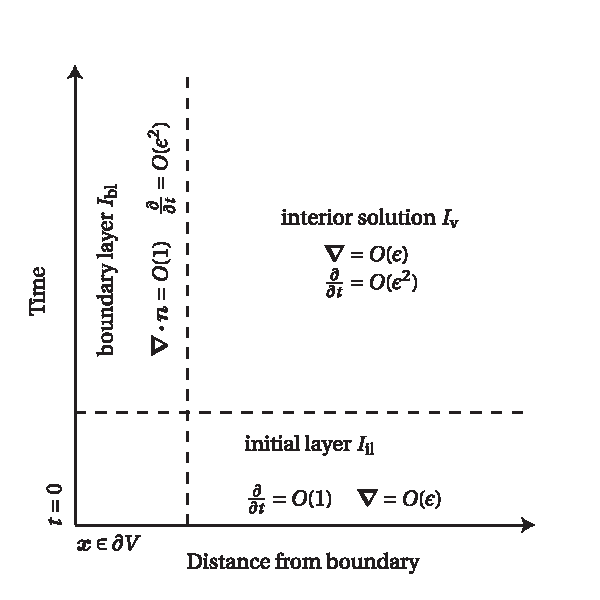
\includegraphics{layers}
  \caption{Depiction of interior, boundary layer, and initial layer of a
  transport problem.}
  \label{fig:layers}
\end{figure}

Our goal is first to develop an approximation to $\Iv$ that satisfies the transport
equation in some asymptotic limit, and then to use the boundary and initial layer
equations to ``match'' the interior solution to the transport solution on the
boundary and at the initial time. This procedure follows prior work in the
field, e.g.~the asymptotic derivation of the diffusion equation with
transport-matched boundary conditions \cite{Mal1991}.

%%%%%%%%%%%%%%%%%%%%%%%%%%%%%%%%%%%%%%%%%%%%%%%%%%%%%%%%%%%%%%%%%%%%%%%%%%%%%%%%
\subsection{Interior solution}\label{sec:adInterior}

The transport equation for the interior accounts for the extraneous source term,
but
it has no initial or boundary conditions, as it is only valid away from the
boundary and initial layer:
\begin{equation} \label{eq:tdVol}
  \frac{1}{c}\pder{\Iv}{t}(\vec{x},\vec{\Omega},t)
  + \vec{\Omega}\vd \grad \Iv(\vec{x},\vec{\Omega},t)
  + \sigma(\vec{x}) \Iv(\vec{x},\vec{\Omega},t)
  = \frac{\sigma_s(\vec{x})}{4\pi}
  \phi(\vec{x},t) + \frac{q(\vec{x},t)}{4\pi} \,.
\end{equation}
Here, we have defined
\begin{equation} \label{eq:tdPhi}
  \phi(\vec{x}) \equiv \int_{4\pi} \Iv(\vec{x}, \vec{\Omega},t) \ud \Omega\,,
\end{equation}
which is the \emph{interior} scalar intensity. We write Eq.~\eqref{eq:tdVol} as
\begin{equation*}
  \left[ \frac{1}{c}\pder{}{t}
  + \vec{\Omega}\vd \grad
  + \sigma \right] \Iv
  = \frac{\sigma_s}{4\pi}
  \phi + \frac{q}{4\pi} \,.
\end{equation*}

Taking the zeroth angular moment of Eq.~\eqref{eq:tdVol} gives a conservation
equation in the interior,
\begin{equation} \label{eq:loVol}
\frac{1}{c} \pder{\phi}{t} (\vec{x}, t)
  + \grad \vd\vec{F}(\vec{x}, t)
  + \sigma(\vec{x}) \phi(\vec{x}, t)
 = \sigma_s(\vec{x}) \phi(\vec{x},t) + q(\vec{x},t)\,.
\end{equation}
Here we have defined the interior radiation flux:
\begin{equation}\label{eq:tdF}
  \vec{F} \equiv \int_{4\pi} \vec{\Omega} \Iv(\vec{x}, \vec{\Omega},t) \ud
  \Omega\,,
\end{equation}
the first angular moment of the \emph{interior} solution.

Adding $\vec{\Omega}\vd \grad \phi$ to both sides of Eq.~\eqref{eq:loVol} and
multiplying the resulting equation by $\frac{1}{4\pi}$, we obtain
\begin{align*}
  \left[ \frac{1}{c}\pder{}{t}
  + \vec{\Omega}\vd \grad
  + \sigma \right]
  \left( \frac{1}{4\pi} \phi \right)
  = \frac{\sigma_s}{4\pi}
  \phi + \frac{q}{4\pi} - \frac{1}{4\pi} \grad \vd\vec{F} 
  + \frac{1}{4\pi} \vec{\Omega}\vd \grad \phi\,.
\end{align*}
Subtracting this equation from Eq.~\eqref{eq:tdVol} cancels the isotropic source
and scattering term on the right-hand side, yielding the following equation:
\begin{equation}\label{eq:capPsiVol}
  \left[ \frac{1}{c}\pder{}{t}
  + \vec{\Omega}\vd \grad
  + \sigma \right]
   \left( \Iv
  - \frac{1}{4\pi} \phi \right)
  = \frac{1}{4\pi} \grad \vd\vec{F} -
  \frac{1}{4\pi} \vec{\Omega}\vd \grad \phi\,.
\end{equation}

At this point, we apply an asymptotic scaling typical of a diffusive regime.
We make an ansatz that the spatial gradient of the solution is weak, the time
derivative is very small, and the solution is mildly (but not necessarily
linearly) anisotropic:
\begin{align} \label{eq:ansatz}
  \sigma &= O(1), &
  I &= O(1), &
  \int_{4\pi} \vec{\Omega} I \ud\Omega &= O(\epsilon), &
  \grad I &= O(\epsilon), &
  \pder{I}{t} &= O(\epsilon^2) \,.
\end{align}
These scalings are the same as in an asymptotic derivation of the standard
diffusion equation \cite{Lar1975,Mor2000}. With the scalings applied,
Eq.~\eqref{eq:capPsiVol} is written with the asymptotically small terms lumped
together:
\begin{equation*}
  \left[\vec{\Omega}\vd \grad
  + \sigma + O(\epsilon^2) \right]
   \left( \Iv
  - \frac{1}{4\pi} \phi \right)
  = - \frac{1}{4\pi} \vec{\Omega}\vd \grad \phi + O(\epsilon^2)\,.
\end{equation*}
Neglecting the high-order $O(\epsilon^2)$ terms, we make the first approximation
yet, obtaining:
\begin{equation}\label{eq:tdVolApprox1}
  \left[\vec{\Omega}\vd \grad  + \sigma \right]
   \left( \Iv
  - \frac{1}{4\pi} \phi \right)
  = - \frac{1}{4\pi} \vec{\Omega}\vd \grad \phi \,.
\end{equation}
Formally inverting the bracketed operator on the left-hand side, we obtain an
approximate expression for the intensity in the interior:
\begin{equation}\label{eq:tdVolApprox2}
  \Iv = \frac{1}{4\pi} \phi - 
  \left[\vec{\Omega}\vd \grad  + \sigma \right]\inv
  \left( \frac{1}{4\pi} \vec{\Omega}\vd \grad \phi \right)\,.
\end{equation}

The inverted differential operator is an integral transport operator
\cite{Pri2010}:
\begin{subequations} \label{eqs:inverseTransport}
  \begin{align} \label{eq:inverseTransportFull}
  \begin{split}
    \left[\vec{\Omega}\vd \grad  + \sigma \right]\inv
    \hat Q(\vec{x}, \vec{\Omega},t)
    &=
     \int_{0}^{\infty}
    \hat Q(\vec{x} - s \vec{\Omega}, \vec{\Omega}, t)
    \eexp^{ -\tau(\vec{x}, \vec{x} - s \vec{\Omega})}
    \ud s
\,.
  \end{split}
  \end{align}
  Here we have used the optical distance between points $\vec{x}$ and
  $\vec{x}'$ along the direction $\vec{\Omega} = (\vec{x}'-
  \vec{x})/\norm{\vec{x}'-\vec{x}}$:
  \begin{equation} \label{eq:fullTauDefinition}
    \tau(\vec{x}, \vec{x}') = \int_{0}^{\norm{\vec{x} -
    \vec{x}'}} \sigma(\vec{x}-s\vec{\Omega}) \ud s \,.
  \end{equation}
\end{subequations}

Thus Eq.~\eqref{eq:tdVolApprox2} for the interior intensity is a function of the
nonlocal, unknown scalar intensity:
\begin{equation}\label{eq:tdVolApprox1a}
  \Iv(\vec{x},\vec{\Omega},t) = \frac{1}{4\pi} \phi(\vec{x},t) - 
     \int_{0}^{\infty}
    \frac{1}{4\pi} \vec{\Omega}\vd \grad \phi(\vec{x} - s \vec{\Omega}, \vec{\Omega}, t)
    \eexp^{ -\tau(\vec{x}, \vec{x} - s \vec{\Omega})}
    \ud s \,.
\end{equation}
To simplify, we use the assumption from Eq.~\eqref{eq:ansatz} that spatial
gradients are weak to expand $\phi$ in a Taylor series about the local
point:
\begin{equation} \label{eq:taylorPhi}
  \phi(\vec{x} - s \vec{\Omega}, t)
  = \phi(\vec{x},t) - s\vec{\Omega} \vd
  \grad\phi (\vec{x}, t) + O(\epsilon^2) = \phi(\vec{x},t) +
  O(\epsilon) \,.
\end{equation}
Applying the truncated Taylor expansion to the gradient in
Eq.~\eqref{eq:tdVolApprox1a}, we obtain
\begin{equation*}
  \grad \phi(\vec{x}-s\vec{\Omega},t)
  = \grad \phi(\vec{x},t) + O(\epsilon^2)\,.
\end{equation*}
Thus, Eq.~\eqref{eq:tdVolApprox1a} becomes
\begin{align*}\nonumber
  \Iv(\vec{x},\vec{\Omega},t) &\approx \frac{1}{4\pi} \phi(\vec{x},t) - 
     \int_{0}^{\infty}
    \frac{1}{4\pi} \vec{\Omega}\vd \grad \phi(\vec{x} - s \vec{\Omega}, t)
    \eexp^{ -\tau(\vec{x}, \vec{x} - s \vec{\Omega})}
    \ud s
\\
  &= \frac{1}{4\pi} \phi(\vec{x},t) - \int_{0}^{\infty}
    \left[ \frac1{4\pi}\vec{\Omega}\vd \grad \phi(\vec{x},t) + O(\epsilon^2) \right]
    \eexp^{ -\tau(\vec{x}, \vec{x} - s \vec{\Omega})}
    \ud s
  \\ \nonumber
  &= \frac{1}{4\pi} \phi (\vec{x},t) - \left( \int_{0}^{\infty}
    \left[ \frac1{4\pi}\right]
    \eexp^{ -\tau(\vec{x}, \vec{x} - s \vec{\Omega})} \ud s \right)
    \vec{\Omega}\vd \grad \phi(\vec{x},t)
  \\
  &= \frac{1}{4\pi} \phi - 
  \left[\left(\vec{\Omega}\vd \grad  + \sigma \right)\inv
   \frac{1}{4\pi}\right] \left( \vec{\Omega}\vd \grad \phi \right) \,.
\end{align*}

We write this equation as
\begin{equation}\label{eq:tdVolApproxFinal}
  \Iv(\vec{x},\vec{\Omega},t)
  = \frac{1}{4\pi} \phi (\vec{x},t)
  - \left[ f(\vec{x}, \vec{\Omega}) \right] \vec{\Omega}\vd \grad \phi(\vec{x},t)\,,
\end{equation}
where we have defined
\begin{equation*}
  f(\vec{x},\vec{\Omega}) = \left(\vec{\Omega}\vd \grad  + \sigma \right)\inv
  \frac{1}{4\pi} \,,
\end{equation*}
which is the solution to the following differential transport equation:
\begin{equation} \label{eq:fVol}
  \vec{\Omega}\vd \grad f(\vec{x}, \vec{\Omega})
  + \sigma(\vec{x}) f (\vec{x}, \vec{\Omega})
= \frac{1}{4\pi} \,.
\end{equation}

Taking the first angular moment of Eq.~\eqref{eq:tdVolApproxFinal} gives the
approximate radiation flux in the interior:
\begin{align} \nonumber
  \vec{F}(\vec{x},t) &= \int_{4\pi} \vec{\Omega} \Iv(\vec{x},\vec{\Omega},t)
  \ud\Omega
  \\ \nonumber
  &= - \left[ \int_{4\pi} \vec{\Omega} \vec{\Omega} f(\vec{x}, \vec{\Omega}) \ud\Omega
  \right] \vd \grad \phi(\vec{x},t)
  \\ \label{eq:anisotropicFicks}
  &= - \Dtens(\vec{x}) \vd \grad \phi(\vec{x},t) \,.
\end{align}
This resembles ``Fick's law,'' but instead of a scalar diffusion
\emph{coefficient},
the anisotropic diffusion method has a diffusion \emph{tensor}, $\Dtens$, the
second angular moment of $f$:
\begin{equation}\label{eq:dDefinition}
  \Dtens(\vec{x}) \equiv \int_{4\pi} \vec{\Omega} \vec{\Omega}
  f(\vec{x}, \vec{\Omega}) \ud\Omega \,.
\end{equation}
In a homogeneous medium, $f\to\frac{1}{4\pi\sigma}$ and
$\Dtens\to\frac{1}{3\sigma}\Identitytens$: this reproduces Fick's law.

Because of the approximations made in developing Eq.~\eqref{eq:tdVolApproxFinal},
$\phi$ no longer satisfies the exact transport solution. Instead, like Fick's
law, the first-order accurate approximation to the radiation flux is substituted
into the low-order conservation equation~\eqref{eq:loVol} to yield an
anisotropic diffusion equation that $\phi$ satisfies in the interior:
\begin{equation} \label{eq:tdVolDiffusion}
\frac{1}{c} \pder{\phi}{t} (\vec{x}, t)
  - \grad \vd \Dtens(\vec{x}) \vd \grad \phi(\vec{x},t)
  + \sigma_a(\vec{x}) \phi(\vec{x}, t)
 = q(\vec{x},t)\,.
\end{equation}
Here we use the absorption opacity $\sigma_a = \sigma - \sigma_s$.

The anisotropic diffusion approximation to the interior solution $\Iv$
comprises \textsl{(i)} the transport equation~\eqref{eq:fVol} for $f$,
\textsl{(ii)} the definition in Eq.~\eqref{eq:dDefinition} of the diffusion
tensor $\Dtens$, and \textsl{(iii)} the anisotropic diffusion
equation~\eqref{eq:tdVolDiffusion}. We note that the transport equation for $f$
is very simple---it has no scattering. Thus, it is much less costly to solve
than the original transport problem.

%%%%%%%%%%%%%%%%%%%%%%%%%%%%%%%%%%%%%%%%%%%%%%%%%%%%%%%%%%%%%%%%%%%%%%%%%%%%%%%%
\clearpage
\subsection{Initial layer solution}

\newcommand{\phiil}{\phi_\mathrm{il}}
\newcommand{\Fil}{\vec{F}_\mathrm{il}}

The initial layer is a transport problem that accounts for the transition
between the initial condition and the interior solution, using
Eq.~\eqref{eq:tdSuperposition}. It is significant near the initial time $t=0$,
where the time derivatives are not assumed to be $O(\epsilon^2)$ but rather
$O(1)$. The problem is defined in the spatial interior of the problem, where
spatial gradients are $O(\epsilon)$, and the boundary layer
solution has decayed to zero. (See Fig.~\ref{fig:layers} for a depiction of the
initial layer in relation to the boundary layer and interior solution.)
We shall use the diffusion scaling that the absorption is very small: $\sigma_a
= \sigma - \sigma_s = O(\epsilon^2)$.

The transport problem for the initial layer
complements the interior transport equation~\eqref{eq:tdVol}, so it has no
extraneous source term:
\begin{subequations} \label{eqs:tdInit}
\begin{equation} \label{eq:ilVol}
  \frac{1}{c}\pder{\Iil}{t}(\vec{x},\vec{\Omega},t)
  + \epsilon \vec{\Omega}\vd \grad \Iil(\vec{x},\vec{\Omega},t)
  + \sigma(\vec{x}) \Iil(\vec{x},\vec{\Omega},t)
  = \frac{\sigma(\vec{x}) - \epsilon^2 \sigma_a(\vec{x})}{4\pi}
 \phiil(\vec{x},t) \,.
\end{equation}
Here we have defined the zeroth angular moment of the initial layer solution to
be
\begin{equation*}
  \phiil(\vec{x},t) \equiv \int_{4\pi} \Iil(\vec{x},\vec{\Omega},t) \ud
  \Omega \,.
\end{equation*}
The initial layer accounts for the original transport initial
condition in Eq.~\eqref{eq:tdTransportInit} via the superposition
equation~\eqref{eq:tdSuperposition}:
\begin{equation}\label{eq:ilInit}
 \Iv(\vec{x},\vec{\Omega},0) + \Iil(\vec{x},\vec{\Omega},0)
 = I^i(\vec{x},\vec{\Omega})\,.
\end{equation}
(The $\Ibl$ term is not present because, in the spatial interior, the boundary layer
solution has decayed away.)
Furthermore, by construction we demand that its solution rapidly tend to zero
for increasing $t$:
\begin{equation} \label{eq:ilLimit}
  \lim_{t\to\infty} \Iil(\vec{x},\vec{\Omega},t) = 0\,.
\end{equation}
\end{subequations}
The technique of asymptotic matching, which has previously applied to diffusion
in \cite{Mal1991,Lar1977}, uses this special transport problem to determine what
value the approximate interior solution $\phi$ should take at $t=0$ in order to
correctly match the transport solution.

The asymptotic analysis begins by expanding $\Iil$ in powers of $\epsilon$,
\begin{equation*}
  \Iil(\vec{x},\vec{\Omega},t) \sim \Iil^{(0)}(\vec{x},\vec{\Omega},t)
  + \epsilon \Iil^{(1)}(\vec{x},\vec{\Omega},t)
  + \epsilon^2 \Iil^{(2)}(\vec{x},\vec{\Omega},t)
  + \cdots\,,
\end{equation*}
and substituting into the scaled transport equation~\eqref{eq:ilVol}. The zeroth
moment of the
initial layer solution is also written as a series expansion:
\begin{equation*}
  \phiil(\vec{x},t) \sim \phiil^{(0)}(\vec{x},t)
  + \epsilon \phiil^{(1)}(\vec{x},t)
  + \epsilon^2 \phiil^{(2)}(\vec{x},t)
  + \cdots\,.
\end{equation*}
Finally, we write the interior solution $\Iv$ by expanding the interior solution
in powers of $\epsilon$:
\begin{equation*}
  \phi(\vec{x},t) \sim \phi^{(0)}(\vec{x},t)
  + \epsilon \phi^{(1)}(\vec{x},t)
  + \cdots\,.
\end{equation*}
Replacing $\vec{\Omega}\vd\grad$ with $\epsilon \vec{\Omega}\vd\grad$, the
anisotropic diffusion approximation in the interior,
Eq.~\eqref{eq:tdVolApproxFinal}, is:
\begin{align*}
  \Iv
 &= \frac{1}{4\pi} \left( \phi^{(0)} + \epsilon \phi^{(1)} + \cdots\right)
  - \epsilon f \vec{\Omega} \vd \grad \left( \phi^{(0)}
    + \epsilon \phi^{(1)} + \cdots\right)
\\
  &= \frac{1}{4\pi} \phi^{(0)} + \epsilon \left[ \frac{1}{4\pi} \phi^{(1)}
    - f \vec{\Omega} \vd \grad \phi^{(0)} \right] + O(\epsilon^2)\,.
\end{align*}
Thus the initial condition for the initial layer, Eq.~\eqref{eq:ilInit},
becomes
\begin{equation}\label{eq:ilInit2}
 \frac{1}{4\pi} \phi^{(0)}(0) + \epsilon \left[ \frac{1}{4\pi} \phi^{(1)}(0)
    - f \vec{\Omega} \vd \grad \phi^{(0)}(0) \right] 
    + \Iil^{(0)}(0) + \epsilon  \Iil^{(1)}(0) + O(\epsilon^2)
 = I^i(\vec{x},\vec{\Omega})\,.
\end{equation}

For Eq.~\eqref{eq:ilInit2} to hold, the components of each power of
$\epsilon$ must match. Additionally, to satisfy Eq.~\eqref{eq:ilLimit}, each
expanded term of the initial layer solution must also rapidly
tend to zero. We begin by matching the $O(1)$ terms in the initial layer
equation~\eqref{eq:ilVol}:
\begin{equation}\label{eq:ilVolZeroth}
  \frac{1}{c}\pder{\Iil^{(0)}}{t}
  + \sigma \Iil^{(0)}
  = \frac{\sigma}{4\pi} \phiil^{(0)} \,.
\end{equation}
Taking the zeroth moment of this equation, we find that the number of particles
in the leading term of the initial layer is constant:
\begin{equation}\label{eq:ilVolZeroth2}
  \frac{1}{c}\pder{\phiil^{(0)}}{t} = 0 \,.
\end{equation}
Thus to satisfy Eq.~\eqref{eq:ilLimit}, $\phiil^{(0)}$ must be zero at the initial
time:
\begin{equation*}
  \phiil^{(0)}(0) = 0\,.
\end{equation*}
To use this fact, we take the leading order terms of the initial condition,
Eq.~\eqref{eq:ilInit2}:
\begin{equation*}
 \frac{1}{4\pi} \phi^{(0)}(0) + \Iil^{(0)}(0) = I^i(\vec{x},\vec{\Omega})\,,
\end{equation*}
and integrate over all angles to obtain
\begin{equation}\label{eq:ilInitZeroth}
 \phi^{(0)}(0) + \phiil^{(0)}(0) = \phi^i\,.
\end{equation}
Here we have defined the zeroth moment of the initial condition
\begin{equation*}
  \phi^i(\vec{x}) = \int_{4\pi} I^i(\vec{x},\vec{\Omega}) \ud\Omega\,.
\end{equation*}
Setting $\phiil^{(0)}(0) = 0$, we obtain a relation between the leading order scalar
intensity in the interior and the zeroth moment of the transport initial
condition:
\begin{equation}\label{eq:ilZeroth}
  \phi^{(0)}(\vec{x}, 0) = \phi^i(\vec{x})\,.
\end{equation}
This is the condition for $\phi$ at the initial time to eliminate the leading
order component of the initial layer in the temporal interior of the problem:
\begin{equation*}
  \phi(\vec{x},0) = \phi^i(\vec{x}) + O(\epsilon)\,.
\end{equation*}
Because the anisotropic diffusion solution is $O(\epsilon^2)$-accurate in the
interior of a diffusive problem, we desire an initial condition that has an
additional order of accuracy.

The first step in solving for the $O(\epsilon^2)$-accurate initial condition is
to exactly solve for the $O(1)$ component of $\Iil$ in
Eq.~\eqref{eq:ilVolZeroth} for all times, using the fact that $\phiil^{(0)}=0$:
\begin{equation*}
  \frac{1}{c}\pder{\Iil^{(0)}}{t} + \sigma \Iil^{(0)} = 0
  \lra \Iil^{(0)}(t) = \Iil^{(0)}(0) \eexp^{-\sigma c t} \,.
\end{equation*}
We solve for $\Iil^{(0)}(0)$ in Eq.~\eqref{eq:ilVolZeroth2} to find
\begin{equation*}
 \Iil^{(0)}(t) \left[ I^i - \frac{\phi^i}{4\pi} \right] \eexp^{-\sigma c t}\,.
\end{equation*}
Now we turn to the $O(\epsilon)$ component of the initial layer equation:
\begin{equation*}
  \frac{1}{c}\pder{\Iil^{(1)}}{t}
  + \vec{\Omega}\vd \grad \Iil^{(0)}
  + \sigma \Iil^{(1)}
  = \frac{\sigma}{4\pi} \phiil^{(1)} \,.
\end{equation*}
Substituting the solution $\Iil^{(0)}$, we obtain
\begin{equation}\label{eq:ilVolFirst}
  \frac{1}{c}\pder{\Iil^{(1)}}{t}
  + \sigma \Iil^{(1)}
  = \frac{\sigma}{4\pi} \phiil^{(1)}
  -  \vec{\Omega}\vd \grad \left[\left(  I^i - \frac{\phi^i}{4\pi} \right)
    \eexp^{-\sigma c t} \right] \,.
\end{equation}
Integrating Eq.~\eqref{eq:ilVolFirst} over angle eliminates the absorption
term, since the problem is assumed to be purely scattering to $O(\epsilon)$,
and yields:
\begin{equation*}
  \frac{1}{c}\pder{\phiil^{(1)}}{t}
  = - \grad \vd \left[\vec{F}^i \eexp^{-\sigma c t} \right] \,,
\end{equation*}
where the initial radiation flux is
\begin{equation*}
  \vec{F}^i = \int_{4\pi} \vec{\Omega} I^i(\vec{x},\vec{\Omega})\ud\Omega\,.
\end{equation*}

We solve the differential equation for $\phiil^{(1)}(t)$:
\begin{equation*}
  \phiil^{(1)}(t) = \phiil^{(1)}(0) - \grad \vd \left[\frac{\vec{F}^i}{\sigma}
    \left( 1 - \eexp^{-\sigma c t} \right) \right] \,.
\end{equation*}
Taking the limit as $t\to\infty$ and demanding that it satisfy
Eq.~\eqref{eq:ilLimit}, we obtain a relation that the first-order initial
layer must satisfy:
\begin{equation}\label{eq:ilVolFirst2}
  0 = \phiil^{(1)}(0) - \grad \vd \left[\frac{\vec{F}^i}{\sigma} \right] \,.
\end{equation}

The first-order terms of the initial condition, Eq.~\eqref{eq:ilInit2}, are:
\begin{equation*}
 \frac{1}{4\pi} \phi^{(1)}(0)
 + f \vec{\Omega} \vd \grad \phi^{(0)}(0)
 + \Iil^{(1)}(0) = 0\,.
\end{equation*}
The zeroth angular moment of this equation is:
\begin{equation}\label{eq:ilInitFirst}
 \phi^{(1)}(0)
 + \int_{4\pi}\vec{\Omega} f \ud\Omega \vd \grad \phi^{(0)}(0)
 + \phiil^{(1)}(0) = 0\,.
\end{equation}
We apply the known $\phi^{(0)}(0)$ from
Eq.~\eqref{eq:ilZeroth}, and the condition on the first-order initial layer
from Eq.~\eqref{eq:ilVolFirst2}:
\begin{equation}\label{eq:ilFirst}
 \phi^{(1)}(0) = 
 - \int_{4\pi}\vec{\Omega} f \ud\Omega \vd \grad \phi^i
 - \grad \vd \left(\frac{\vec{F}^i}{\sigma} \right)\,.
\end{equation}
Combining Eqs.~\eqref{eq:ilZeroth} and~\eqref{eq:ilFirst} give the
transport-matched initial condition for the interior to first order accuracy
in $\epsilon$:
\begin{equation}\label{eq:ilMatched}
  \phi(\vec{x},0) = \phi^i(\vec{x})
- \epsilon \left[ \int_{4\pi}\vec{\Omega} f \ud\Omega \vd \grad \phi^i(\vec{x})
+ \grad \vd \left(\frac{\vec{F}^i(\vec{x})}{\sigma(\vec{x})} \right) \right]
\,.
\end{equation}
In a homogeneous medium, $f$ is isotropic and the second term is zero. The
remainder is the standard diffusion result \cite{Mal1991},
\begin{equation*}
 \phi(0) = \phi^i - \epsilon\grad \vd \left[\frac{\vec{F}^i}{\sigma} \right]\,.
\end{equation*}

To summarize: the initial condition on $\phi$ that preserves the leading-order
component of the transport solution is:
\begin{equation*}
  \phi(\vec{x},0) = \phi^i(\vec{x}) \equiv 
  \phi^i(\vec{x}) = \int_{4\pi} I^i(\vec{x},\vec{\Omega}) \ud\Omega\,.
\end{equation*}
To match the transport solution and interior solution to \emph{first} order
accuracy in $\epsilon$, the potentially nonconservative
Eq.~\eqref{eq:ilMatched} should be used. However, in the rest of this work, we
shall only use the leading-order accurate equation for the following reasons:
\begin{itemize}
  \item In a truly diffusive problem where this initial layer analysis is
    applicable, $f$ is isotropic to leading order, so the second term of
    Eq.~\eqref{eq:ilMatched} may be discarded while retaining $O(\epsilon^2)$
    accuracy.
  \item When the initial condition is isotropic, $\vec{F}^i=0$, and the third
    term in Eq.~\eqref{eq:ilMatched} is identically zero.
  \item Using the nonconservative form in a radiation transport problem may
    violate the conservation of energy.
  \item The nonconservative $O(\epsilon)$-accurate form is not commonly used in
    practice.
\end{itemize}

%%%%%%%%%%%%%%%%%%%%%%%%%%%%%%%%%%%%%%%%%%%%%%%%%%%%%%%%%%%%%%%%%%%%%%%%%%%%%%%%
\subsection{Boundary layer solution}\label{sec:adBoundary}

Near the exterior problem boundary, away from the initial time, the transport
solution rapidly transitions to the interior solution in the \emph{boundary
layer}. (Figure~\ref{fig:layers} graphically depicts the relationship of
the boundary layer to the interior solution.)
The
spatial gradient normal to the boundary is $O(1)$, and the time
derivative is $O(\epsilon^2)$. The transport equation for the boundary layer is
source-free:
\begin{subequations} \label{eqs:tdBndy}
  \begin{equation} \label{eq:tdBndyVol}
    \frac{1}{c}\pder{}{t} \Ibl(\vec{x},\vec{\Omega},t)
  + \vec{\Omega}\vd \grad \Ibl(\vec{x},\vec{\Omega},t)
  + \sigma(\vec{x}) \Ibl(\vec{x},\vec{\Omega},t)
  = \frac{\sigma_s(\vec{x})}{4\pi}
  \int_{4\pi} \Ibl(\vec{x},\vec{\Omega}',t) \ud \Omega' \,.
\end{equation}
This equation accounts for the transport boundary condition,
Eq.~\eqref{eq:tdTransportBndy}, using the superposition relation of
Eq.~\eqref{eq:tdSuperposition}:
\begin{equation} \label{eq:tdBndyBndy}
\Iv(\vec{x},\vec{\Omega},t)
+ \Ibl(\vec{x},\vec{\Omega},t)
 = I^b(\vec{x},\vec{\Omega},t) \,,
  \quad \vec{x}\in \partial V ,\ \vec{\Omega}\vd \vec{n} < 0,
\end{equation}
(Here we have used $\Iil=0$ because the initial layer solution has decayed
away, as the boundary layer is defined away from $t=0$.)
We demand that the boundary layer solution rapidly tend to zero with increasing
distance $s$ from the boundary along the direction $-\vec{\Omega}$:
\begin{equation} \label{eq:tdBndyLimit}
  \lim_{s \to\infty} \Ibl(\vec{x},\vec{\Omega},t)
  = 0 \,.
\end{equation}
\end{subequations}

If the boundary condition $I^b$ varies slowly in space, and the radius of
curvature of
the exterior is large, then it can be shown \cite{Mal1991} that the condition
that satisfies Eqs.~\eqref{eqs:tdBndy} to leading order is:
\begin{equation}\label{eq:tdKillBndy}
  \int_{\vec{\Omega}\vd\vec{n} < 0}
  W(\abs{\vec{\Omega}\vd\vec{n}}) \Ibl(\vec{x},\vec{\Omega},t) \ud\Omega
  = 0\,,
  \quad \vec{x}\in \partial V ,\ \vec{\Omega}\vd \vec{n} < 0.
\end{equation}
Here, $W$ is related to Chandrasekhar's $H$-function \cite{Cha1960}:
\begin{equation} \label{eq:chandraW}
  W(\mu) = \frac{\sqrt{3}}{2} \mu H(\mu)
  \approx \mu + \tfrac{3}{2} \mu^2 \,, \quad 0 < \mu \le 1 .
\end{equation}
The polynomial approximation is derived variationally \cite{Mal1991} and is
accurate to
second order when used inside the integral in Eq.~\eqref{eq:tdKillBndy}.
The Marshak boundary condition uses $W(\mu) \approx 2 \mu$.

Multiplying Eq.~\eqref{eq:tdBndyBndy} by $W(\mu)$, integrating over incident
directions on the exterior boundary, and substituting
Eq.~\eqref{eq:tdKillBndy} to demand that the boundary layer vanish in the
interior, we obtain
the following relation:
\begin{equation*}
  \int_{\vec{\Omega}\vd\vec{n} < 0}
  W(\abs{\vec{\Omega}\vd\vec{n}})
\Iv(\vec{x},\vec{\Omega},t) \ud\Omega
+ 0
= 
  \int_{\vec{\Omega}\vd\vec{n} < 0}
  W(\abs{\vec{\Omega}\vd\vec{n}})
I^b(\vec{x},\vec{\Omega},t) \ud\Omega \,.
\end{equation*}
Substituting the interior approximation of Eq.~\eqref{eq:tdVolApproxFinal}, we find:
\begin{align*} \nonumber
\lefteqn{\int_{\vec{\Omega}\vd\vec{n} < 0} W(\abs{\vec{\Omega}\vd\vec{n}})
I^b(\vec{x},\vec{\Omega},t) \ud\Omega}
\qquad&
\\ \nonumber
&= 
\int_{\vec{\Omega}\vd\vec{n} < 0}
W(\abs{\vec{\Omega}\vd\vec{n}})
\left[  \frac{1}{4\pi} \phi (\vec{x},t)
  - f(\vec{x}, \vec{\Omega})\vec{\Omega}\vd \grad \phi(\vec{x},t)
\right] \ud \Omega
\\ \nonumber
&=
\frac{1}{4\pi} \phi(\vec{x},t)
\int_{\vec{\Omega}\vd\vec{n} < 0} W(\abs{\vec{\Omega}\vd\vec{n}}) \ud\Omega
- \left[ \int_{\vec{\Omega}\vd\vec{n} < 0}  W(\abs{\vec{\Omega}\vd\vec{n}})
f(\vec{x}, \vec{\Omega})\vec{\Omega} \ud\Omega\right] \vd \grad \phi(\vec{x},t)
\\
&= \frac{1}{2} \phi(\vec{x},t)
- \left[ \int_{\vec{\Omega}\vd\vec{n} < 0} W(\abs{\vec{\Omega}\vd\vec{n}})
\vec{\Omega} f(\vec{x}, \vec{\Omega}) \ud\Omega\right] \vd \grad \phi(\vec{x},t)\,.
\end{align*}
Multiplying by two, we arrive at the low-order boundary condition for the
anisotropic diffusion approximation:
\begin{equation*}
2\int_{\vec{\Omega}\vd\vec{n} < 0} W(\abs{\vec{\Omega}\vd\vec{n}})
I^b(\vec{x},\vec{\Omega},t) \ud\Omega
=
\phi(\vec{x},t)
+ 2 \left[ -\int_{\vec{\Omega}\vd\vec{n} < 0} W(\abs{\vec{\Omega}\vd\vec{n}})
\vec{\Omega} f(\vec{x}, \vec{\Omega}) \ud\Omega\right] \vd \grad \phi(\vec{x},t)\,.
\end{equation*}
To make this equation clearer, we define the bracketed vector term to be
\begin{equation}\label{eq:adBoundaryIntegral}
  \vec{d}(\vec{x}) = -\int_{\vec{\Omega}\vd\vec{n} < 0} W(\abs{\vec{\Omega}\vd\vec{n}})
\vec{\Omega} f(\vec{x}, \vec{\Omega}) \ud\Omega\,,
\end{equation}
so that the boundary condition on $\phi$ becomes
\begin{equation} \label{eq:loBc}
2\int_{\vec{\Omega}\vd\vec{n} < 0} W(\abs{\vec{\Omega}\vd\vec{n}})
I^b(\vec{x},\vec{\Omega},t) \ud\Omega
=
\phi(\vec{x},t)
+ 2 \vec{d}(\vec{x}) \vd \grad \phi(\vec{x},t)\,.
\end{equation}
Here, $\vec{d}$ is a vector defined on the boundary, $\vec{x} \in \partial V$,
that is calculated from the incident values of the purely absorbing
transport solution $f$.

The boundary condition is at this point incomplete, because the
transport
solution for $f$ has only been defined for points away from the boundary: the
prescription of $f$ for incident directions on the boundary is unknown.
We return to
the definition of $\phi$ in Eq.~\eqref{eq:tdPhi} and substitute the approximated
interior intensity from Eq.~\eqref{eq:tdVolApproxFinal}:
\begin{align*}
  \phi(\vec{x},t) &= \int_{4\pi} \left[ 
\frac{1}{4\pi} \phi (\vec{x},t)
  - f(\vec{x}, \vec{\Omega})\vec{\Omega}\vd \grad \phi(\vec{x},t)
  \right] \ud \Omega
  \\
  \phi(\vec{x},t) &= \phi (\vec{x},t)
  - \int_{4\pi} f(\vec{x}, \vec{\Omega})\vec{\Omega} \ud \Omega
  \vd \grad \phi(\vec{x},t)
  \\
  0 &= - \left[ \int_{4\pi} f(\vec{x}, \vec{\Omega})\vec{\Omega} \ud\Omega
  \right]
  \vd \grad \phi(\vec{x},t) \,.
\end{align*}
\emph{The above equation is not generally satisfied}. It does hold true when
$f$ is an ``even'' function of $\vec{\Omega}$, e.g.\ in an optically thick,
homogeneous material, where $f$ is isotropic. At material
boundaries, $f$ can be strongly anisotropic, and the above relation is not
satisfied. By requiring $\int_{4\pi} \Iv \ud\Omega = \phi$ at exterior
boundaries, we
obtain a relationship between the ``known'' outgoing values of $f$ and the
unknown incoming:
\begin{equation*}
  0 =
  \int_{\vec{\Omega}\vd\vec{n} > 0} \vec{\Omega} f(\vec{x}, \vec{\Omega}) \ud \Omega
 + \int_{\vec{\Omega}\vd\vec{n} < 0} \vec{\Omega} f(\vec{x}, \vec{\Omega}) \ud
 \Omega\,.
\end{equation*}
If the opacity varies slowly along the boundary (which is a precondition for the
analogous standard diffusion boundary condition), then to leading order, $f$
is azimuthally symmetric about the outward normal at the boundary. The above
relation is then equivalent to the following:
\begin{equation}\label{eq:hoBc}
  \int_{\vec{\Omega}\vd\vec{n} > 0} (\vec{\Omega}\vd \vec{n})
  f(\vec{x}, \vec{\Omega}) \ud\Omega
  =
  \int_{\vec{\Omega}\vd\vec{n} < 0} \abs{\vec{\Omega}\vd \vec{n}}
  f(\vec{x}, \vec{\Omega}) \ud\Omega \,.
\end{equation}
Thus, the transport equation for $f$ should have boundary conditions
that enforce this relationship. Both specularly reflecting and
``white'' boundary conditions satisfy Eq.~\eqref{eq:hoBc}.
The above condition does not \emph{define} the boundary condition for $f$; it
is only a restriction that preserves Eq.~\eqref{eq:tdPhi}.

In the case when $f$ is azimuthally symmetric about the outward normal,
Eq.~\eqref{eq:adBoundaryIntegral} can be written:
\begin{equation*}
  \vec{d}(\vec{x}) = -\int_{\vec{\Omega}\vd\vec{n} < 0} W(\abs{\vec{\Omega}\vd\vec{n}})
  (-\abs{ \vec{\Omega} \vd \vec{n}} \vec{n})
  f(\vec{x}, \vec{\Omega}) \ud\Omega\,,
\end{equation*}
thereby simplifying to the following expression:
\begin{equation} \label{eq:adBoundaryIntegral2}
  \vec{d}(\vec{x})
  = \left[ \int_{\vec{\Omega}\vd\vec{n} < 0}
  \abs{\vec{\Omega}\vd\vec{n}} W(\abs{\vec{\Omega}\vd\vec{n}})
  f(\vec{x}, \vec{\Omega}) \ud\Omega\right] \vec{n}\,.
\end{equation}
Thus the vector quantity $\vec{d}$ lives on the boundary, points along the
outward normal, and has a positive magnitude that depends on the incident
distribution of $f$. If $f$ is isotropic and equal to the infinite medium value
$1/(4\pi\sigma)$, then $\norm{\vec{d}}$ reduces to $z_0 / (2 \sigma)$, where
$z_0$ is the transport-corrected extrapolation distance for diffusion,
and Eq.~\eqref{eq:loBc} becomes the transport-corrected standard diffusion
boundary condition with transport extrapolation distance.

%%%%%%%%%%%%%%%%%%%%%%%%%%%%%%%%%%%%%%%%
\subsubsection{Marshak-like boundary condition}

One distribution for the incident $f$ that satisfies
Eq.~\eqref{eq:hoBc} is a specularly reflecting boundary:
\begin{equation} \label{eq:zetaReflecting}
  f(\vec{x}, \vec{\Omega}) = f(\vec{x}, \vec{\Omega}_r) \,,
 \quad \vec{x} \in \partial V, \ \vec{\Omega} \vd \vec{n} < 0 \,.
\end{equation}
Here, $\vec{\Omega}_r$ is the reflected angle on a boundary surface with outward
normal $\vec{n}$:
\begin{equation} \label{eq:reflection}
  \vec{\Omega}_r = \vec{\Omega} - 2(\vec{\Omega} \vd \vec{n}) \vec{n}\,.
\end{equation}

The choice of a reflecting boundary has a particular advantage if we use the
``Marshak'' approximation
that $W(\mu)\approx 2\mu$. Equation~\eqref{eq:loBc} becomes
\begin{align*}
  2\int_{\vec{\Omega}\vd \vec{n} < 0}
  ( 2\abs{\vec{\Omega} \vd \vec{n}} ) I^b(\vec{\Omega}) \ud\Omega
  &= \phi
  + 2\vec{d} \vd \grad \phi
  \\
  4 F^-
  &= \phi
  + 2\vec{d} \vd \grad \phi
\end{align*}

With the Marshak approximation to $W(\mu)$, the expression for $\vec{d}$
simplifies greatly.  Equation~\eqref{eq:adBoundaryIntegral}, becomes
\begin{align*}
  \vec{d} &=
  -\int_{\vec{\Omega}\vd\vec{n} < 0} 2 \abs{\vec{\Omega}\vd\vec{n}}
  \vec{\Omega} f \ud\Omega
  \\
  &= 
  2 \vec{n}\vd \int_{\vec{\Omega}\vd\vec{n} < 0} \vec{\Omega}
  \vec{\Omega} f \ud\Omega
  \\
  \intertext{Because our chosen boundary condition of $f$ gives
  $f(\vec{\Omega})=f(-\vec{\Omega})$ if $f$ is azimuthally symmetric, the
  integrand is an even function of $\vec{\Omega}$:}
  \\
   \vec{d} &=
  \vec{n}\vd\int_{4\pi} \vec{\Omega} \vec{\Omega} f \ud\Omega \,.
  \\ 
  \intertext{The integral on the right hand side is the anisotropic diffusion
  tensor from Eq.~\eqref{eq:anisotropicFicks}:}
  \vec{d} &= \vec{n}\vd\Dtens \,.
\end{align*}

Thus Marshak-like boundary approximation for anisotropic diffusion is:
\begin{equation}\label{eq:marshakAd}
  4 F^-(\vec{x}, t)
  = \phi(\vec{x}, t)
  + 2 \vec{n} \vd \Dtens(\vec{x}) \vd \grad \phi(\vec{x}, t) \,.
\end{equation}
This is analogous to the standard diffusion Marshak boundary condition,
\begin{equation*}
  4 F^-(\vec{x}, t) = \phi(\vec{x}, t)
  + 2 D(\vec{x}) \vec{n} \vd \grad \phi(\vec{x}, t)\,.
\end{equation*}

%%%%%%%%%%%%%%%%%%%%%%%%%%%%%%%%%%%%%%%%
\subsection{Summary}
We have now derived a full description of the time-dependent anisotropic
diffusion equations in a finite medium. 

The anisotropic diffusion method approximates the transport
equations~\eqref{eqs:tdTransport} with a set of low-order equations for the
scalar intensity $\phi$ that use a diffusion tensor calculated from a
simple high-order transport equation.

The low order equation is the result of substituting the approximate Fick's law,
Eq.~\eqref{eq:anisotropicFicks}, into the conservation equation~\eqref{eq:loVol}:
\begin{equation*}
\frac{1}{c} \pder{\phi}{t} (\vec{x}, t)
  - \grad \vd \Dtens(\vec{x}) \vd \grad \phi(\vec{x},t)
  + \sigma(\vec{x}) \phi(\vec{x}, t)
  = Q(\vec{x}, t) \,,
  \quad \vec{x} \in V,\ t > 0 \,.
\end{equation*}
From the initial layer analysis, the initial condition is to leading order:
\begin{equation*}
  \phi(\vec{x}, 0) = \int_{4\pi} I^i(\vec{x},\vec{\Omega}) \ud\Omega \,,
  \quad \vec{x} \in V  \,.
\end{equation*}
The incident source boundary condition with the simpler Marshak-like
approximation from Eq.~\eqref{eq:marshakAd} is
\begin{equation*}
  4 F^-(\vec{x}, t)
  = \phi(\vec{x}, t)
  + 2 \vec{n} \vd \Dtens(\vec{x}) \vd \grad \phi(\vec{x}, t) \,,
 \quad \vec{x} \in \partial V,\ t > 0\,.
\end{equation*}

The anisotropic diffusion tensor is defined in Eq.~\eqref{eq:dDefinition},
\begin{equation*}
  \Dtens(\vec{x}) \equiv \int_{4\pi} \vec{\Omega} \vec{\Omega}
  f(\vec{x}, \vec{\Omega}) \ud\Omega \,,
\end{equation*}
where $f$ is the solution of the steady-state, purely absorbing transport
equation described by Eq.~\eqref{eq:fVol}:
\begin{subequations} \label{eqs:fFull}
\begin{equation}\label{eq:fFullVol}
  \vec{\Omega}\vd \grad f(\vec{x}, \vec{\Omega})
  + \sigma f (\vec{x}, \vec{\Omega})
  = \frac{1}{4\pi} \,, \quad x \in V,\ \vec{\Omega} \in 4\pi\,.
\end{equation}
In conjunction with the Marshak boundary condition, $f$ should be reflecting on
the problem boundary:
\begin{equation}\label{eq:fFullBndy}
  f(\vec{x}, \vec{\Omega}) = f(\vec{x}, \vec{\Omega}_r) \,,
 \quad \vec{x} \in \partial V, \ \vec{\Omega} \vd \vec{n} < 0 \,.
\end{equation}
\end{subequations}

In the more general case when Eq.~\eqref{eq:loBc} is used, $f$ only needs to
satisfy the relation given in Eq.~\eqref{eq:hoBc}:
\begin{equation*}
  \int_{\vec{\Omega}\vd\vec{n} > 0} (\vec{\Omega}\vd \vec{n})
  f(\vec{x}, \vec{\Omega}) \ud\Omega
  =
  \int_{\vec{\Omega}\vd\vec{n} < 0} \abs{\vec{\Omega}\vd \vec{n}}
  f(\vec{x}, \vec{\Omega}) \ud\Omega \,.
\end{equation*}
The corresponding transport-matched low-order boundary condition from
Eq.~\eqref{eq:loBc} is:
\begin{equation*}
2\int_{\vec{\Omega}\vd\vec{n} < 0} W(\abs{\vec{\Omega}\vd\vec{n}})
I^b(\vec{x},\vec{\Omega},t) \ud\Omega
=
\phi(\vec{x},t)
+ 2 \vec{d}(\vec{x}) \vd \grad \phi(\vec{x},t)\,,
\end{equation*}
where $\vec{d}$ is defined in Eq.~\eqref{eq:adBoundaryIntegral} as a function
of the incident values for $f$, written here under the assumption that $f$ is
rotationally invariant about the outward normal at the boundary:
\begin{equation*}
  \vec{d}(\vec{x})
  = \left[ \int_{\vec{\Omega}\vd\vec{n} < 0}
  \abs{\vec{\Omega}\vd\vec{n}} W(\abs{\vec{\Omega}\vd\vec{n}})
  f(\vec{x}, \vec{\Omega}) \ud\Omega\right] \vec{n}\,.
\end{equation*}

%%%%%%%%%%%%%%%%%%%%%%%%%%%%%%%%%%%%%%%%%%%%%%%%%%%%%%%%%%%%%%%%%%%%%%%%%%%%%%%%
\section{Discussion}
Even without numerical results for the anisotropic diffusion equations, a
number of interesting and beneficial properties can be deduced from the
low-order AD equations and the transport equations for $f$.

%%%%%%%%%%%%%%%%%%%%%%%%%%%%%%%%%%%%%%%%
\subsection{Application to nonlinear radiation transport}
\label{sec:appNonlinear}

In \S\ref{sec:adDerivation}, the asymptotic analysis was performed only for
linear time-dependent transport equation rather than to the nonlinear system of
TRT equations. (For a rigorous asymptotic analysis of the TRT equations, see
\cite{Lar1983a}.) To apply our results to TRT, we appeal to two facts.

First, the implementation of the TRT equations in this thesis uses the
semi-implicit linearization from \S\ref{sec:bgSemiImplicit}. In that form, the
TRT equations over a time step are reduced to a linear transport equation with
an isotropic scattering term. Thus the linear asymptotic analysis presented here
is applicable to that linearized radiation equation.

Second, if the standard diffusion scaling is taken, the anisotropic diffusion
equations yield the standard diffusion result to first order. To see this, we
apply the scaling $\vec{\Omega}\vd \grad \to \epsilon \vec{\Omega}\vd \grad$ to
the transport equation for $f$ in Eq.~\eqref{eq:fFullVol}:
\begin{equation*}
  \epsilon \vec{\Omega}\vd \grad f(\vec{x}, \vec{\Omega}, t)
  + \sigma(\vec{x},t) f(\vec{x}, \vec{\Omega}, t)
  = \frac{1}{4\pi}\,.
\end{equation*}
Here, we have assumed a time-dependent opacity and, resultantly, $f$ depends on
time as a parameter (not a variable). Solving for $f$ as a series expansion in
$\epsilon$, we find:
\begin{align*}
  f(\vec{x}, \vec{\Omega}, t)
  \sim
  \frac{1}{4\pi \sigma}
  - \epsilon 
  \frac{1}{\sigma} \vec{\Omega}\vd \grad \frac{1}{4\pi \sigma}
  + O( \epsilon^2)\,.
\end{align*}
Taking the second angular moment, we obtain a diffusion tensor isotropic to
first order:
\begin{equation*}
  \Dtens(\vec{x}, t)
  =
  \frac{1}{3 \sigma} \Identitytens
  - 0
  + O( \epsilon^2)\,.
\end{equation*}
Substituting this into the anisotropic Fick's law yields the standard Fick's
law:
\begin{equation*}
  \vec{F}(\vec{x},t) = - \frac{1}{3 \sigma(\vec{x},t)} \grad \phi(\vec{x},t)\,.
\end{equation*}
In other words, in the diffusion limit, anisotropic diffusion is equivalent to
diffusion, to first order.

We therefore assert that the anisotropic diffusion method will
satisfy the conventional diffusive limit of the transport equation for thermal
radiative transport.

The low-order anisotropic diffusion equation for TRT is
\begin{equation*}
\frac{1}{c} \pder{\phi}{t} (\vec{x}, t)
  - \grad \vd \Dtens(\vec{x},t) \vd \grad \phi(\vec{x},t)
  + \sigma(\vec{x}, T[\vec{x}, t]) \phi(\vec{x}, t)
  = \sigma(\vec{x}) ac [T(\vec{x}, t)]^4 + q_{r}(\vec{x}, t)\,,
\end{equation*}
where the anisotropic diffusion tensor depends on the temperature-dependent
opacity $\sigma$ via the transport equation for $f$:
\begin{equation*}
  \vec{\Omega}\vd \grad f(\vec{x}, \vec{\Omega}, t)
  + \sigma(\vec{x},T[\vec{x},t]) f(\vec{x}, \vec{\Omega}, t)
  = \frac{1}{4\pi}\,.
\end{equation*}
In this transport problem for $f$, the time $t$ is a parameter, not a variable:
the time dependence of $f$ is due entirely to the time-dependence of $\sigma$.
When the semi-implicit approximation is made that freezes $\sigma$ at the
beginning of the time step, there is no feedback between $\phi$ and $f$ during a
time step.


%%%%%%%%%%%%%%%%%%%%%%%%%%%%%%%%%%%%%%%%
\subsection{Transport calculation for \texorpdfstring{$f$}{f}}

The anisotropic diffusion tensor is calculated from $f$, the solution to the
purely absorbing transport problem in Eqs.~\eqref{eqs:fFull}  with a unit
isotropic source,
``conservative'' boundary conditions, and the same opacities as the physical problem
being simulated. It is a steady-state transport problem, although a
time-dependent $\sigma$ necessitates a recalculation of $f$.

In an infinite medium problem, a discrete ordinates (\SN)
solution for $f$ would take only one transport sweep to complete, because there
is no scattering source to converge. However, for a finite problem, because the boundary conditions
rely on exiting values of $f$, in practice more than one iteration will be
required. The
larger the optical thickness between boundaries, the faster the convergence will
be. Conversely, if
two opposing boundaries are separated by only a fraction of a mean free path
(e.g.\ in the case of a voided channel), an SI solution may require many
iterations to converge, especially if a very fine angular quadrature set is used
(one with ordinates that are nearly perpendicular to the boundary). If
reflecting boundaries are used in the calculation of $f$, the solution of
$f(\vec{x},\vec{\Omega})$, where $\vec{x}$ is inside a voided channel and
$\vec{\Omega}$ is parallel to the channel's walls, will be nearly singular.
Source iteration will take a correspondingly large number of iterations.

The convergence problem can be obviated somewhat by taking advantage of the
flexibility in Eq.~\eqref{eq:hoBc}, which allows for other angular shapes on the
boundary. For example, rather than using a reflecting boundary on the offending
surface, the user could select a white boundary in the transport calculation for
$f$. The ``averaging'' effect of the white boundary leads to a solution along
the voided region is no longer singular, and source iteration will converge more
quickly.

In the case of a time-dependent problem where $\sigma$ remains constant from one
time step to the next, the calculation for $f$ needs only to be run once. In
nonlinear problems where $\sigma$ is a function of time, storing $f$ on the
outer boundaries of the problem (which is already necessary for reflecting
boundary conditions) will greatly speed up the recalculation of $f$. After the
first time step, a good guess for $f$ on the boundary means that only
large changes in $\sigma$ near the boundary will cause source iteration to
require more than one sweep to converge.

Another desirable property of $f$ is that, because it is a steady-state
quantity, and only its second angular moment is required, the
full angle-dependent solution does not need to be stored. The second angular
moment $\Dtens$ can merely be \emph{accumulated} during the transport sweep, as
is done with steady-state
\SN\ transport. This is a distinct
advantage over traditional time-dependent transport methods, which require the
memory-intensive storage of the full solution $I(\vec{x},\vec{\Omega},t)$.

If the problem is homogeneous, then the interior solution for the purely
absorbing transport problem is an isotropic, constant $f=1/(4\pi\sigma)$.
Taking the second moment of $f$ then yields
\begin{equation*}
  \Dtens = \frac{1}{4\pi\sigma} \int_{4\pi} \vec{\Omega} \vec{\Omega} \ud \Omega
  = \frac{1}{3\sigma} \Identitytens\,.
\end{equation*}
Substituting this into the \emph{anisotropic} Fick's law,
Eq.~\eqref{eq:anisotropicFicks}, we reproduce the \emph{standard} Fick's law:
\begin{equation*}
  \vec{F} = - \frac{1}{3\sigma} \grad \phi\,.
\end{equation*}
In other words, for a homogeneous medium, the anisotropic diffusion method
reduces to the standard diffusion method. In a finite problem, either a specular
reflecting or a white boundary will produce an isotropic incident
$f=1/(4\pi\sigma)$, which reproduces the standard diffusion coefficient near the
boundaries.\footnote{%
The choice of a non-isotropic incident distribution for $f$ will introduce a
boundary layer, which is undesirable as it does not preserve the
standard diffusion solution near the problem's external boundary.}

Even in an inhomogeneous medium, if the transport equation for $f$ is
scaled as
\begin{equation*}
  \epsilon \vec{\Omega}\vd\grad f(\vec{x},\vec{\Omega})
  + \sigma(\vec{x})  f(\vec{x},\vec{\Omega}) = \frac{1}{4\pi}\,,
\end{equation*}
then as $\epsilon\to 0$,
\begin{equation*}
  f(\vec{x}, \vec{\Omega}) \to \frac{1}{4\pi \sigma(\vec{x})} \lra
  \Dtens(\vec{x}) \to \frac{1}{3 \sigma(\vec{x})} \Identitytens\,,
\end{equation*}
which is the standard diffusion coefficient. The value $\epsilon=1$ yields the
anisotropic diffusion tensor.

%%%%%%%%%%%%%%%%%%%%%%%%%%%%%%%%%%%%%%%%
\subsection{Properties of the anisotropic diffusion tensor}
The diffusion tensor is defined in Eq.~\eqref{eq:dDefinition} to be
\begin{equation*}
  \Dtens(\vec{x}) \equiv \int_{4\pi} \vec{\Omega} \vec{\Omega}
  f(\vec{x}, \vec{\Omega}) \ud\Omega \,.
\end{equation*}
Equivalently, the component in row $i$, column $j$ of $\Dtens$ is
\begin{equation}\label{eq:dij}
  D^{ij} = \int_{4\pi} \Omega^i \Omega^j
  f(\vec{x}, \vec{\Omega}) \ud\Omega \,,
\end{equation}
where $\Omega^i$ is the $i$th component of the angular vector $\vec{\Omega}$
(e.g., $i=1$ corresponds to the polar cosine angle $\mu$).

\subsubsection{Fick's law}\label{sec:adFicks}
Fick's law for diffusion states that a gradient in $\phi$ will induce particles
to flow from the area of higher density to lower density along the gradient:
\begin{equation*}
  \vec{F}(\vec{x},t) = - D(\vec{x}) \grad \phi(\vec{x},t)\,.
\end{equation*}
The anisotropic diffusion tensor has a twist: a gradient in $\phi$ can induce
particle flow in a direction \emph{other than the direction of the gradient}. In
2-D, the anisotropic Fick's law has the form
\begin{equation*}
  \vec{F} = - \Dtens \vd \grad \phi
  \lra
  \begin{bmatrix}
    F^x \\
    F^y
  \end{bmatrix}
  =
  -
  \begin{bmatrix}
    D^{xx} & D^{yx} \\
    D^{xy} & D^{yy}
  \end{bmatrix}
  \begin{bmatrix}
    \tpder \phi x \\
    \tpder \phi y
  \end{bmatrix} \,.
\end{equation*}

If we calculate the ``leakage'' $\vec{n} \vd \vec{F}$ averaged over a planar
surface normal to $\vec{n}$, standard diffusion will only consider the gradient
\emph{normal} to the surface. For example, on a surface normal to the $x$ axis,
standard diffusion gives the leakage term
\begin{equation*}
  F^x = - D \pder{\phi}{x}\,.
\end{equation*}

However, anisotropic diffusion has the following leakage term:
\begin{equation*}
  F^x = - D^{xx} \pder{\phi}{x} - D^{yx} \pder{\phi}{y}\,.
\end{equation*}
We refer to the leakage normal to the face, $- D^{xx} \pder{\phi}{x}$, as
``normal'' leakage; the leakage along the face, $- D^{yx}
\pder{\phi}{y}$, we use the term ``transverse'' leakage.\footnote{%
These terms are compatible with the form of anisotropic diffusion used in
geology and fluid flow. In the field of magneto-hydrodynamics, terms
``perpendicular'' and ``parallel'' replace ``normal'' and ``transverse,''
respectively.
}
In Chapter~\ref{chap:implementation}, we show that the transverse leakage adds a
layer of
complexity to anisotropic diffusion discretization schemes that is not present
in standard diffusion discretizations.

\subsubsection{Behavior in voids}\label{sec:adVoids}

The diffusion model for neutrons and radiative transfer is often used far
outside its realm of strict asymptotic applicability. In the case of radiation
transport, a particularly egregious failure occurs near voided regions, where
the true solution has strong spatial and temporal gradients (see
\S\ref{sec:bgFld}). Standard diffusion fails in regions where $\sigma=0$,
particularly for problems with long voided channels along which the true $\phi$
can significantly vary.
In contrast, anisotropic diffusion gracefully yields a qualitatively realistic
approximation to the behavior of particles in a void.

The standard diffusion coefficient is defined as
\begin{equation*}
  D(\vec{x}) = \frac{1}{3\sigma(\vec{x})} \,.
\end{equation*}
As $\sigma\to0$ locally, $D\to \infty$. An infinite diffusion coefficient in a
region gives a spatially constant $\phi$, which is almost always an
unphysical result.\footnote{%
One exception is that in a 1-D slab configuration, a voided region truly does
have a constant solution in the void.}
%Many numerical solvers also have
%difficulty converging when the problem contains a voided region
% Small values of $\sigma$ can also cause numerical
% difficulties in computer implementations, as well: the larger diffusion
% coefficients will tend to reduce the diagonal dominance of the discretized
% diffusion matrix, leading to slower convergence with iterative solution methods.

In contrast to standard diffusion, the anisotropic diffusion approximation has
a \emph{nonlocal} dependence on $\sigma$ through $f(\vec{x}, \vec{\Omega})$.
Since $f$ remains bounded, even when $\sigma=0$ at some point, $\Dtens$ will
also remain bounded. Furthermore, the behavior of the anisotropic Fick's law in
a voided region benefits from the transport-calculated information embedded in
the anisotropic diffusion tensor $\Dtens$ that the standard diffusion's
isotropic tensor $D$ lacks. Because $f(\vec{x},\vec{\Omega})$ is larger for
directions $\vec{\Omega}$ parallel to a voided channel than perpendicular to it,
the second angular moment $\Dtens$ has a stronger action along that direction.
In other words, particles in a channel will tend to travel along a voided
channel than across it.

\subsubsection{Linear algebraic properties}
From Eq.~\eqref{eq:dij}, $\Dtens$ is clearly symmetric: $D^{ij}=D^{ji}$. Yet
$\Dtens$ is also symmetric positive definite (SPD): this property follows from
the fact that $\Dtens$ is the second moment of a nonnegative density on a unit
sphere, just like an Eddington tensor \cite{Lev1984}.

However, unlike the Eddington tensor used in quasidiffusion (see
\S\ref{sec:bgPn}), which approximates the radiation flux using
\begin{equation*}
  \frac{1}{c} \pder{\vec{F}}{t} + \grad \vd \Etens \phi + \sigma \vec{F} = 0\,,
\end{equation*}
the diffusion tensor is outside of the gradient operator:
\begin{equation*}
  \Dtens \vd \grad \phi + \vec{F} = 0\,.
\end{equation*}
The anisotropic Fick's law is therefore a self-adjoint equation.  Consequently,
many
reasonable discretizations of the anisotropic diffusion equations will be SPD as
well, allowing solution by the conjugate gradient (CG) method \cite{Tre1997}.
This is in contrast to quasidiffusion methods, which
require a more computationally expensive solver such as GMRES \cite{War2003}.

Additionally, the principle eigenvector of the diffusion tensor (the direction
on which $\Dtens$ has the greatest action) can be sometimes be deduced by
the physics of the problem. We first note that $\Dtens$ depends only on the
transport solution $f$, and $f$ depends only on the total opacity $\sigma$.
Therefore, if at point $\vec{x}$ the opacity $\sigma$ is invariant about some
unit direction $\vec{n}$, then the solution $f$ will be rotationally invariant
about that axis. As discussed in \cite{Lev1984}, the action of $\Dtens$ upon
$\vec{n}$ must therefore be invariant under the rotational transformation, and
is therefore an eigenvector of $\Dtens$:
\begin{equation*}
  \Dtens \vd \vec{n}
  \equiv \int_{4\pi} \vec{\Omega} \vec{\Omega} \vd \vec{n} f \ud \Omega
  = \chi \vec{n} \,.
\end{equation*}

Because the diffusion tensor is SPD, its eigenvectors are orthogonal. The
implication is that if $\sigma$ in a 2-D problem varies only along
the $x$ axis, then both the $x$ and $y$ unit vectors are
eigenvectors of $\Dtens$, i.e., the diffusion tensor has only
components along the diagonal, and there is no transverse leakage on any
Cartesian face in the problem. As we will discuss in
Chapter~\ref{chap:implementation}, it is numerically advantageous to have only
normal leakage.

To exemplify the usefulness of knowing the eigenvectors, we consider the 2-D
VHTR problem in \cite{Lar2009c}, which featured a total cross section that
varied only in the $x$ direction. From the discussion above, we know
\emph{a priori} that, even though the physical problem is two-dimensional,
the diffusion tensor has principle
eigenvectors oriented along the Cartesian axes, yielding $D^{xy}=D^{yx}=0$ and
allowing the use of a simple spatial discretization.

\subsubsection{Smoothness}

The standard diffusion coefficient, $1/3\sigma$, is discontinuous at material
interfaces. Such is not the case with anisotropic diffusion. Recall that $f$ is
the solution of a transport equation with a unit source: the solution is
continuous and positive. Thus the second angular moment of $f$, the
anisotropic diffusion tensor, is also a continuous function of position.

The consequence of a discontinuity in the diffusion coefficient is a ``kink'' in
the scalar intensity---a continuous value for $\phi$ but a discontinuous first
derivative. From standard diffusion, this may be discerned from Fick's law,
which we consider in 1-D for simplicity:
\begin{equation*}
  F(x) = - D(x) \pder{\phi}{x}(x)\,.
\end{equation*}
Particle conservation demands that $F$ be continuous: a discontinuity in $D$
causes a discontinuity in $\tpder\phi x$.
Likewise, if $D(x)$ is continuous, as is the case for anisotropic diffusion, the
first derivative of $\phi$ must necessarily be continuous.

The smooth transition of the anisotropic diffusion tensor $\Dtens$ at a material
discontinuity produces a boundary layer between the materials. Standard
diffusion has no boundary layer.

The true transport solution contains both a boundary layer \emph{and} a kink in
the scalar intensity. Anisotropic diffusion contains the former; standard
diffusion, the latter.

The smoothness of the interior solution $\phi$ for anisotropic diffusion is
compatible with the derivation of the anisotropic diffusion approximation, the
starting assumption that the derivatives of $\phi$ are small.

A possible implication of a smooth diffusion coefficient is that a spatially
coarse approximation to $\Dtens$ may yield nearly as accurate an answer as a
fine-mesh calculation of $\Dtens$. Because even the simple transport sweep used
to calculate $f$ will likely be far more computationally expensive than a
diffusion solve, this could result in a significant speedup for AD calculations.

%%%%%%%%%%%%%%%%%%%%%%%%%%%%%%%%%%%%%%%%%%%%%%%%%%%%%%%%%%%%%%%%%%%%%%%%%%%%%%%%
\section{Flux-limited anisotropic diffusion}

Like standard diffusion, the time-dependent anisotropic diffusion approximation
is parabolic \cite{Pom1982,Ols2000}, allowing radiation energy to unphysically
propagate faster than the speed of light.  This undesirable property results
from the assumption that the time derivative of the intensity varied slowly in
time, $\frac{1}{c}\pder{I}{t} = O(\epsilon^2)$, effectively the same
quasi-static approximation as standard diffusion. To overcome this defect, we
apply a flux limiter (see \S\ref{sec:bgFld}).

To recapitulate, a flux limiter enforces the following property
of the true intensity:
\begin{equation}\tagref{eq:fluxLimit}
  \norm{\vec{F}} \le \phi\,.
\end{equation}
This is accomplished by modifying the approximation to $\vec{F}$, which in
standard diffusion is the standard Fick's law that relates the radiation flux to
the gradient of the intensity. In the presence of steep gradients, the diffusion
coefficient $D$ is modified so that Eq.~\eqref{eq:fluxLimit} is satisfied:
\begin{equation*}
  \norm{- D \grad \phi} = D \norm{\grad \phi} \le \phi \,.
\end{equation*}

Like the standard diffusion Fick's law, the new ``anisotropic'' Fick's law,
Eq.~\eqref{eq:anisotropicFicks}, can violate Eq.~\eqref{eq:fluxLimit}:
\begin{equation*}
  \norm{- \Dtens \vd \grad \phi} \stackrel{?}{\le} \phi \,.
\end{equation*}
The left hand side can exceed the right if either $\Dtens$ or $\grad \phi$ is
``large'', which often occurs in optically thin regions or in a radiation shock
wave.

Constructing a flux-limited diffusion tensor is not as straightforward as in
standard diffusion, where the non-negative scalar diffusion coefficient $D$ may
simply be moved outside the magnitude operator $\norm{\cdot}$.
However, a ``max'' limiter for anisotropic diffusion can be easily formulated.
A semi-implicit implementation of this limiter is
\begin{equation}\label{eq:flad}
  \Dtens^{n+1/2} = \Dtens^{n} \times 
  \max\left( 1, \norm{\Dtens^{n}\vd \frac{\del \phi^{n}}{\phi^{n}}}
  \right)\inv \,.
\end{equation}
Effectively, the limiter tests whether an estimate of $\vec{F}^{n+1}$ (using the
previous time step's solution) exceeds the flux limit; if it does, then it
uniformly scales the diffusion tensor to satisfy the estimated limit.

Flux limiting is an admittedly \emph{ad hoc} correction, but it restores a
qualitative behavior of the true intensity when the assumptions that led to
anisotropic diffusion break down. However, because the magnitude of the
anisotropic diffusion tensor is always smaller than the corresponding standard
diffusion coefficient in an optically thin region (see \S\ref{sec:adVoids}), the
flux limiting relationship of Eq.~\eqref{eq:fluxLimit} will not be violated as
often. The anisotropic diffusion flux limiter will therefore be used less often.

%%%%%%%%%%%%%%%%%%%%%%%%%%%%%%%%%%%%%%%%%%%%%%%%%%%%%%%%%%%%%%%%%%%%%%%%%%%%%%%%
\section{Summary}
To derive the anisotropic diffusion method, we manipulated the transport
equation in the interior of the physical system under certain asymptotic
assumptions: primarily, that
the spatial and temporal gradients of the intensity are weak. From boundary and
initial layer analyses we determined transport-matched boundary and initial
conditions.  

The procedure resulted in two straightforward sets of equations. The first set
is a simple transport equation for $f$, whose second angular moment is
the anisotropic diffusion tensor $\Dtens$. The second set of equations are the
low-order equations for $\phi$ that use $\Dtens$ to approximate the flow of
radiation inside a time step. 

These equations limit to the standard diffusion approximation in a homogeneous
medium, but they do not require the diffusion approximation that the radiation
intensity is linear in
angle. We therefore expect the AD method to generate more accurate solutions
for problems in which the intensity is a complex function of angle.
Chapters~\ref{chap:simpleNumericalResults}
and~\ref{chap:trtNumericalResults} will put this expectation to the test.


% !TEX root = _individual/implementation.tex

%%%%%%%%%%%%%%%%%%%%%%%%%%%%%%%%%%%%%%%%%%%%%%%%%%%%%%%%%%%%%%%%%%%%%%%%%%%%%%%%
\chapter{Low-order discretization schemes} \label{chap:implementation}

The use of anisotropic diffusion tensors is not new, nor is the search for
accurate discretizations. In this dissertation, we only consider a structured
two-dimensional Cartesian mesh, where all cells are quadrilaterals, and each
cell connects (in
the interior) to four adjacent cells through four faces, and each face is
perpendicular to one of the coordinate system axes.

Because of this simplified problem space, we need not implement the more
complex Support Operators Methods \cite{Mor1998,Run2006}. But the complexity is
not just a burden on the programmer; those methods increase the number of
unknowns and the change the structure of the resulting system of equations,
meaning longer solution times for the user. With this in mind, we seek in this
chapter to find simple but accurate methods of solving the low-order system of
equations for Anisotropic Diffusion on Cartesian meshes.

The traditional method of discretizing the \Pone\ equations is to use a
``staggered mesh'' where $\phi$ is cell-centered and $\vec{F}\vd \vec{n}$ is
stored on the edges of each cell \cite{War2003}. This approach conserves
radiation energy, but it does not conserve radiation momentum, an important
quantity when coupling with hydrodynamics codes \cite{Pom1973}.

%%%%%%%%%%%%%%%%%%%%%%%%%%%%%%%%%%%%%%%%%%%%%%%%%%%%%%%%%%%%%%%%%%%%%%%%%%%%%%%%
\section{Introduction}

Because the semi-implicit gray TRT formulation can be expressed as a
steady-state transport equation (see \S\ref{sec:bgSemiImplicit}), for
simplicity we will present these discretizations without time dependence.

The steady-state particle conservation equation is
\begin{equation}\label{eq:ssConservation}
  \grad \vd \vec{F}(\vec{x}) + \sigma_a(\vec{x}) \phi(\vec{x}) =
  Q(\vec{x})\,,\qquad \vec{x} \in V\,.
\end{equation}
The first step in a differencing scheme is to assume that the unknown
(in this case, $\phi$) is constant over a single cell, represented in
Fig.~\ref{fig:cellDiagram}. We also assume that the effective absorption cross
section $\sigma_a$ and source $Q$ are
constant over the cell, which, for TRT, means assuming the material temperature
is constant over a cell. Integrating Eq.~\eqref{eq:ssConservation} over cell
$i,j$ and using the divergence theorem gives
\begin{equation} \label{eq:ssConservationDisc}
  %\sum_{f\in \{L,R,B,T\}} \int_f \vec{n}_f \vd \vec{F} \ud A
  \Delta_{x,i} \left( F_T^y - F_B^y \right)
+ \Delta_{y,j} \left( F_R^x - F_L^x \right)
+ \Delta_{x,i}\Delta_{y,j} \sigma_{a,i,j} \phi_{i,j}
= \Delta_{x,i}\Delta_{y,j} q_{i,j}\,.
\end{equation}
Here, $F_A^b$ is the leakage (radiation flux) from cell $i,j$ through face $A$
along the $b$ axis. The methods presented in the following sections provide
different closures for the leakages in terms of the other unknowns. They all
serve to approximate the ``Fick's law'' of anisotropic diffusion,
\begin{equation}\label{eq:anisotropicFicks2d}
  \vec{F} = - \Dtens \vd \grad \phi
  = -
  \begin{bmatrix}
    D^{xx} & D^{yx} \\
    D^{xy} & D^{yy}
  \end{bmatrix}
  \begin{bmatrix}
    \tpder{\phi}{x} \\
    \tpder{\phi}{y}
  \end{bmatrix}
  = 
  \begin{bmatrix}
    - D^{xx} \tpder{\phi}{x}
    - D^{yx} \tpder{\phi}{y} \\
    - D^{yy} \tpder{\phi}{y}
    - D^{xy} \tpder{\phi}{x}
  \end{bmatrix}
  \,.
\end{equation}
Because the diffusion matrix is symmetric, $D^{yx}=D^{xy}$.

\begin{figure}[htb]
  \centering
  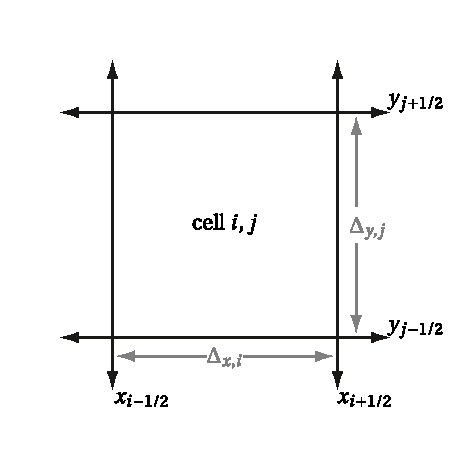
\includegraphics{cell-diagram}
  \caption{Diagram of cell $i,j$.}
  \label{fig:cellDiagram}
\end{figure}

To preserve particles, it's necessary that $F_T^y$ from cell $i,j$ is equal to
$F_B^y$ from cell $i,{j+1}$, and the same from the other directions.

%%%%%%%%%%%%%%%%%%%%%%%%%%%%%%%%%%%%%%%%%%%%%%%%%%%%%%%%%%%%%%%%%%%%%%%%%%%%%%%%
\section{Neglecting transverse diffusion}\label{sec:discreteDiag}

Perhaps the simplest way to discretize the anisotropic diffusion equation is by
neglecting the off-diagonal terms of the diffusion tensor that imply transverse
leakage.

In certain simple problems, this is not an approximation. As long as the
opacity is invariant with respect to one of the Cartesian coordinate system's
axes (see \S\ref{sec:eigenvectors}), the off-diagonal terms of $\Dtens$ are
zero, and the anisotropic Fick's law simplifies to:
\begin{equation*}
  \vec{F} = - \Dtens \vd \grad \phi
  = -
  \begin{bmatrix}
    D^{xx} & 0 \\
    0 & D^{yy}
  \end{bmatrix}
  \begin{bmatrix}
    \tpder{\phi}{x} \\
    \tpder{\phi}{y}
  \end{bmatrix}
  = 
  \begin{bmatrix}
    - D^{xx} \tpder{\phi}{x} \\
    - D^{yy} \tpder{\phi}{y}
  \end{bmatrix}
  \,.
\end{equation*}

Without loss of generality, we evaluate the net leakage from cell
$i,j$ through its right face:
\begin{align} \nonumber
  F_R^x &\equiv \frac{1}{\Delta_{y,j}} \int_{y_{j-1/2}}^{y_{j+1/2}}
  \vec{F}(x_{i+1/2}, y) \vd \vec{n}_R \ud y\,.
  \\
  \intertext{Substituting the anisotropic Fick's law,} \nonumber
  F_R^x &= - \frac{1}{\Delta_{y,j}} \int_{y_{j-1/2}}^{y_{j+1/2}}
  D_{i,j}^{xx} \pder{\phi}{x} \ud y \,.
  \\ 
  \intertext{Now we introduce a temporary cell-edge $\phi_{i+1/2}$ and
  approximate the partial derivative using a second-order finite difference:}
  \label{eq:diagFrx}
  F_R^x &\approx - 
  D_{i,j}^{xx} \frac{\phi_{i+1/2,j} - \phi_{i}}{\Delta_{x,i}/2} \,.
\end{align}
Evaluating the net leakage from cell $i+1,j$ through its left face by using the
cell-edged $\phi_{i+1/2}$ and finite difference approximation, we obtain
\begin{equation}\label{eq:diagFlx}
  F_{L,i+1,j}^x \approx - 
  D_{i+1,j}^{xx} \frac{\phi_{i+1,j} - \phi_{i+1/2}}{\Delta_{x,i+1}/2} \,.
\end{equation}
Scaling Eqs.~\eqref{eq:diagFrx} and~\eqref{eq:diagFlx} by $\Delta_x/(2 D^{xx})$
and adding them, we obtain
\begin{equation*}
  \frac{\Delta_{x_{i+1/2}}}{D_{i,j}^{xx}}F_R^x
 + \frac{\Delta_{x_{i+1/2}}}{D_{i+1,j}^{xx}}F_{L,i+1,j}^x
 = -(\phi_{i+1/2,j} - \phi_{i}) + -(\phi_{i+1,j} - \phi_{i+1/2})\,.
\end{equation*}
The cell-edged $\phi$ cancels out. Enforcing particle conservation by
setting $F_R^x = F_{L,i+1,j}^x$ yields the expression for the net leakage
through the right face of cell $i,j$:
\begin{equation}\label{eq:diagRight}
  F_R^x= -\frac{D^{xx}_{i+1/2,j}}{\Delta_{x,i+1/2}}
  \left( \phi_{i+1,j} - \phi_{i,j} \right)\,,
\end{equation}
where we have defined a harmonically averaged cell edge diffusion coefficient
and a half-edge width,
\begin{equation} \label{eq:cellEdgeDHarmonic}
  \frac{D^{xx}_{i+1/2,j}}{\Delta_{x,i+1/2}} \equiv \left[
  \frac12 \left( \frac{D^{xx}_{i,j}}{\Delta_{x,i}} \right)\inv
 + \frac12 \left( \frac{D^{xx}_{i+1,j}}{\Delta_{x,i+1}} \right)\inv
  \right]\inv\,.
\end{equation}
This is the standard relation between neighboring cells in the
cell-centered discretization scheme \cite{Dud1976}, except that in anisotropic
diffusion, leakage across the face normal to the $x$ axis takes the $D^{xx}$
component of the diffusion tensor.

Repeating the same procedure through the left, top, and bottom faces yield the
following similar equations:
\begin{align*}
  F_L^x &= -\frac{D^{xx}_{i-1/2,j}}{\Delta_{x,i-1/2}}
  \left( \phi_{i,j} - \phi_{i-1,j} \right)\,,
  \\
  F_T^y &= -\frac{D^{yy}_{i,j+1/2}}{\Delta_{y,j+1/2}}
  \left( \phi_{i,j+1} - \phi_{i,j} \right)\,,
  \\
  F_B^y &= -\frac{D^{yy}_{i,j-1/2}}{\Delta_{y,j-1/2}}
  \left( \phi_{i,j} - \phi_{i,j-1} \right)\,.
\end{align*}
Substituting these into Eq.~\eqref{eq:ssConservationDisc} relates the
cell-centered values of $\phi$ in the interior:
\begin{multline} \label{eq:diagConservation}
  \Delta_{x,i} \left(
  - \frac{D^{yy}_{i,j+1/2}}{\Delta_{y,j+1/2}} \left( \phi_{i,j+1} - \phi_{i,j}
    \right)
  + \frac{D^{yy}_{i,j-1/2}}{\Delta_{y,j-1/2}} \left( \phi_{i,j} - \phi_{i,j-1}
    \right)
  \right)
\\
+ \Delta_{y,j} \left(
  - \frac{D^{xx}_{i+1/2,j}}{\Delta_{x,i+1/2}} \left( \phi_{i+1,j} - \phi_{i,j}
    \right)
  + \frac{D^{xx}_{i-1/2,j}}{\Delta_{x,i-1/2}} \left( \phi_{i,j} - \phi_{i-1,j}
    \right)
  \right)
\\
+ \Delta_{x,i}\Delta_{y,j} \sigma_{a,i,j} \phi_{i,j}
= \Delta_{x,i}\Delta_{y,j} q_{i,j}\,.
\end{multline}
Rearranging shows the leakage terms to be part of a discretized Laplacian
operator.

When a cell has one or more face on an exterior boundary, the above relations
for $\vec{n}\vd \vec{F}$ are replaced by a discretized form of the boundary
condition, derived in \S\ref{sec:discreteBc}.

%%%%%%%%%%%%%%%%%%%%%%%%%%%%%%%%%%%%%%%%%%%%%%%%%%%%%%%%%%%%%%%%%%%%%%%%%%%%%%%%
\section{Gol'din-style discretization}

Anisotropic diffusion bears a superficial resemblance to the
Quasidiffusion (QD) method in that they both contain a tensor in their
approximation to the radiation flux. The crucial difference is in the placement
of the gradient operator $\grad$: steady-state AD uses the approximation
\begin{align*}
  \vec{F} &= - \Dtens \vd \grad \phi
  \\ 
  \intertext{whereas steady-state QD uses the approximation}
  \vec{F} &= - \frac{1}{\sigma} \grad \vd \Etens \phi\,.
\end{align*}
The presence of the tensor means that spatial discretizations for QD are
correspondingly more complex than standard diffusion. One discretization scheme,
developed by Gol'din \cite{Val2002}, is straightforward to derive and implement.

The Gol'din method is to introduce unknowns at both the cell centers and the
cell edges, integrate $\vec{F}\vd \vec{n}$ over half of a cell, approximating
it as a constant in that domain, and use
particle conservation to relate adjacent cells.

Now we apply Gol'din's method to the anisotropic diffusion equation. We begin
by integrating Eq.~\eqref{eq:anisotropicFicks2d} over the right half of the
cell (see Fig.~\ref{fig:goldinRight}),
\begin{figure}[htb]
  \centering
  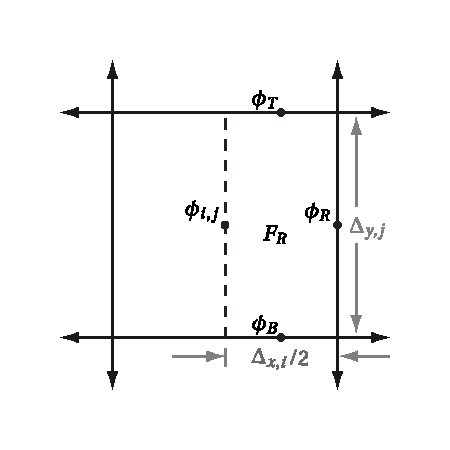
\includegraphics{goldin-righthalf}
  \caption{Right half of cell $i,j$.}
  \label{fig:goldinRight}
\end{figure}
evaluating the flux exiting the right face $F_R^x = \vec{F}\vd\vec{n}_R$.
\begin{align*}
\int_{y_{j-1/2}}^{y_{j+1/2}} \int_{x_{i}}^{x_{i+1/2}}
\vec{n}_R \vd \vec{F}
\ud x \ud y
&=
\int_{y_{j-1/2}}^{y_{j+1/2}} \int_{x_{i}}^{x_{i+1/2}}
-\vec{n}_R \vd \Dtens \vd \grad \phi
\ud x \ud y
\\
F_R^x \frac{\Delta_{x,i} \Delta_{y,j}}{2}
&=
-
\begin{bmatrix}
  1 & 0
\end{bmatrix}
\begin{bmatrix}
  D_{i,j}^{xx} & D_{i,j}^{yx} \\
  D_{i,j}^{xy} & D_{i,j}^{yy}
\end{bmatrix}
\int_{y_{j-1/2}}^{y_{j+1/2}} \int_{x_{i}}^{x_{i+1/2}}
\begin{bmatrix}
  \tpder{\phi}{x} \\
  \tpder{\phi}{y}
\end{bmatrix}
\ud x \ud y
\\
F_R^x \frac{\Delta_{x,i} \Delta_{y,j}}{2}
&=
-
\begin{bmatrix}
  D_{i,j}^{xx} & D_{i,j}^{yx}
\end{bmatrix}
\begin{bmatrix}
  \left( \phi_R - \phi_{i,j} \right) \Delta_{y,j} \\
  \left( \phi_T - \phi_B \right) \Delta_{x,i} / 2
\end{bmatrix}
\ud x \ud y
\\
F_R^x
&= 
- D_{i,j}^{xx} \frac{\phi_R - \phi_{i,j}}{ \Delta_{x,i} / 2}
- D_{i,j}^{yx} \frac{\phi_T - \phi_B}{ \Delta_{y,j} }\ \,.
\end{align*}
Performing the same procedure for the left side, we obtain
\begin{align*}
\int_{y_{j-1/2}}^{y_{j+1/2}} \int_{x_{i-1/2}}^{x_{i}}
\vec{n}_L \vd \vec{F}
\ud x \ud y
&=
\int_{y_{j-1/2}}^{y_{j+1/2}} \int_{x_{i-1/2}}^{x_{i}}
-\vec{n}_L \vd \Dtens \vd \grad \phi
\ud x \ud y
\\
-F_L^x \frac{\Delta_{x,i} \Delta_{y,j}}{2}
&=
-
\begin{bmatrix}
  -1 & 0
\end{bmatrix}
\begin{bmatrix}
  D_{i,j}^{xx} & D_{i,j}^{yx} \\
  D_{i,j}^{xy} & D_{i,j}^{yy}
\end{bmatrix}
\int_{y_{j-1/2}}^{y_{j+1/2}} \int_{x_{i-1/2}}^{x_{i}}
\begin{bmatrix}
  \tpder{\phi}{x} \\
  \tpder{\phi}{y}
\end{bmatrix}
\ud x \ud y
\\
F_L^x \frac{\Delta_{x,i} \Delta_{y,j}}{2}
&=
-
\begin{bmatrix}
  D_{i,j}^{xx} & D_{i,j}^{yx}
\end{bmatrix}
\begin{bmatrix}
  \left( \phi_{i,j} - \phi_L \right) \Delta_{y,j} \\
  \left( \phi_T - \phi_B \right) \Delta_{x,i} / 2
\end{bmatrix}
\ud x \ud y
\\
F_L^x
&= 
- D_{i,j}^{xx} \frac{\phi_{i,j} - \phi_L}{ \Delta_{x,i} / 2}
- D_{i,j}^{yx} \frac{\phi_T - \phi_B}{ \Delta_{y,j} }\,.
\end{align*}

Rotating the coordinate system by swapping $x\leftrightarrow y$, $T
\leftrightarrow R$, $B \leftrightarrow L$, and $i \leftrightarrow j$, we have
corresponding equations for the top and bottom leakage terms:
\begin{align*}
F_T^y
&= 
- D_{i,j}^{yy} \frac{\phi_T - \phi_{i,j}}{ \Delta_{y,j} / 2}
- D_{i,j}^{xy} \frac{\phi_R - \phi_L}{ \Delta_{x,i} }\,,
\\  
F_B^y
&= 
- D_{i,j}^{yy} \frac{\phi_{i,j} - \phi_B}{ \Delta_{y,j} / 2}
- D_{i,j}^{xy} \frac{\phi_R - \phi_L}{ \Delta_{x,i} }\,.
\end{align*}

At each interior face, we demand that the scalar intensity $\phi$ is continuous,
i.e.,
\begin{equation*}
  \phi_{R,i,j} = \phi_{L,i+1,j} \equiv \phi_{i+1/2,j}\,.
\end{equation*}
Substituting these definitions and the net leakage expressions into the
conservation equation~\eqref{eq:ssConservationDisc}, we obtain $I\times J$
equations,
\begin{multline*}
- \Delta_{x,i} D_{i,j}^{yy}\frac{\phi_{i,j+1/2} - \phi_{i,j}}{\Delta_{y,j} / 2}
- \Delta_{x,i} D_{i,j}^{xy}\frac{\phi_{i+1/2,j} - \phi_{i-1/2,j}}{\Delta_{x,i} }
\\
+ \Delta_{x,i} D_{i,j}^{yy}\frac{\phi_{i,j} - \phi_{i,j-1/2}}{\Delta_{y,j} / 2}
+ \Delta_{x,i} D_{i,j}^{xy}\frac{\phi_{i+1/2,j} - \phi_{i-1/2,j}}{\Delta_{x,i} }
\\
- \Delta_{y,j} D_{i,j}^{xx}\frac{\phi_{i+1/2,j} - \phi_{i,j}}{\Delta_{x,i} / 2}
- \Delta_{y,j} D_{i,j}^{yx}\frac{\phi_{i,j+1/2} - \phi_{i,j-1/2}}{\Delta_{y,j} }
\\
+ \Delta_{y,j} D_{i,j}^{xx}\frac{\phi_{i,j} - \phi_{i-1/2,j}}{\Delta_{x,i} / 2}
+ \Delta_{y,j} D_{i,j}^{yx}\frac{\phi_{i,j+1/2} - \phi_{i,j-1/2}}{\Delta_{y,j} }
\\
+ \Delta_{x,i}\Delta_{y,j} \sigma_{a,i,j} \phi_{i,j}
= \Delta_{x,i}\Delta_{y,j} q_{i,j}\,.
\end{multline*}
The transverse leakage terms cancel, leaving
\begin{multline*}
\phi_{i,j} \left(
   4 D_{i,j}^{xx} \frac{\Delta_{y,j}}{\Delta_{x,i}}
 + 4 D_{i,j}^{yy} \frac{\Delta_{x,i}}{\Delta_{y,j}}
 + \Delta_{x,i}\Delta_{y,j} \sigma_{a,i,j} \right)
 \\
- 2 D_{i,j}^{xx} \frac{\Delta_{y,j}}{\Delta_{x,i}}
  \left( \phi_{i+1/2,j} + \phi_{i-1/2,j} \right)
- 2 D_{i,j}^{yy} \frac{\Delta_{x,i}}{\Delta_{y,j}}
  \left( \phi_{i,j+1/2} + \phi_{i,j-1/2} \right)
\\= \Delta_{x,i}\Delta_{y,j} q_{i,j}\,.
\end{multline*}

To complete the equations for the Gol'din discretization, we enforce continuity
of the radiation flux on interior faces, setting $F_{T,i,j}^y = F_{B,i,j+1}^y$
and $F_{R,i,j}^x = F_{L,i+1,j}^x$, to yield the relations
\begin{equation*}
- D_{i,j}^{yy} \frac{\phi_{i,j+1/2} - \phi_{i,j}}{ \Delta_{y,j} / 2}
- D_{i,j}^{xy} \frac{\phi_{i+1/2,j} - \phi_{i-1/2,j}}{ \Delta_{x,i} }
=
- D_{i,j+1}^{yy} \frac{\phi_{i,j+1} - \phi_{i,j+1/2}}{ \Delta_{y,j} / 2}
- D_{i,j+1}^{xy} \frac{\phi_{i+1/2,j+1} - \phi_{i-1/2,j+1}}{ \Delta_{x,i} }\,.
\end{equation*}
and
\begin{equation*}
- D_{i,j}^{xx} \frac{\phi_{i+1/2,j} - \phi_{i,j}}{ \Delta_{x,i} / 2}
- D_{i,j}^{yx} \frac{\phi_{i,j+1/2} - \phi_{i,j-1/2}}{ \Delta_{y,j} }
=
- D_{i+1,j}^{xx} \frac{\phi_{i+1,j} - \phi_{i,j}}{ \Delta_{x,i} / 2}
- D_{i+1,j}^{yx} \frac{\phi_{i+1,j+1/2} - \phi_{i+1,j-1/2}}{ \Delta_{y,j} }\,.
\end{equation*}

Note that, if $D^{xy} = D^{yx}=0$, the cell-edged $\phi$ can be eliminated, and
Gol'din's method will reduce to the simple cell-centered difference scheme of
\S\ref{sec:discreteDiag}.

%%%%%%%%%%%%%%%%%%%%%%%%%%%%%%%%%%%%%%%%%%%%%%%%%%%%%%%%%%%%%%%%%%%%%%%%%%%%%%%%
\section{Nine-point stencil}

Fig.~\ref{fig:cellAnisoLeakage} shows the leakage out of cell $i,j$ through the
right face.
\begin{figure}[htb]
  \centering
  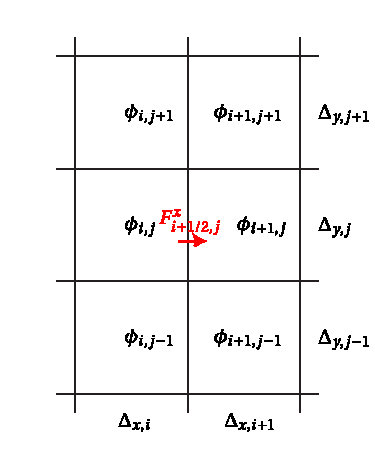
\includegraphics{cell-leakage-right}
  \caption{Diagram showing the radiation exiting interior cell $i,j$ through the
  right face.}
  \label{fig:cellAnisoLeakage}
\end{figure}
We evaluate the face-averaged normal component of the flux,
$F_{i+1/2,j}^x \equiv \int_{y_{j-1/2}}^{y_{j+1/2}} \vec{F} \vd \vec{n} \ud
y$, from both cell $i,j$ and cell $i+1,j$, and set them equal to each other.
Solving for $F_{i+1/2,j}^x$ gives
\begin{equation} \label{eq:cellAnisoFlux}
  F_{i+1/2,j}^{x} \approx
  - \frac{D^{xx}_{i+1/2,j}}{\Delta_{x,i+1/2}}
  \left[ 
    \left( \phi_{i+1,j} - \phi_{i,j} \right)
  + \frac{D^{xy}_{i,j}/D^{xx}_{i,j}}{2/\Delta_{x,i}}
    \pder{\phi}{y} \Bigg|_{x_{i+1/2}^-}
  + \frac{D^{xy}_{i+1,j}/D^{xx}_{i+1,j}}{2/\Delta_{x,i+1}}
    \pder{\phi}{y} \Bigg|_{x_{i+1/2}^+}
  \right]
\end{equation}
where $\tpder{\phi}{y} |_{x_{i+1/2}^-}$ is the transverse derivative of
$\phi$ on the left side of the face, and $\tpder{\phi}{y} |_{x_{i+1/2}^+}$ is
the transverse derivative as viewed from the right side of the face.
The harmonic-averaged diffusion coefficient is
\begin{equation} \label{eq:cellEdgeDHarmonic}
  \frac{D^{xx}_{i+1/2,j}}{\Delta_{x,i+1/2}} \equiv \left[
  \frac12 \left( \frac{D^{xx}_{i,j}}{\Delta_{x,i}} \right)\inv
 + \frac12 \left( \frac{D^{xx}_{i+1,j}}{\Delta_{x,i+1}} \right)\inv
  \right]\inv\,.
\end{equation}

If $D^{xy}$ were zero for both cells, and $D^{xx}=D^{yy}$,
Eq.~\eqref{eq:cellAnisoFlux} would reduce to
the standard cell-centered finite difference discretization so well known to
nuclear engineering students.

Now, in our first nine-point stencil, we approximated
\begin{equation*}
  \pder{\phi}{y} \Bigg|_{x_{i+1/2}^-} \approx \frac{\phi_{i,j+1} -
  \phi_{i,j-1}}{\tfrac12 \Delta_{y,j+1} + \Delta_{y,j} + \tfrac12
  \Delta_{y,j-1}}
\end{equation*}
in the interior of the problem and discarded the term near the boundaries. (The 
$\tpder{\phi}{y} |_{x_{i+1/2}^+}$ term is the same but replacing $i\to i+1$.)
An improvement is to approximate the case on the top boundary with
\begin{equation*}
  \pder{\phi}{y} \Bigg|_{x_{i+1/2}^-} \approx \frac{\phi_{i,j} -
  \phi_{i,j-1}}{\tfrac12 \Delta_{y,j} + \tfrac12 \Delta_{y,j-1} }
\end{equation*}
and the case on the bottom boundary with 
\begin{equation*}
  \pder{\phi}{y} \Bigg|_{x_{i+1/2}^-} \approx \frac{\phi_{i,j+1} -
  \phi_{i,j}}{\tfrac12 \Delta_{y,j+1} + \tfrac12 \Delta_{y,j} }
\end{equation*}

We can also approximate this derivative with approximate cell-edge values. In
the finite difference method, an intermediate cell-edge $\phi$ helps represent
the slope normal to the edge. It is eliminated in the process of finding
$\vec{F}\vd\vec{n}$, but if there is no transverse term, it is possible to
solve for the cell-edge $\phi$ in terms of the two cell-centered $\phi$. Let us
consider the finite difference approximation coupling two cells:
\begin{equation*}
  F = - D_0 \frac{\phi_{1/2} - \phi_0}{\Delta_0/2}
  \qquad\text{and}\qquad
  F = - D_1 \frac{\phi_{1} - \phi_{1/2}}{\Delta_1/2}\,.
\end{equation*}
Multiplying the left equation by $\Delta_0 / D_0$ and the right equation by
$\Delta_1 / D_1$,
\begin{equation*}
  -\frac{\Delta_0/2}{D_0 } F = \phi_{1/2} - \phi_0
  \qquad\text{and}\qquad
  -\frac{\Delta_1/2}{D_1 } F = \phi_{1} - \phi_{1/2}
\end{equation*}
adding them eliminates gives the standard finite-difference approximation for
$F$,
\begin{equation*}
  F = - \left( \frac{\Delta_0/2}{D_0 } + \frac{\Delta_1/2}{D_1 } \right)\inv
  \left( \phi_1 - \phi_0 \right),
\end{equation*}
and subtracting the second from the first gives
\begin{equation*}
 -\frac{\Delta_0/2}{D_0 }F + \frac{\Delta_1/2}{D_1 } F
 = 2 \phi_{1/2}-(\phi_0+\phi_1)\,.
\end{equation*}
Defining $ d_i \equiv \frac{\Delta_i}{D_i}$ for $i=0,1$ for brevity, then
\begin{equation*}
  \frac12 F (d_1 - d_0)
 = 2 \phi_{1/2}-(\phi_0+\phi_1)
  \qquad\text{and}\qquad
 F = -2\left( d_1 + d_0 \right)\inv (\phi_1 - \phi_0)\,.
\end{equation*}
Substituting $F$ into the left equation,
\begin{align*}
  \left( d_1 + d_0 \right)\inv\left(d_1 - d_0\right) (\phi_1 - \phi_0)
  &= 2 \phi_{1/2}-(\phi_0+\phi_1)
  \\
 \frac12 \left[ 1 - \frac{d_1 - d_0}{d_1 + d_0} \right] \phi_1
+ \frac12 \left[ 1 + \frac{d_1 - d_0}{d_1 + d_0} \right] \phi_0
 &= \phi_{1/2}
  \\
 \frac{d_0}{d_1 + d_0} \phi_1
+ \frac{d_1}{d_1 + d_0} \phi_0
 &= \phi_{1/2}\,.
\end{align*}

For our case in anisotropic diffusion, we want to approximate 
\begin{equation*}
  \pder{\phi}{y} \Bigg|_{x_{i+1/2}^-} \approx \frac{\phi_{i,j+1/2} -
  \phi_{i,j-1/2}}{\Delta_{y,j}} \,.
\end{equation*}
In evaluating these cell-edge $\phi$ we neglect the transverse leakage (as
leaving them in would add unknowns on more cell faces) and apply the previous
result:
\begin{equation*}
  \phi_{i,j+1/2} \approx
  \frac{D_{i,j}^{yy} / \Delta_{y,j}}{D_{i,j+1}^{yy} / \Delta_{y,j+1} +
  D_{i,j}^{yy} / \Delta_{y,j}} \phi_{i,j+1}
+ \frac{D_{i,j+1}^{yy} / \Delta_{y,j+1}}{D_{i,j+1}^{yy} / \Delta_{y,j+1} +
D_{i,j}^{yy} / \Delta_{y,j}} \phi_{i,j} \,.
\end{equation*}
Subtracting one from the $j$ indices gives the corresponding equation for the
bottom face:
\begin{equation*}
  \phi_{i,j-1/2} \approx
  \frac{D_{i,j-1}^{yy} / \Delta_{y,j-1}}{D_{i,j}^{yy} / \Delta_{y,j} +
  D_{i,j-1}^{yy} / \Delta_{y,j-1}} \phi_{i,j}
+ \frac{D_{i,j}^{yy} / \Delta_{y,j}}{D_{i,j}^{yy} / \Delta_{y,j} +
D_{i,j-1}^{yy} / \Delta_{y,j-1}} \phi_{i,j-1} \,.
\end{equation*}
If cell $i,j$ is in the interior, 
\begin{equation*}
  \pder{\phi}{y} \Bigg|_{x_{i+1/2}^-} \approx \frac{\phi_{i,j+1/2} -
  \phi_{i,j-1/2}}{\Delta_{y,j}} \,,
\end{equation*}
or if it is on the top boundary,
\begin{equation*}
  \pder{\phi}{y} \Bigg|_{x_{i+1/2}^-} \approx \frac{\phi_{i,j} -
  \phi_{i,j-1/2}}{\Delta_{y,j} / 2} \,,
\end{equation*}
or if it is on the bottom boundary,
\begin{equation*}
  \pder{\phi}{y} \Bigg|_{x_{i+1/2}^-} \approx \frac{\phi_{i,j+1/2} -
  \phi_{i,j}}{\Delta_{y,j} / 2} \,.
\end{equation*}

If the anisotropic diffusion coefficients are homogeneous and the grid is
uniform, this expression for $\tpder{\phi}{y}$ is exactly equivalent to the
simpler one.

\begin{figure}[htb]
  \centering
  %\hspace{-.6in}
  \subfigure[Diagonal-only anisotropic]{
  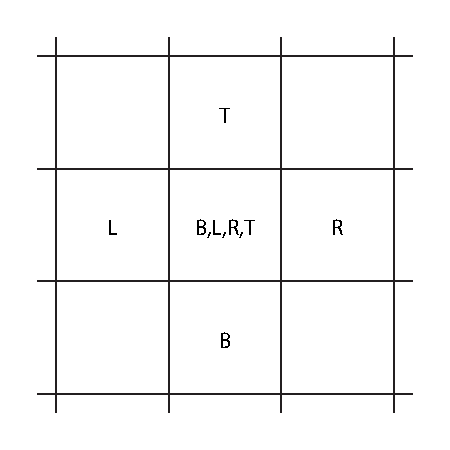
\includegraphics{diaganiso-leakage-terms}
  }
  %\hspace{-.2in}
  \subfigure[Cell anisotropic]{
  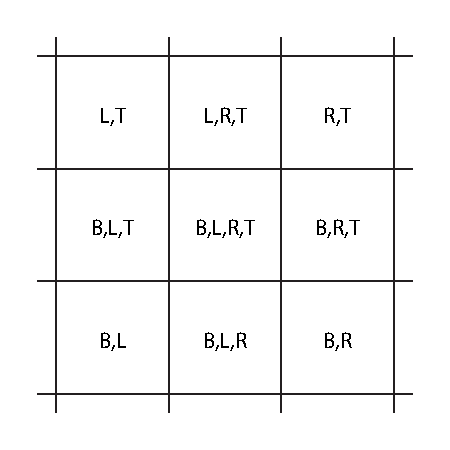
\includegraphics{cellaniso-leakage-terms}
  }
  %\hspace{-.6in}
  \caption{Stencils for $- \grad \vd \Dtens \grad \phi$ showing contribution
  from the leakage terms of each face of the center cell.}
  \label{fig:anisoStencils}
\end{figure}

%%%%%%%%%%%%%%%%%%%%%%%%%%%%%%%%%%%%%%%%%%%%%%%%%%%%%%%%%%%%%%%%%%%%%%%%%%%%%%%%
\section{Incident boundary conditions} \label{sec:discreteBc}
(Do I show how to write boundary conditions for these schemes? I am sure that it
has been done before.)

For the cell-centered and staggered-mesh schemes of AD and \APone, respectively,
we desire boundary conditions that relate cell-edge leakage $\vec{n}\vd\vec{F}$
to cell-centered scalar intensity $\phi$.

A reflecting boundary condition for the transport equation translates to an
``insulating'' boundary condition in the low-order diffusion equations. There
is zero net leakage at the exterior face, $\vec{n}\vd\vec{F}=0$.

Incident boundary conditions are more complicated.
We will take the general \Pone\ boundary condition case:
\begin{subequations} \label{eqs:discreteBc}
\begin{equation} \label{eq:discreteBcGeneral}
  \beta = \phi - \alpha\vec{n}\vd \vec{F}
\end{equation}
with
\begin{equation} \label{eq:discreteBcGeneralF}
  \vec{n} \vd \vec{F}
  = - \vec{n}\vd \Dtens \vd \grad \phi
  + \gamma \vec{n}\vd \Dtens \vd \vec{F}^{i}\,.
\end{equation}
\end{subequations}
Here, $\beta$ is the source term that results from a positive incident
radiation source, $\alpha$ is the extrapolation distance, and $\gamma$ is
related to the geometry but is zero for diffusion.

\begin{table}[htb]
  \centering
  \begin{tabular}{rccc}
\toprule
& $\beta$
& $\alpha$
& $\gamma$
\\ \midrule
2-D Marshak AD
& $4 F^-$
& $2/3$
& $0$
\\
2-D Transport AD
& $2\int_{\vec{\Omega}\vd \vec{n} < 0} W I^b \ud\Omega$
& $0.7104$
& $0$
\\
Flatland Marshak AD
& $\pi F^-$
& $\pi/2$
& $0$
\\
2-D Marshak \APone
& $4 F^-$
& $2/3$
& $3/c \Delta_t$
\\
Flatland Marshak \APone
& $\pi F^-$
& $\pi/2$
& $2/c \Delta_t$
\\ \bottomrule
  \end{tabular}
  \caption{Coefficients for the discretized boundary conditions.}
  \label{tab:discreteBcCoeffs}
\end{table}

First, we note that, in accordance with the derivation in \S\ref{sec:zeta}, the
off-diagonal components of $\Dtens$ are zero, so we do not need to consider
transverse leakage at the boundary face. Evaluating
Eq.~\eqref{eq:discreteBcGeneralF} at a cell $i,j$ on the right boundary, and
introducing a temporary cell-edge $\phi_{i+1/2,j}$ with which we approximate the
gradient,
\begin{align} \nonumber
  F_R^y 
  &= - D_{i,j}^{xx} \frac{\phi_{i+1/2,j} - \phi_{i,j}}{\Delta_{x,i} / 2}
  + \gamma D_{i,j}^{xx} F_{i+1/2,j}^{i} \,.
\\ 
\intertext{For brevity, we write this as}
\label{eq:discreteBcFBrief}
  F
  &= - D \frac{\phi^* - \phi}{\Delta / 2}
  + \gamma D \hat F \,,
\end{align}
where $\phi^*$ is the cell-edge scalar intensity, and $\hat F$ is the initial
condition for the net radiation flux on the right face.

Substituting into Eq.~\eqref{eq:discreteBcGeneral}, which at the right boundary
is
\begin{equation*}
  \beta
  = \phi_{i+1/2,j}
  - \alpha F_R^y
  = \phi^* - \alpha F \,,
\end{equation*}
we obtain the relation
\begin{equation*}
  \beta
  = \phi^*
  + \alpha D \frac{\phi^* - \phi}{\Delta / 2}
  - \alpha \gamma D \hat F \,.
\end{equation*}
A little manipulation gives
\begin{equation*}
  \phi^* = \left( 1 + \frac{\alpha D}{\Delta/2} \right)\inv \left( \beta
  + \frac{\alpha D}{\Delta/2} \phi + \alpha \gamma D \hat F
  \right)\,.
\end{equation*}
We use this result to eliminate $\phi^*$ from Eq.~\eqref{eq:discreteBcFBrief}:
\begin{align*}
  F
  &= - \frac{D}{\Delta / 2} \phi^* + \frac{D}{\Delta / 2}\phi
  + \gamma D \hat F
  \\
  F
  &= -\left(  \frac{\Delta}{2 D} + \alpha\right)\inv
  \left( \beta
  + \frac{2 \alpha D}{\Delta} \phi + \alpha \gamma D \hat F
  \right)
  + \frac{D}{\Delta / 2}\phi
  + \gamma D \hat F
  \\
  F
  &= -\left(  \frac{\Delta}{2 D} + \alpha\right)\inv \beta
  + \left[ 1 - \left(1 + \frac{\Delta}{2 \alpha D} \right)\inv \right]
  \left( \frac{2D}{\Delta} \phi + \gamma D \hat F \right) \,.
\end{align*}
Because of potential machine precision error for optically thin cells
($\eps \equiv \Delta / D$), it is better to implement
\begin{equation*}
  \left[ 1 - \left( 1 + \frac{\Delta}{2 \alpha D} \right)\inv  \right]
  \to \left[ \frac{\frac{\Delta}{2 \alpha D}}{1 + \frac{\Delta}{2 \alpha D}}
  \right]
  = \left[ \frac{\Delta}{2 \alpha D + \Delta} \right]\,.
\end{equation*}
The equation for the net leakage out of a boundary cell on the right is
therefore
\begin{equation} \label{eq:discreteBcRight}
  F
  = -\left(  \frac{\Delta}{2 D} + \alpha\right)\inv \beta
  + \left[ 2 \alpha D + \Delta \right]\inv
  \left( 2D \phi + \gamma \Delta D \hat F \right) \,.
\end{equation}
This equation is also valid (after redefining $D=D^{yy}$, etc.) on the top
boundary, because there the sign of the face normal vector is also positive, and
the gradient is approximated in the same way.

On the left and bottom boundaries, $\vec{n}\vd \vec{F}$ and the approximation to
$\grad \phi$ have changes in sign. With diffusion ($\gamma=0$), the two sign
changes cancel, but the extra term in the \APone\ equation for $\vec{F}$ means
that one of the signs is different from Eq.~\eqref{eq:discreteBcRight}. The net
leakage term in Eq.~\eqref{eq:discreteBcGeneralF} for the left boundary takes on
a negative sign because $\vec{n}=- \vec{n}_x$, and the finite difference
approximation to $\grad \phi$ is different:
\begin{align} \nonumber
  \vec{F}\vd \vec{n} &= -F_L^x 
  \\
  &= (-1) \left(
  - D_{i,j}^{xx} \frac{\phi_{i,j} - \phi_{i-1/2,j}}{\Delta_{x,i} / 2}
  + \gamma D_{i,j}^{xx} F_{i+1/2,j}^{i}\right) \,,
\\ 
\intertext{or in brief form,}
\nonumber
F &= D \frac{\phi^* - \phi}{\Delta / 2} - \gamma D \hat F \,.
\end{align}
The term with $\hat F$ has a different sign from the corresponding term on a
positive boundary. Substituting this expression into
Eq.~\eqref{eq:discreteBcGeneral} gives
\begin{equation*}
  \beta = \phi^*
  + \alpha D \frac{\phi^* - \phi}{\Delta / 2} + \alpha \gamma D \hat F \,.
\end{equation*}
Eliminating $\phi^*$ from the previous equation gives the net current on the
left face:
\begin{equation*}
  F
  = -\left(  \frac{\Delta}{2 D} + \alpha\right)\inv \beta
  + \left[ 2 \alpha D + \Delta \right]\inv
  \left( 2D \phi - \gamma \Delta D \hat F \right) \,.
\end{equation*}
This equation, valid for bottom and left boundaries, has the same sign as the
top and right for the $\phi$ term but the opposite sign for the $\hat F$ term.



% !TEX root = _individual/simpleNumericalResults.tex

%%%%%%%%%%%%%%%%%%%%%%%%%%%%%%%%%%%%%%%%%%%%%%%%%%%%%%%%%%%%%%%%%%%%%%%%%%%%%%%%
\chapter{Numerical Results: Test Problems}\label{chap:simpleNumericalResults}


%%%%%%%%%%%%%%%%%%%%%%%%%%%%%%%%%%%%%%%%%%%%%%%%%%%%%%%%%%%%%%%%%%%%%%%%%%%%%%%%
\section{Discretization error}

\subsection{Low-order spatial discretization: manufactured solutions}

\begin{figure}[htb]
  \centering\small
  % GNUPLOT: LaTeX picture with Postscript
\begingroup
  \makeatletter
  \providecommand\color[2][]{%
    \GenericError{(gnuplot) \space\space\space\@spaces}{%
      Package color not loaded in conjunction with
      terminal option `colourtext'%
    }{See the gnuplot documentation for explanation.%
    }{Either use 'blacktext' in gnuplot or load the package
      color.sty in LaTeX.}%
    \renewcommand\color[2][]{}%
  }%
  \providecommand\includegraphics[2][]{%
    \GenericError{(gnuplot) \space\space\space\@spaces}{%
      Package graphicx or graphics not loaded%
    }{See the gnuplot documentation for explanation.%
    }{The gnuplot epslatex terminal needs graphicx.sty or graphics.sty.}%
    \renewcommand\includegraphics[2][]{}%
  }%
  \providecommand\rotatebox[2]{#2}%
  \@ifundefined{ifGPcolor}{%
    \newif\ifGPcolor
    \GPcolortrue
  }{}%
  \@ifundefined{ifGPblacktext}{%
    \newif\ifGPblacktext
    \GPblacktexttrue
  }{}%
  % define a \g@addto@macro without @ in the name:
  \let\gplgaddtomacro\g@addto@macro
  % define empty templates for all commands taking text:
  \gdef\gplbacktext{}%
  \gdef\gplfronttext{}%
  \makeatother
  \ifGPblacktext
    % no textcolor at all
    \def\colorrgb#1{}%
    \def\colorgray#1{}%
  \else
    % gray or color?
    \ifGPcolor
      \def\colorrgb#1{\color[rgb]{#1}}%
      \def\colorgray#1{\color[gray]{#1}}%
      \expandafter\def\csname LTw\endcsname{\color{white}}%
      \expandafter\def\csname LTb\endcsname{\color{black}}%
      \expandafter\def\csname LTa\endcsname{\color{black}}%
      \expandafter\def\csname LT0\endcsname{\color[rgb]{1,0,0}}%
      \expandafter\def\csname LT1\endcsname{\color[rgb]{0,1,0}}%
      \expandafter\def\csname LT2\endcsname{\color[rgb]{0,0,1}}%
      \expandafter\def\csname LT3\endcsname{\color[rgb]{1,0,1}}%
      \expandafter\def\csname LT4\endcsname{\color[rgb]{0,1,1}}%
      \expandafter\def\csname LT5\endcsname{\color[rgb]{1,1,0}}%
      \expandafter\def\csname LT6\endcsname{\color[rgb]{0,0,0}}%
      \expandafter\def\csname LT7\endcsname{\color[rgb]{1,0.3,0}}%
      \expandafter\def\csname LT8\endcsname{\color[rgb]{0.5,0.5,0.5}}%
    \else
      % gray
      \def\colorrgb#1{\color{black}}%
      \def\colorgray#1{\color[gray]{#1}}%
      \expandafter\def\csname LTw\endcsname{\color{white}}%
      \expandafter\def\csname LTb\endcsname{\color{black}}%
      \expandafter\def\csname LTa\endcsname{\color{black}}%
      \expandafter\def\csname LT0\endcsname{\color{black}}%
      \expandafter\def\csname LT1\endcsname{\color{black}}%
      \expandafter\def\csname LT2\endcsname{\color{black}}%
      \expandafter\def\csname LT3\endcsname{\color{black}}%
      \expandafter\def\csname LT4\endcsname{\color{black}}%
      \expandafter\def\csname LT5\endcsname{\color{black}}%
      \expandafter\def\csname LT6\endcsname{\color{black}}%
      \expandafter\def\csname LT7\endcsname{\color{black}}%
      \expandafter\def\csname LT8\endcsname{\color{black}}%
    \fi
  \fi
  \setlength{\unitlength}{0.0500bp}%
  \begin{picture}(5400.00,4320.00)%
    \gplgaddtomacro\gplbacktext{%
      \csname LTb\endcsname%
      \put(1020,640){\makebox(0,0)[r]{\strut{} $10^{-7}$}}%
      \put(1020,1131){\makebox(0,0)[r]{\strut{} $10^{-6}$}}%
      \put(1020,1623){\makebox(0,0)[r]{\strut{} $10^{-5}$}}%
      \put(1020,2114){\makebox(0,0)[r]{\strut{} 0.0001}}%
      \put(1020,2605){\makebox(0,0)[r]{\strut{} 0.001}}%
      \put(1020,3096){\makebox(0,0)[r]{\strut{} 0.01}}%
      \put(1020,3588){\makebox(0,0)[r]{\strut{} 0.1}}%
      \put(1020,4079){\makebox(0,0)[r]{\strut{} 1}}%
      \put(1140,440){\makebox(0,0){\strut{} 0.01}}%
      \put(2585,440){\makebox(0,0){\strut{} 0.1}}%
      \put(4029,440){\makebox(0,0){\strut{} 1}}%
      \put(200,2359){\rotatebox{-270}{\makebox(0,0){\strut{}Absolute error}}}%
      \put(3089,140){\makebox(0,0){\strut{}$\Delta_x$}}%
    }%
    \gplgaddtomacro\gplfronttext{%
      \csname LTb\endcsname%
      \put(4136,1403){\makebox(0,0)[r]{\strut{}Gol'din}}%
      \csname LTb\endcsname%
      \put(4136,1203){\makebox(0,0)[r]{\strut{}9-point}}%
      \csname LTb\endcsname%
      \put(4136,1003){\makebox(0,0)[r]{\strut{}9-point$*$}}%
      \csname LTb\endcsname%
      \put(4136,803){\makebox(0,0)[r]{\strut{}Diagonal}}%
    }%
    \gplbacktext
    \put(0,0){\includegraphics{/Users/seth/_thesis/figures/manufactured/convergence-multisolve-diag/convergence-multisolve-diag.pdf}}%
    \gplfronttext
  \end{picture}%
\endgroup

  \caption[Solution error (absolute volume-weighted 2-norm) in the
  finite difference discretization schemes.]{Solution error (absolute
  volume-weighted 2-norm) in the finite difference discretization schemes. The
  slopes of $\Delta_x^{2}$, $\Delta_x^{1.5}$, and
  $\Delta_x$, respectively.}
  \label{fig:manuConvergence}
\end{figure}

\begin{figure}[htb]
  \centering
  \includegraphics{manufactured/offdiag-contours}
  \caption[Solution contours for the manufactured solutions test.]{
  Solution contours for the manufactured solutions test. The red dashed line is
  the Diagonal scheme, the blue dashed line is the Gol'din scheme, cyan and green
  are the nine-point schemes, and the thin black line is the analytic solution.}
  \label{fig:manuSolution}
\end{figure}

\subsection{Transport discretization}

%%%%%%%%%%%%%%%%%%%%%%%%%%%%%%%%%%%%%%%%%%%%%%%%%%%%%%%%%%%%%%%%%%%%%%%%%%%%%%%%
\section{Flatland boundary conditions}

\begin{table}[htb]
  \centering
  \begin{tabular}{ccc}
\toprule
    Distribution & 1-D & Flatland
\\ \midrule
Isotropic & $I(\mu) = \frac{1}{2}$ & $I(\theta) = \frac{\pi}{2}$
\\
Normal & $I(\mu) = \delta(\mu-1)$ & $I(\theta) = \delta(\theta-\pi/2)$
\\
Grazing & $I(\mu) = \delta(\mu-0.1)$ & $I(\theta) = \delta(\theta-\sin\inv.1)$
\\ \bottomrule
  \end{tabular}
  \caption{Angular distributions used in boundary condition tests.}
  \label{tab:angularDistributions}
\end{table}

As a test problem, we consider a homogeneous flatland problem with a
total cross section $\sigma=1$ and scattering ratio $c=0.99$. It lives on the
domain $0 \le x \le 2$, $0 \le y \le 10$, with reflecting boundaries on the left,
right, and top sides. The bottom side has a specified boundary
condition with unit incident current, and we consider three different angular
distributions.

The first distribution is isotropic, $\psi^b(\theta) = \frac{1}{2}$. The second
is a normally incident flux, with all particles entering
perpendicular to the surface, $\psi^b(\theta) = \delta(\theta -
\frac{\pi}{2})$. The third incident distribution is at a grazing angle, with 
$\psi^b(\theta) = 10 \delta(\theta - \sin^{-1}.1)$.
These are the same angular distributions used in a boundary matching analysis
in \cite{Dav2006}.

Figure~\ref{fig:isotropic} shows a line-out of the scalar flux $\phi_0$ along
$x=1$ for an isotropic incident source. Because the left-hand sides of
Eqs.~\eqref{eq:flatlandDiffusionMarshak} and~\eqref{eq:flatlandDiffusionVarBc} are the same, the
differences in the solution are only due to the slightly different
extrapolation distance.

However, for the highly anisotropic normal and grazing cases,
Figs.~\ref{fig:delta} and~\ref{fig:grazing}, the Marshak boundary fails to
limit to the transport solution outside of the boundary layer. As
expected, the variational boundary condition does a much better job of
approximating the interior solution of the scalar flux.

\begin{figure}[htb!]
  \centering\small
  \hspace{-.5in}
  % GNUPLOT: LaTeX picture with Postscript
\begingroup
  \makeatletter
  \providecommand\color[2][]{%
    \GenericError{(gnuplot) \space\space\space\@spaces}{%
      Package color not loaded in conjunction with
      terminal option `colourtext'%
    }{See the gnuplot documentation for explanation.%
    }{Either use 'blacktext' in gnuplot or load the package
      color.sty in LaTeX.}%
    \renewcommand\color[2][]{}%
  }%
  \providecommand\includegraphics[2][]{%
    \GenericError{(gnuplot) \space\space\space\@spaces}{%
      Package graphicx or graphics not loaded%
    }{See the gnuplot documentation for explanation.%
    }{The gnuplot epslatex terminal needs graphicx.sty or graphics.sty.}%
    \renewcommand\includegraphics[2][]{}%
  }%
  \providecommand\rotatebox[2]{#2}%
  \@ifundefined{ifGPcolor}{%
    \newif\ifGPcolor
    \GPcolortrue
  }{}%
  \@ifundefined{ifGPblacktext}{%
    \newif\ifGPblacktext
    \GPblacktexttrue
  }{}%
  % define a \g@addto@macro without @ in the name:
  \let\gplgaddtomacro\g@addto@macro
  % define empty templates for all commands taking text:
  \gdef\gplbacktext{}%
  \gdef\gplfronttext{}%
  \makeatother
  \ifGPblacktext
    % no textcolor at all
    \def\colorrgb#1{}%
    \def\colorgray#1{}%
  \else
    % gray or color?
    \ifGPcolor
      \def\colorrgb#1{\color[rgb]{#1}}%
      \def\colorgray#1{\color[gray]{#1}}%
      \expandafter\def\csname LTw\endcsname{\color{white}}%
      \expandafter\def\csname LTb\endcsname{\color{black}}%
      \expandafter\def\csname LTa\endcsname{\color{black}}%
      \expandafter\def\csname LT0\endcsname{\color[rgb]{1,0,0}}%
      \expandafter\def\csname LT1\endcsname{\color[rgb]{0,1,0}}%
      \expandafter\def\csname LT2\endcsname{\color[rgb]{0,0,1}}%
      \expandafter\def\csname LT3\endcsname{\color[rgb]{1,0,1}}%
      \expandafter\def\csname LT4\endcsname{\color[rgb]{0,1,1}}%
      \expandafter\def\csname LT5\endcsname{\color[rgb]{1,1,0}}%
      \expandafter\def\csname LT6\endcsname{\color[rgb]{0,0,0}}%
      \expandafter\def\csname LT7\endcsname{\color[rgb]{1,0.3,0}}%
      \expandafter\def\csname LT8\endcsname{\color[rgb]{0.5,0.5,0.5}}%
    \else
      % gray
      \def\colorrgb#1{\color{black}}%
      \def\colorgray#1{\color[gray]{#1}}%
      \expandafter\def\csname LTw\endcsname{\color{white}}%
      \expandafter\def\csname LTb\endcsname{\color{black}}%
      \expandafter\def\csname LTa\endcsname{\color{black}}%
      \expandafter\def\csname LT0\endcsname{\color{black}}%
      \expandafter\def\csname LT1\endcsname{\color{black}}%
      \expandafter\def\csname LT2\endcsname{\color{black}}%
      \expandafter\def\csname LT3\endcsname{\color{black}}%
      \expandafter\def\csname LT4\endcsname{\color{black}}%
      \expandafter\def\csname LT5\endcsname{\color{black}}%
      \expandafter\def\csname LT6\endcsname{\color{black}}%
      \expandafter\def\csname LT7\endcsname{\color{black}}%
      \expandafter\def\csname LT8\endcsname{\color{black}}%
    \fi
  \fi
  \setlength{\unitlength}{0.0500bp}%
  \begin{picture}(5400.00,4320.00)%
    \gplgaddtomacro\gplbacktext{%
      \csname LTb\endcsname%
      \put(1020,640){\makebox(0,0)[r]{\strut{} $10^{-7}$}}%
      \put(1020,1131){\makebox(0,0)[r]{\strut{} $10^{-6}$}}%
      \put(1020,1623){\makebox(0,0)[r]{\strut{} $10^{-5}$}}%
      \put(1020,2114){\makebox(0,0)[r]{\strut{} 0.0001}}%
      \put(1020,2605){\makebox(0,0)[r]{\strut{} 0.001}}%
      \put(1020,3096){\makebox(0,0)[r]{\strut{} 0.01}}%
      \put(1020,3588){\makebox(0,0)[r]{\strut{} 0.1}}%
      \put(1020,4079){\makebox(0,0)[r]{\strut{} 1}}%
      \put(1140,440){\makebox(0,0){\strut{} 0.01}}%
      \put(2585,440){\makebox(0,0){\strut{} 0.1}}%
      \put(4029,440){\makebox(0,0){\strut{} 1}}%
      \put(200,2359){\rotatebox{-270}{\makebox(0,0){\strut{}Absolute error}}}%
      \put(3089,140){\makebox(0,0){\strut{}$\Delta_x$}}%
    }%
    \gplgaddtomacro\gplfronttext{%
      \csname LTb\endcsname%
      \put(4136,1403){\makebox(0,0)[r]{\strut{}Gol'din}}%
      \csname LTb\endcsname%
      \put(4136,1203){\makebox(0,0)[r]{\strut{}9-point}}%
      \csname LTb\endcsname%
      \put(4136,1003){\makebox(0,0)[r]{\strut{}9-point$*$}}%
      \csname LTb\endcsname%
      \put(4136,803){\makebox(0,0)[r]{\strut{}Diagonal}}%
    }%
    \gplbacktext
    \put(0,0){\includegraphics{/Users/seth/_thesis/figures/manufactured/convergence-multisolve-diag/convergence-multisolve-diag.pdf}}%
    \gplfronttext
  \end{picture}%
\endgroup

  \hspace{-.5in}
  \caption{Scalar flux with an isotropic boundary condition in a homogeneous
  flatland problem.}
  \label{fig:isotropic}
\end{figure}

\begin{figure}[htb!]
  \centering\small
  \hspace{-.5in}
  % GNUPLOT: LaTeX picture with Postscript
\begingroup
  \makeatletter
  \providecommand\color[2][]{%
    \GenericError{(gnuplot) \space\space\space\@spaces}{%
      Package color not loaded in conjunction with
      terminal option `colourtext'%
    }{See the gnuplot documentation for explanation.%
    }{Either use 'blacktext' in gnuplot or load the package
      color.sty in LaTeX.}%
    \renewcommand\color[2][]{}%
  }%
  \providecommand\includegraphics[2][]{%
    \GenericError{(gnuplot) \space\space\space\@spaces}{%
      Package graphicx or graphics not loaded%
    }{See the gnuplot documentation for explanation.%
    }{The gnuplot epslatex terminal needs graphicx.sty or graphics.sty.}%
    \renewcommand\includegraphics[2][]{}%
  }%
  \providecommand\rotatebox[2]{#2}%
  \@ifundefined{ifGPcolor}{%
    \newif\ifGPcolor
    \GPcolortrue
  }{}%
  \@ifundefined{ifGPblacktext}{%
    \newif\ifGPblacktext
    \GPblacktexttrue
  }{}%
  % define a \g@addto@macro without @ in the name:
  \let\gplgaddtomacro\g@addto@macro
  % define empty templates for all commands taking text:
  \gdef\gplbacktext{}%
  \gdef\gplfronttext{}%
  \makeatother
  \ifGPblacktext
    % no textcolor at all
    \def\colorrgb#1{}%
    \def\colorgray#1{}%
  \else
    % gray or color?
    \ifGPcolor
      \def\colorrgb#1{\color[rgb]{#1}}%
      \def\colorgray#1{\color[gray]{#1}}%
      \expandafter\def\csname LTw\endcsname{\color{white}}%
      \expandafter\def\csname LTb\endcsname{\color{black}}%
      \expandafter\def\csname LTa\endcsname{\color{black}}%
      \expandafter\def\csname LT0\endcsname{\color[rgb]{1,0,0}}%
      \expandafter\def\csname LT1\endcsname{\color[rgb]{0,1,0}}%
      \expandafter\def\csname LT2\endcsname{\color[rgb]{0,0,1}}%
      \expandafter\def\csname LT3\endcsname{\color[rgb]{1,0,1}}%
      \expandafter\def\csname LT4\endcsname{\color[rgb]{0,1,1}}%
      \expandafter\def\csname LT5\endcsname{\color[rgb]{1,1,0}}%
      \expandafter\def\csname LT6\endcsname{\color[rgb]{0,0,0}}%
      \expandafter\def\csname LT7\endcsname{\color[rgb]{1,0.3,0}}%
      \expandafter\def\csname LT8\endcsname{\color[rgb]{0.5,0.5,0.5}}%
    \else
      % gray
      \def\colorrgb#1{\color{black}}%
      \def\colorgray#1{\color[gray]{#1}}%
      \expandafter\def\csname LTw\endcsname{\color{white}}%
      \expandafter\def\csname LTb\endcsname{\color{black}}%
      \expandafter\def\csname LTa\endcsname{\color{black}}%
      \expandafter\def\csname LT0\endcsname{\color{black}}%
      \expandafter\def\csname LT1\endcsname{\color{black}}%
      \expandafter\def\csname LT2\endcsname{\color{black}}%
      \expandafter\def\csname LT3\endcsname{\color{black}}%
      \expandafter\def\csname LT4\endcsname{\color{black}}%
      \expandafter\def\csname LT5\endcsname{\color{black}}%
      \expandafter\def\csname LT6\endcsname{\color{black}}%
      \expandafter\def\csname LT7\endcsname{\color{black}}%
      \expandafter\def\csname LT8\endcsname{\color{black}}%
    \fi
  \fi
  \setlength{\unitlength}{0.0500bp}%
  \begin{picture}(5400.00,4320.00)%
    \gplgaddtomacro\gplbacktext{%
      \csname LTb\endcsname%
      \put(1020,640){\makebox(0,0)[r]{\strut{} $10^{-7}$}}%
      \put(1020,1131){\makebox(0,0)[r]{\strut{} $10^{-6}$}}%
      \put(1020,1623){\makebox(0,0)[r]{\strut{} $10^{-5}$}}%
      \put(1020,2114){\makebox(0,0)[r]{\strut{} 0.0001}}%
      \put(1020,2605){\makebox(0,0)[r]{\strut{} 0.001}}%
      \put(1020,3096){\makebox(0,0)[r]{\strut{} 0.01}}%
      \put(1020,3588){\makebox(0,0)[r]{\strut{} 0.1}}%
      \put(1020,4079){\makebox(0,0)[r]{\strut{} 1}}%
      \put(1140,440){\makebox(0,0){\strut{} 0.01}}%
      \put(2585,440){\makebox(0,0){\strut{} 0.1}}%
      \put(4029,440){\makebox(0,0){\strut{} 1}}%
      \put(200,2359){\rotatebox{-270}{\makebox(0,0){\strut{}Absolute error}}}%
      \put(3089,140){\makebox(0,0){\strut{}$\Delta_x$}}%
    }%
    \gplgaddtomacro\gplfronttext{%
      \csname LTb\endcsname%
      \put(4136,1403){\makebox(0,0)[r]{\strut{}Gol'din}}%
      \csname LTb\endcsname%
      \put(4136,1203){\makebox(0,0)[r]{\strut{}9-point}}%
      \csname LTb\endcsname%
      \put(4136,1003){\makebox(0,0)[r]{\strut{}9-point$*$}}%
      \csname LTb\endcsname%
      \put(4136,803){\makebox(0,0)[r]{\strut{}Diagonal}}%
    }%
    \gplbacktext
    \put(0,0){\includegraphics{/Users/seth/_thesis/figures/manufactured/convergence-multisolve-diag/convergence-multisolve-diag.pdf}}%
    \gplfronttext
  \end{picture}%
\endgroup

  \hspace{-.5in}
  \caption{Scalar flux with a normally incident boundary condition in a
  homogeneous flatland problem.}
  \label{fig:delta}
\end{figure}

\begin{figure}[htb!]
  \centering\small
  \hspace{-.5in}
  % GNUPLOT: LaTeX picture with Postscript
\begingroup
  \makeatletter
  \providecommand\color[2][]{%
    \GenericError{(gnuplot) \space\space\space\@spaces}{%
      Package color not loaded in conjunction with
      terminal option `colourtext'%
    }{See the gnuplot documentation for explanation.%
    }{Either use 'blacktext' in gnuplot or load the package
      color.sty in LaTeX.}%
    \renewcommand\color[2][]{}%
  }%
  \providecommand\includegraphics[2][]{%
    \GenericError{(gnuplot) \space\space\space\@spaces}{%
      Package graphicx or graphics not loaded%
    }{See the gnuplot documentation for explanation.%
    }{The gnuplot epslatex terminal needs graphicx.sty or graphics.sty.}%
    \renewcommand\includegraphics[2][]{}%
  }%
  \providecommand\rotatebox[2]{#2}%
  \@ifundefined{ifGPcolor}{%
    \newif\ifGPcolor
    \GPcolortrue
  }{}%
  \@ifundefined{ifGPblacktext}{%
    \newif\ifGPblacktext
    \GPblacktexttrue
  }{}%
  % define a \g@addto@macro without @ in the name:
  \let\gplgaddtomacro\g@addto@macro
  % define empty templates for all commands taking text:
  \gdef\gplbacktext{}%
  \gdef\gplfronttext{}%
  \makeatother
  \ifGPblacktext
    % no textcolor at all
    \def\colorrgb#1{}%
    \def\colorgray#1{}%
  \else
    % gray or color?
    \ifGPcolor
      \def\colorrgb#1{\color[rgb]{#1}}%
      \def\colorgray#1{\color[gray]{#1}}%
      \expandafter\def\csname LTw\endcsname{\color{white}}%
      \expandafter\def\csname LTb\endcsname{\color{black}}%
      \expandafter\def\csname LTa\endcsname{\color{black}}%
      \expandafter\def\csname LT0\endcsname{\color[rgb]{1,0,0}}%
      \expandafter\def\csname LT1\endcsname{\color[rgb]{0,1,0}}%
      \expandafter\def\csname LT2\endcsname{\color[rgb]{0,0,1}}%
      \expandafter\def\csname LT3\endcsname{\color[rgb]{1,0,1}}%
      \expandafter\def\csname LT4\endcsname{\color[rgb]{0,1,1}}%
      \expandafter\def\csname LT5\endcsname{\color[rgb]{1,1,0}}%
      \expandafter\def\csname LT6\endcsname{\color[rgb]{0,0,0}}%
      \expandafter\def\csname LT7\endcsname{\color[rgb]{1,0.3,0}}%
      \expandafter\def\csname LT8\endcsname{\color[rgb]{0.5,0.5,0.5}}%
    \else
      % gray
      \def\colorrgb#1{\color{black}}%
      \def\colorgray#1{\color[gray]{#1}}%
      \expandafter\def\csname LTw\endcsname{\color{white}}%
      \expandafter\def\csname LTb\endcsname{\color{black}}%
      \expandafter\def\csname LTa\endcsname{\color{black}}%
      \expandafter\def\csname LT0\endcsname{\color{black}}%
      \expandafter\def\csname LT1\endcsname{\color{black}}%
      \expandafter\def\csname LT2\endcsname{\color{black}}%
      \expandafter\def\csname LT3\endcsname{\color{black}}%
      \expandafter\def\csname LT4\endcsname{\color{black}}%
      \expandafter\def\csname LT5\endcsname{\color{black}}%
      \expandafter\def\csname LT6\endcsname{\color{black}}%
      \expandafter\def\csname LT7\endcsname{\color{black}}%
      \expandafter\def\csname LT8\endcsname{\color{black}}%
    \fi
  \fi
  \setlength{\unitlength}{0.0500bp}%
  \begin{picture}(5400.00,4320.00)%
    \gplgaddtomacro\gplbacktext{%
      \csname LTb\endcsname%
      \put(1020,640){\makebox(0,0)[r]{\strut{} $10^{-7}$}}%
      \put(1020,1131){\makebox(0,0)[r]{\strut{} $10^{-6}$}}%
      \put(1020,1623){\makebox(0,0)[r]{\strut{} $10^{-5}$}}%
      \put(1020,2114){\makebox(0,0)[r]{\strut{} 0.0001}}%
      \put(1020,2605){\makebox(0,0)[r]{\strut{} 0.001}}%
      \put(1020,3096){\makebox(0,0)[r]{\strut{} 0.01}}%
      \put(1020,3588){\makebox(0,0)[r]{\strut{} 0.1}}%
      \put(1020,4079){\makebox(0,0)[r]{\strut{} 1}}%
      \put(1140,440){\makebox(0,0){\strut{} 0.01}}%
      \put(2585,440){\makebox(0,0){\strut{} 0.1}}%
      \put(4029,440){\makebox(0,0){\strut{} 1}}%
      \put(200,2359){\rotatebox{-270}{\makebox(0,0){\strut{}Absolute error}}}%
      \put(3089,140){\makebox(0,0){\strut{}$\Delta_x$}}%
    }%
    \gplgaddtomacro\gplfronttext{%
      \csname LTb\endcsname%
      \put(4136,1403){\makebox(0,0)[r]{\strut{}Gol'din}}%
      \csname LTb\endcsname%
      \put(4136,1203){\makebox(0,0)[r]{\strut{}9-point}}%
      \csname LTb\endcsname%
      \put(4136,1003){\makebox(0,0)[r]{\strut{}9-point$*$}}%
      \csname LTb\endcsname%
      \put(4136,803){\makebox(0,0)[r]{\strut{}Diagonal}}%
    }%
    \gplbacktext
    \put(0,0){\includegraphics{/Users/seth/_thesis/figures/manufactured/convergence-multisolve-diag/convergence-multisolve-diag.pdf}}%
    \gplfronttext
  \end{picture}%
\endgroup

  \hspace{-.5in}
  \caption{Scalar flux with a grazing boundary condition in a homogeneous
  flatland problem.}
  \label{fig:grazing}
\end{figure}

%%%%%%%%%%%%%%%%%%%%%%%%%%%%%%%%%%%%%%%%%%%%%%%%%%%%%%%%%%%%%%%%%%%%%%%%%%%%%%%%
\section{Anisotropic diffusion boundary conditions}

%%%%%%%%%%%%%%%%%%%%%%%%%%%%%%%%%%%%%%%%%%%%%%%%%%%%%%%%%%%%%%%%%%%%%%%%%%%%%%%%
\subsection{Steady-state flatland channel}
As a test problem, we consider a diffusive medium in flatland on
the domain $0
\le x \le 5$ and $0 \le y \le 10$, with a channel of unit width running
vertically through the middle. The diffusive region has $\sigma=1$ and
$\sigma_s=0.99$, and the channel has $\sigma=0.01$ and $\sigma_s=0.0099$. It has
reflecting boundaries on the top, left, and right sides, and an incident
boundary condition on the bottom. The geometry and cross sections are similar to Larsen
and Trahan's VHTR problem \cite{Lar2009c}.

We compare the AD method using three different boundary conditions for $f$ on
the bottom surface: a reflecting boundary, a white boundary, and a vacuum
boundary. The vacuum boundary is not consistent with our theory but
is shown to gauge how much $\phi$ is affected by the choice of $\zeta$.

Figure~\ref{fig:bcChannelIsotropic} shows a line-out of the scalar flux
$\phi(2.5,y)$, along the center
of the channel. Standard diffusion fails because $\sigma=0.01$ leads to a very
large diffusion coefficient, resulting in a nearly constant solution inside the
channel. Anisotropic diffusion performs exceedingly well, and curiously the
white boundary gives a better result than the reflecting boundary.

\begin{figure}[htb]
  \centering\small
  \hspace{-.5in}
  % GNUPLOT: LaTeX picture with Postscript
\begingroup
  \makeatletter
  \providecommand\color[2][]{%
    \GenericError{(gnuplot) \space\space\space\@spaces}{%
      Package color not loaded in conjunction with
      terminal option `colourtext'%
    }{See the gnuplot documentation for explanation.%
    }{Either use 'blacktext' in gnuplot or load the package
      color.sty in LaTeX.}%
    \renewcommand\color[2][]{}%
  }%
  \providecommand\includegraphics[2][]{%
    \GenericError{(gnuplot) \space\space\space\@spaces}{%
      Package graphicx or graphics not loaded%
    }{See the gnuplot documentation for explanation.%
    }{The gnuplot epslatex terminal needs graphicx.sty or graphics.sty.}%
    \renewcommand\includegraphics[2][]{}%
  }%
  \providecommand\rotatebox[2]{#2}%
  \@ifundefined{ifGPcolor}{%
    \newif\ifGPcolor
    \GPcolortrue
  }{}%
  \@ifundefined{ifGPblacktext}{%
    \newif\ifGPblacktext
    \GPblacktexttrue
  }{}%
  % define a \g@addto@macro without @ in the name:
  \let\gplgaddtomacro\g@addto@macro
  % define empty templates for all commands taking text:
  \gdef\gplbacktext{}%
  \gdef\gplfronttext{}%
  \makeatother
  \ifGPblacktext
    % no textcolor at all
    \def\colorrgb#1{}%
    \def\colorgray#1{}%
  \else
    % gray or color?
    \ifGPcolor
      \def\colorrgb#1{\color[rgb]{#1}}%
      \def\colorgray#1{\color[gray]{#1}}%
      \expandafter\def\csname LTw\endcsname{\color{white}}%
      \expandafter\def\csname LTb\endcsname{\color{black}}%
      \expandafter\def\csname LTa\endcsname{\color{black}}%
      \expandafter\def\csname LT0\endcsname{\color[rgb]{1,0,0}}%
      \expandafter\def\csname LT1\endcsname{\color[rgb]{0,1,0}}%
      \expandafter\def\csname LT2\endcsname{\color[rgb]{0,0,1}}%
      \expandafter\def\csname LT3\endcsname{\color[rgb]{1,0,1}}%
      \expandafter\def\csname LT4\endcsname{\color[rgb]{0,1,1}}%
      \expandafter\def\csname LT5\endcsname{\color[rgb]{1,1,0}}%
      \expandafter\def\csname LT6\endcsname{\color[rgb]{0,0,0}}%
      \expandafter\def\csname LT7\endcsname{\color[rgb]{1,0.3,0}}%
      \expandafter\def\csname LT8\endcsname{\color[rgb]{0.5,0.5,0.5}}%
    \else
      % gray
      \def\colorrgb#1{\color{black}}%
      \def\colorgray#1{\color[gray]{#1}}%
      \expandafter\def\csname LTw\endcsname{\color{white}}%
      \expandafter\def\csname LTb\endcsname{\color{black}}%
      \expandafter\def\csname LTa\endcsname{\color{black}}%
      \expandafter\def\csname LT0\endcsname{\color{black}}%
      \expandafter\def\csname LT1\endcsname{\color{black}}%
      \expandafter\def\csname LT2\endcsname{\color{black}}%
      \expandafter\def\csname LT3\endcsname{\color{black}}%
      \expandafter\def\csname LT4\endcsname{\color{black}}%
      \expandafter\def\csname LT5\endcsname{\color{black}}%
      \expandafter\def\csname LT6\endcsname{\color{black}}%
      \expandafter\def\csname LT7\endcsname{\color{black}}%
      \expandafter\def\csname LT8\endcsname{\color{black}}%
    \fi
  \fi
  \setlength{\unitlength}{0.0500bp}%
  \begin{picture}(5400.00,4320.00)%
    \gplgaddtomacro\gplbacktext{%
      \csname LTb\endcsname%
      \put(1020,640){\makebox(0,0)[r]{\strut{} $10^{-7}$}}%
      \put(1020,1131){\makebox(0,0)[r]{\strut{} $10^{-6}$}}%
      \put(1020,1623){\makebox(0,0)[r]{\strut{} $10^{-5}$}}%
      \put(1020,2114){\makebox(0,0)[r]{\strut{} 0.0001}}%
      \put(1020,2605){\makebox(0,0)[r]{\strut{} 0.001}}%
      \put(1020,3096){\makebox(0,0)[r]{\strut{} 0.01}}%
      \put(1020,3588){\makebox(0,0)[r]{\strut{} 0.1}}%
      \put(1020,4079){\makebox(0,0)[r]{\strut{} 1}}%
      \put(1140,440){\makebox(0,0){\strut{} 0.01}}%
      \put(2585,440){\makebox(0,0){\strut{} 0.1}}%
      \put(4029,440){\makebox(0,0){\strut{} 1}}%
      \put(200,2359){\rotatebox{-270}{\makebox(0,0){\strut{}Absolute error}}}%
      \put(3089,140){\makebox(0,0){\strut{}$\Delta_x$}}%
    }%
    \gplgaddtomacro\gplfronttext{%
      \csname LTb\endcsname%
      \put(4136,1403){\makebox(0,0)[r]{\strut{}Gol'din}}%
      \csname LTb\endcsname%
      \put(4136,1203){\makebox(0,0)[r]{\strut{}9-point}}%
      \csname LTb\endcsname%
      \put(4136,1003){\makebox(0,0)[r]{\strut{}9-point$*$}}%
      \csname LTb\endcsname%
      \put(4136,803){\makebox(0,0)[r]{\strut{}Diagonal}}%
    }%
    \gplbacktext
    \put(0,0){\includegraphics{/Users/seth/_thesis/figures/manufactured/convergence-multisolve-diag/convergence-multisolve-diag.pdf}}%
    \gplfronttext
  \end{picture}%
\endgroup

  \hspace{-.5in}
  \caption{Scalar flux along the centerline of the channel with an isotropic
  boundary condition at $y=0$.}
  \label{fig:bcChannelIsotropic}
\end{figure}

\begin{figure}[htb]
  \centering\small
  \hspace{-.5in}
  % GNUPLOT: LaTeX picture with Postscript
\begingroup
  \makeatletter
  \providecommand\color[2][]{%
    \GenericError{(gnuplot) \space\space\space\@spaces}{%
      Package color not loaded in conjunction with
      terminal option `colourtext'%
    }{See the gnuplot documentation for explanation.%
    }{Either use 'blacktext' in gnuplot or load the package
      color.sty in LaTeX.}%
    \renewcommand\color[2][]{}%
  }%
  \providecommand\includegraphics[2][]{%
    \GenericError{(gnuplot) \space\space\space\@spaces}{%
      Package graphicx or graphics not loaded%
    }{See the gnuplot documentation for explanation.%
    }{The gnuplot epslatex terminal needs graphicx.sty or graphics.sty.}%
    \renewcommand\includegraphics[2][]{}%
  }%
  \providecommand\rotatebox[2]{#2}%
  \@ifundefined{ifGPcolor}{%
    \newif\ifGPcolor
    \GPcolortrue
  }{}%
  \@ifundefined{ifGPblacktext}{%
    \newif\ifGPblacktext
    \GPblacktexttrue
  }{}%
  % define a \g@addto@macro without @ in the name:
  \let\gplgaddtomacro\g@addto@macro
  % define empty templates for all commands taking text:
  \gdef\gplbacktext{}%
  \gdef\gplfronttext{}%
  \makeatother
  \ifGPblacktext
    % no textcolor at all
    \def\colorrgb#1{}%
    \def\colorgray#1{}%
  \else
    % gray or color?
    \ifGPcolor
      \def\colorrgb#1{\color[rgb]{#1}}%
      \def\colorgray#1{\color[gray]{#1}}%
      \expandafter\def\csname LTw\endcsname{\color{white}}%
      \expandafter\def\csname LTb\endcsname{\color{black}}%
      \expandafter\def\csname LTa\endcsname{\color{black}}%
      \expandafter\def\csname LT0\endcsname{\color[rgb]{1,0,0}}%
      \expandafter\def\csname LT1\endcsname{\color[rgb]{0,1,0}}%
      \expandafter\def\csname LT2\endcsname{\color[rgb]{0,0,1}}%
      \expandafter\def\csname LT3\endcsname{\color[rgb]{1,0,1}}%
      \expandafter\def\csname LT4\endcsname{\color[rgb]{0,1,1}}%
      \expandafter\def\csname LT5\endcsname{\color[rgb]{1,1,0}}%
      \expandafter\def\csname LT6\endcsname{\color[rgb]{0,0,0}}%
      \expandafter\def\csname LT7\endcsname{\color[rgb]{1,0.3,0}}%
      \expandafter\def\csname LT8\endcsname{\color[rgb]{0.5,0.5,0.5}}%
    \else
      % gray
      \def\colorrgb#1{\color{black}}%
      \def\colorgray#1{\color[gray]{#1}}%
      \expandafter\def\csname LTw\endcsname{\color{white}}%
      \expandafter\def\csname LTb\endcsname{\color{black}}%
      \expandafter\def\csname LTa\endcsname{\color{black}}%
      \expandafter\def\csname LT0\endcsname{\color{black}}%
      \expandafter\def\csname LT1\endcsname{\color{black}}%
      \expandafter\def\csname LT2\endcsname{\color{black}}%
      \expandafter\def\csname LT3\endcsname{\color{black}}%
      \expandafter\def\csname LT4\endcsname{\color{black}}%
      \expandafter\def\csname LT5\endcsname{\color{black}}%
      \expandafter\def\csname LT6\endcsname{\color{black}}%
      \expandafter\def\csname LT7\endcsname{\color{black}}%
      \expandafter\def\csname LT8\endcsname{\color{black}}%
    \fi
  \fi
  \setlength{\unitlength}{0.0500bp}%
  \begin{picture}(5400.00,4320.00)%
    \gplgaddtomacro\gplbacktext{%
      \csname LTb\endcsname%
      \put(1020,640){\makebox(0,0)[r]{\strut{} $10^{-7}$}}%
      \put(1020,1131){\makebox(0,0)[r]{\strut{} $10^{-6}$}}%
      \put(1020,1623){\makebox(0,0)[r]{\strut{} $10^{-5}$}}%
      \put(1020,2114){\makebox(0,0)[r]{\strut{} 0.0001}}%
      \put(1020,2605){\makebox(0,0)[r]{\strut{} 0.001}}%
      \put(1020,3096){\makebox(0,0)[r]{\strut{} 0.01}}%
      \put(1020,3588){\makebox(0,0)[r]{\strut{} 0.1}}%
      \put(1020,4079){\makebox(0,0)[r]{\strut{} 1}}%
      \put(1140,440){\makebox(0,0){\strut{} 0.01}}%
      \put(2585,440){\makebox(0,0){\strut{} 0.1}}%
      \put(4029,440){\makebox(0,0){\strut{} 1}}%
      \put(200,2359){\rotatebox{-270}{\makebox(0,0){\strut{}Absolute error}}}%
      \put(3089,140){\makebox(0,0){\strut{}$\Delta_x$}}%
    }%
    \gplgaddtomacro\gplfronttext{%
      \csname LTb\endcsname%
      \put(4136,1403){\makebox(0,0)[r]{\strut{}Gol'din}}%
      \csname LTb\endcsname%
      \put(4136,1203){\makebox(0,0)[r]{\strut{}9-point}}%
      \csname LTb\endcsname%
      \put(4136,1003){\makebox(0,0)[r]{\strut{}9-point$*$}}%
      \csname LTb\endcsname%
      \put(4136,803){\makebox(0,0)[r]{\strut{}Diagonal}}%
    }%
    \gplbacktext
    \put(0,0){\includegraphics{/Users/seth/_thesis/figures/manufactured/convergence-multisolve-diag/convergence-multisolve-diag.pdf}}%
    \gplfronttext
  \end{picture}%
\endgroup

  \hspace{-.5in}
  \caption{Scalar flux along the centerline of the channel with a normal
  boundary condition at $y=0$.}
  \label{fig:bcChannelDelta}
\end{figure}

\begin{figure}[htb]
  \centering\small
  \hspace{-.5in}
  % GNUPLOT: LaTeX picture with Postscript
\begingroup
  \makeatletter
  \providecommand\color[2][]{%
    \GenericError{(gnuplot) \space\space\space\@spaces}{%
      Package color not loaded in conjunction with
      terminal option `colourtext'%
    }{See the gnuplot documentation for explanation.%
    }{Either use 'blacktext' in gnuplot or load the package
      color.sty in LaTeX.}%
    \renewcommand\color[2][]{}%
  }%
  \providecommand\includegraphics[2][]{%
    \GenericError{(gnuplot) \space\space\space\@spaces}{%
      Package graphicx or graphics not loaded%
    }{See the gnuplot documentation for explanation.%
    }{The gnuplot epslatex terminal needs graphicx.sty or graphics.sty.}%
    \renewcommand\includegraphics[2][]{}%
  }%
  \providecommand\rotatebox[2]{#2}%
  \@ifundefined{ifGPcolor}{%
    \newif\ifGPcolor
    \GPcolortrue
  }{}%
  \@ifundefined{ifGPblacktext}{%
    \newif\ifGPblacktext
    \GPblacktexttrue
  }{}%
  % define a \g@addto@macro without @ in the name:
  \let\gplgaddtomacro\g@addto@macro
  % define empty templates for all commands taking text:
  \gdef\gplbacktext{}%
  \gdef\gplfronttext{}%
  \makeatother
  \ifGPblacktext
    % no textcolor at all
    \def\colorrgb#1{}%
    \def\colorgray#1{}%
  \else
    % gray or color?
    \ifGPcolor
      \def\colorrgb#1{\color[rgb]{#1}}%
      \def\colorgray#1{\color[gray]{#1}}%
      \expandafter\def\csname LTw\endcsname{\color{white}}%
      \expandafter\def\csname LTb\endcsname{\color{black}}%
      \expandafter\def\csname LTa\endcsname{\color{black}}%
      \expandafter\def\csname LT0\endcsname{\color[rgb]{1,0,0}}%
      \expandafter\def\csname LT1\endcsname{\color[rgb]{0,1,0}}%
      \expandafter\def\csname LT2\endcsname{\color[rgb]{0,0,1}}%
      \expandafter\def\csname LT3\endcsname{\color[rgb]{1,0,1}}%
      \expandafter\def\csname LT4\endcsname{\color[rgb]{0,1,1}}%
      \expandafter\def\csname LT5\endcsname{\color[rgb]{1,1,0}}%
      \expandafter\def\csname LT6\endcsname{\color[rgb]{0,0,0}}%
      \expandafter\def\csname LT7\endcsname{\color[rgb]{1,0.3,0}}%
      \expandafter\def\csname LT8\endcsname{\color[rgb]{0.5,0.5,0.5}}%
    \else
      % gray
      \def\colorrgb#1{\color{black}}%
      \def\colorgray#1{\color[gray]{#1}}%
      \expandafter\def\csname LTw\endcsname{\color{white}}%
      \expandafter\def\csname LTb\endcsname{\color{black}}%
      \expandafter\def\csname LTa\endcsname{\color{black}}%
      \expandafter\def\csname LT0\endcsname{\color{black}}%
      \expandafter\def\csname LT1\endcsname{\color{black}}%
      \expandafter\def\csname LT2\endcsname{\color{black}}%
      \expandafter\def\csname LT3\endcsname{\color{black}}%
      \expandafter\def\csname LT4\endcsname{\color{black}}%
      \expandafter\def\csname LT5\endcsname{\color{black}}%
      \expandafter\def\csname LT6\endcsname{\color{black}}%
      \expandafter\def\csname LT7\endcsname{\color{black}}%
      \expandafter\def\csname LT8\endcsname{\color{black}}%
    \fi
  \fi
  \setlength{\unitlength}{0.0500bp}%
  \begin{picture}(5400.00,4320.00)%
    \gplgaddtomacro\gplbacktext{%
      \csname LTb\endcsname%
      \put(1020,640){\makebox(0,0)[r]{\strut{} $10^{-7}$}}%
      \put(1020,1131){\makebox(0,0)[r]{\strut{} $10^{-6}$}}%
      \put(1020,1623){\makebox(0,0)[r]{\strut{} $10^{-5}$}}%
      \put(1020,2114){\makebox(0,0)[r]{\strut{} 0.0001}}%
      \put(1020,2605){\makebox(0,0)[r]{\strut{} 0.001}}%
      \put(1020,3096){\makebox(0,0)[r]{\strut{} 0.01}}%
      \put(1020,3588){\makebox(0,0)[r]{\strut{} 0.1}}%
      \put(1020,4079){\makebox(0,0)[r]{\strut{} 1}}%
      \put(1140,440){\makebox(0,0){\strut{} 0.01}}%
      \put(2585,440){\makebox(0,0){\strut{} 0.1}}%
      \put(4029,440){\makebox(0,0){\strut{} 1}}%
      \put(200,2359){\rotatebox{-270}{\makebox(0,0){\strut{}Absolute error}}}%
      \put(3089,140){\makebox(0,0){\strut{}$\Delta_x$}}%
    }%
    \gplgaddtomacro\gplfronttext{%
      \csname LTb\endcsname%
      \put(4136,1403){\makebox(0,0)[r]{\strut{}Gol'din}}%
      \csname LTb\endcsname%
      \put(4136,1203){\makebox(0,0)[r]{\strut{}9-point}}%
      \csname LTb\endcsname%
      \put(4136,1003){\makebox(0,0)[r]{\strut{}9-point$*$}}%
      \csname LTb\endcsname%
      \put(4136,803){\makebox(0,0)[r]{\strut{}Diagonal}}%
    }%
    \gplbacktext
    \put(0,0){\includegraphics{/Users/seth/_thesis/figures/manufactured/convergence-multisolve-diag/convergence-multisolve-diag.pdf}}%
    \gplfronttext
  \end{picture}%
\endgroup

  \hspace{-.5in}
  \caption{Scalar flux along the centerline of the channel with a grazing
  boundary condition at $y=0$.}
  \label{fig:bcChannelGrazing}
\end{figure}

A visualization of the angular flux for each method (replacing Monte Carlo with
an \SN\ solution), Fig.~\ref{fig:bcChannelIsotropicAngular}, helps explain the
accuracy
of the AD method and the difference between the reflecting and white boundary
treatments. Even though AD cannot exactly model the peak of freely streaming
photons in the channel (which the \SN\ angular flux shows at $\theta=3\pi/2$),
it accurately approximates the angular flux shape driven by scattering from the
diffusive region (the lobes on the left and right).
The linear-in-angle diffusion approximation cannot represent any of these
features.  

\begin{figure}[htb!]
  \centering\small
  \vspace{-.25in}
  \hspace{-.5in}
  % GNUPLOT: LaTeX picture with Postscript
\begingroup
  \makeatletter
  \providecommand\color[2][]{%
    \GenericError{(gnuplot) \space\space\space\@spaces}{%
      Package color not loaded in conjunction with
      terminal option `colourtext'%
    }{See the gnuplot documentation for explanation.%
    }{Either use 'blacktext' in gnuplot or load the package
      color.sty in LaTeX.}%
    \renewcommand\color[2][]{}%
  }%
  \providecommand\includegraphics[2][]{%
    \GenericError{(gnuplot) \space\space\space\@spaces}{%
      Package graphicx or graphics not loaded%
    }{See the gnuplot documentation for explanation.%
    }{The gnuplot epslatex terminal needs graphicx.sty or graphics.sty.}%
    \renewcommand\includegraphics[2][]{}%
  }%
  \providecommand\rotatebox[2]{#2}%
  \@ifundefined{ifGPcolor}{%
    \newif\ifGPcolor
    \GPcolortrue
  }{}%
  \@ifundefined{ifGPblacktext}{%
    \newif\ifGPblacktext
    \GPblacktexttrue
  }{}%
  % define a \g@addto@macro without @ in the name:
  \let\gplgaddtomacro\g@addto@macro
  % define empty templates for all commands taking text:
  \gdef\gplbacktext{}%
  \gdef\gplfronttext{}%
  \makeatother
  \ifGPblacktext
    % no textcolor at all
    \def\colorrgb#1{}%
    \def\colorgray#1{}%
  \else
    % gray or color?
    \ifGPcolor
      \def\colorrgb#1{\color[rgb]{#1}}%
      \def\colorgray#1{\color[gray]{#1}}%
      \expandafter\def\csname LTw\endcsname{\color{white}}%
      \expandafter\def\csname LTb\endcsname{\color{black}}%
      \expandafter\def\csname LTa\endcsname{\color{black}}%
      \expandafter\def\csname LT0\endcsname{\color[rgb]{1,0,0}}%
      \expandafter\def\csname LT1\endcsname{\color[rgb]{0,1,0}}%
      \expandafter\def\csname LT2\endcsname{\color[rgb]{0,0,1}}%
      \expandafter\def\csname LT3\endcsname{\color[rgb]{1,0,1}}%
      \expandafter\def\csname LT4\endcsname{\color[rgb]{0,1,1}}%
      \expandafter\def\csname LT5\endcsname{\color[rgb]{1,1,0}}%
      \expandafter\def\csname LT6\endcsname{\color[rgb]{0,0,0}}%
      \expandafter\def\csname LT7\endcsname{\color[rgb]{1,0.3,0}}%
      \expandafter\def\csname LT8\endcsname{\color[rgb]{0.5,0.5,0.5}}%
    \else
      % gray
      \def\colorrgb#1{\color{black}}%
      \def\colorgray#1{\color[gray]{#1}}%
      \expandafter\def\csname LTw\endcsname{\color{white}}%
      \expandafter\def\csname LTb\endcsname{\color{black}}%
      \expandafter\def\csname LTa\endcsname{\color{black}}%
      \expandafter\def\csname LT0\endcsname{\color{black}}%
      \expandafter\def\csname LT1\endcsname{\color{black}}%
      \expandafter\def\csname LT2\endcsname{\color{black}}%
      \expandafter\def\csname LT3\endcsname{\color{black}}%
      \expandafter\def\csname LT4\endcsname{\color{black}}%
      \expandafter\def\csname LT5\endcsname{\color{black}}%
      \expandafter\def\csname LT6\endcsname{\color{black}}%
      \expandafter\def\csname LT7\endcsname{\color{black}}%
      \expandafter\def\csname LT8\endcsname{\color{black}}%
    \fi
  \fi
  \setlength{\unitlength}{0.0500bp}%
  \begin{picture}(5400.00,4320.00)%
    \gplgaddtomacro\gplbacktext{%
      \csname LTb\endcsname%
      \put(1020,640){\makebox(0,0)[r]{\strut{} $10^{-7}$}}%
      \put(1020,1131){\makebox(0,0)[r]{\strut{} $10^{-6}$}}%
      \put(1020,1623){\makebox(0,0)[r]{\strut{} $10^{-5}$}}%
      \put(1020,2114){\makebox(0,0)[r]{\strut{} 0.0001}}%
      \put(1020,2605){\makebox(0,0)[r]{\strut{} 0.001}}%
      \put(1020,3096){\makebox(0,0)[r]{\strut{} 0.01}}%
      \put(1020,3588){\makebox(0,0)[r]{\strut{} 0.1}}%
      \put(1020,4079){\makebox(0,0)[r]{\strut{} 1}}%
      \put(1140,440){\makebox(0,0){\strut{} 0.01}}%
      \put(2585,440){\makebox(0,0){\strut{} 0.1}}%
      \put(4029,440){\makebox(0,0){\strut{} 1}}%
      \put(200,2359){\rotatebox{-270}{\makebox(0,0){\strut{}Absolute error}}}%
      \put(3089,140){\makebox(0,0){\strut{}$\Delta_x$}}%
    }%
    \gplgaddtomacro\gplfronttext{%
      \csname LTb\endcsname%
      \put(4136,1403){\makebox(0,0)[r]{\strut{}Gol'din}}%
      \csname LTb\endcsname%
      \put(4136,1203){\makebox(0,0)[r]{\strut{}9-point}}%
      \csname LTb\endcsname%
      \put(4136,1003){\makebox(0,0)[r]{\strut{}9-point$*$}}%
      \csname LTb\endcsname%
      \put(4136,803){\makebox(0,0)[r]{\strut{}Diagonal}}%
    }%
    \gplbacktext
    \put(0,0){\includegraphics{/Users/seth/_thesis/figures/manufactured/convergence-multisolve-diag/convergence-multisolve-diag.pdf}}%
    \gplfronttext
  \end{picture}%
\endgroup

  \hspace{-.5in}
  \vspace{-.25in}
  \caption{Angular flux $\psi(2.5, 1., \theta)$ for the incident isotropic
  problem, in the centerline of the channel one unit from the boundary.}
  \label{fig:bcChannelIsotropicAngular}
\end{figure}

The shape around $\theta=\pi/2$ gives insight into why the white boundary
performs better in this problem: a reflecting boundary produces a peak in $f$
along the channel, but a white boundary gives a more isotropic shape near that
range, better matching the incident isotropic boundary condition. This suggests
that the qualitatively best way to satisfy Eq.~\eqref{eq:zetaCondition1} may be
to have $\zeta$ take the shape of the true boundary condition.

%%%%%%%%%%%%%%%%%%%%%%%%%%%%%%%%%%%%%%%%%%%%%%%%%%%%%%%%%%%%%%%%%%%%%%%%%%%%%%%%
\clearpage
\subsection{Steady-state flatland checkers}

Here we consider a difficult problem that has repeating variations in both $x$
and $y$ directions. It uses $c=0.99$, 

The anisotropic diffusion coefficients are plotted as ellipses in
Fig.~\ref{fig:bcCheckersAdcoeff}. The major axis is along the principal
eigenvector of the diffusion tensor and is in length proportional to the
principal eigenvalue; the more isotropic the tensor, the more circular the
glyph. Red and larger ellipses represent larger AD coefficients.

\begin{figure}[htb]
  \centering\small
  \includegraphics[width=3in]{adbc-checkers/adcoeff}
  \caption[Anisotropic diffusion coefficients for the checker problem.]{
  Anisotropic diffusion coefficients for the checker problem. Dark
  regions have $\sigma=1$, light regions have $\sigma=0.01$.}
  \label{fig:bcCheckersAdcoeff}
\end{figure}

\begin{figure}[htb]
  \centering\small
  \hspace{-.5in}
  % GNUPLOT: LaTeX picture with Postscript
\begingroup
  \makeatletter
  \providecommand\color[2][]{%
    \GenericError{(gnuplot) \space\space\space\@spaces}{%
      Package color not loaded in conjunction with
      terminal option `colourtext'%
    }{See the gnuplot documentation for explanation.%
    }{Either use 'blacktext' in gnuplot or load the package
      color.sty in LaTeX.}%
    \renewcommand\color[2][]{}%
  }%
  \providecommand\includegraphics[2][]{%
    \GenericError{(gnuplot) \space\space\space\@spaces}{%
      Package graphicx or graphics not loaded%
    }{See the gnuplot documentation for explanation.%
    }{The gnuplot epslatex terminal needs graphicx.sty or graphics.sty.}%
    \renewcommand\includegraphics[2][]{}%
  }%
  \providecommand\rotatebox[2]{#2}%
  \@ifundefined{ifGPcolor}{%
    \newif\ifGPcolor
    \GPcolortrue
  }{}%
  \@ifundefined{ifGPblacktext}{%
    \newif\ifGPblacktext
    \GPblacktexttrue
  }{}%
  % define a \g@addto@macro without @ in the name:
  \let\gplgaddtomacro\g@addto@macro
  % define empty templates for all commands taking text:
  \gdef\gplbacktext{}%
  \gdef\gplfronttext{}%
  \makeatother
  \ifGPblacktext
    % no textcolor at all
    \def\colorrgb#1{}%
    \def\colorgray#1{}%
  \else
    % gray or color?
    \ifGPcolor
      \def\colorrgb#1{\color[rgb]{#1}}%
      \def\colorgray#1{\color[gray]{#1}}%
      \expandafter\def\csname LTw\endcsname{\color{white}}%
      \expandafter\def\csname LTb\endcsname{\color{black}}%
      \expandafter\def\csname LTa\endcsname{\color{black}}%
      \expandafter\def\csname LT0\endcsname{\color[rgb]{1,0,0}}%
      \expandafter\def\csname LT1\endcsname{\color[rgb]{0,1,0}}%
      \expandafter\def\csname LT2\endcsname{\color[rgb]{0,0,1}}%
      \expandafter\def\csname LT3\endcsname{\color[rgb]{1,0,1}}%
      \expandafter\def\csname LT4\endcsname{\color[rgb]{0,1,1}}%
      \expandafter\def\csname LT5\endcsname{\color[rgb]{1,1,0}}%
      \expandafter\def\csname LT6\endcsname{\color[rgb]{0,0,0}}%
      \expandafter\def\csname LT7\endcsname{\color[rgb]{1,0.3,0}}%
      \expandafter\def\csname LT8\endcsname{\color[rgb]{0.5,0.5,0.5}}%
    \else
      % gray
      \def\colorrgb#1{\color{black}}%
      \def\colorgray#1{\color[gray]{#1}}%
      \expandafter\def\csname LTw\endcsname{\color{white}}%
      \expandafter\def\csname LTb\endcsname{\color{black}}%
      \expandafter\def\csname LTa\endcsname{\color{black}}%
      \expandafter\def\csname LT0\endcsname{\color{black}}%
      \expandafter\def\csname LT1\endcsname{\color{black}}%
      \expandafter\def\csname LT2\endcsname{\color{black}}%
      \expandafter\def\csname LT3\endcsname{\color{black}}%
      \expandafter\def\csname LT4\endcsname{\color{black}}%
      \expandafter\def\csname LT5\endcsname{\color{black}}%
      \expandafter\def\csname LT6\endcsname{\color{black}}%
      \expandafter\def\csname LT7\endcsname{\color{black}}%
      \expandafter\def\csname LT8\endcsname{\color{black}}%
    \fi
  \fi
  \setlength{\unitlength}{0.0500bp}%
  \begin{picture}(5400.00,4320.00)%
    \gplgaddtomacro\gplbacktext{%
      \csname LTb\endcsname%
      \put(1020,640){\makebox(0,0)[r]{\strut{} $10^{-7}$}}%
      \put(1020,1131){\makebox(0,0)[r]{\strut{} $10^{-6}$}}%
      \put(1020,1623){\makebox(0,0)[r]{\strut{} $10^{-5}$}}%
      \put(1020,2114){\makebox(0,0)[r]{\strut{} 0.0001}}%
      \put(1020,2605){\makebox(0,0)[r]{\strut{} 0.001}}%
      \put(1020,3096){\makebox(0,0)[r]{\strut{} 0.01}}%
      \put(1020,3588){\makebox(0,0)[r]{\strut{} 0.1}}%
      \put(1020,4079){\makebox(0,0)[r]{\strut{} 1}}%
      \put(1140,440){\makebox(0,0){\strut{} 0.01}}%
      \put(2585,440){\makebox(0,0){\strut{} 0.1}}%
      \put(4029,440){\makebox(0,0){\strut{} 1}}%
      \put(200,2359){\rotatebox{-270}{\makebox(0,0){\strut{}Absolute error}}}%
      \put(3089,140){\makebox(0,0){\strut{}$\Delta_x$}}%
    }%
    \gplgaddtomacro\gplfronttext{%
      \csname LTb\endcsname%
      \put(4136,1403){\makebox(0,0)[r]{\strut{}Gol'din}}%
      \csname LTb\endcsname%
      \put(4136,1203){\makebox(0,0)[r]{\strut{}9-point}}%
      \csname LTb\endcsname%
      \put(4136,1003){\makebox(0,0)[r]{\strut{}9-point$*$}}%
      \csname LTb\endcsname%
      \put(4136,803){\makebox(0,0)[r]{\strut{}Diagonal}}%
    }%
    \gplbacktext
    \put(0,0){\includegraphics{/Users/seth/_thesis/figures/manufactured/convergence-multisolve-diag/convergence-multisolve-diag.pdf}}%
    \gplfronttext
  \end{picture}%
\endgroup

  \hspace{-.5in}
  \caption{Scalar flux along $x=2$ of the checker problem with an isotropic
  boundary condition at $y=0$.}
  \label{fig:bcCheckersIsotropic}
\end{figure}

\begin{figure}[htb]
  \centering\small
  \hspace{-.5in}
  % GNUPLOT: LaTeX picture with Postscript
\begingroup
  \makeatletter
  \providecommand\color[2][]{%
    \GenericError{(gnuplot) \space\space\space\@spaces}{%
      Package color not loaded in conjunction with
      terminal option `colourtext'%
    }{See the gnuplot documentation for explanation.%
    }{Either use 'blacktext' in gnuplot or load the package
      color.sty in LaTeX.}%
    \renewcommand\color[2][]{}%
  }%
  \providecommand\includegraphics[2][]{%
    \GenericError{(gnuplot) \space\space\space\@spaces}{%
      Package graphicx or graphics not loaded%
    }{See the gnuplot documentation for explanation.%
    }{The gnuplot epslatex terminal needs graphicx.sty or graphics.sty.}%
    \renewcommand\includegraphics[2][]{}%
  }%
  \providecommand\rotatebox[2]{#2}%
  \@ifundefined{ifGPcolor}{%
    \newif\ifGPcolor
    \GPcolortrue
  }{}%
  \@ifundefined{ifGPblacktext}{%
    \newif\ifGPblacktext
    \GPblacktexttrue
  }{}%
  % define a \g@addto@macro without @ in the name:
  \let\gplgaddtomacro\g@addto@macro
  % define empty templates for all commands taking text:
  \gdef\gplbacktext{}%
  \gdef\gplfronttext{}%
  \makeatother
  \ifGPblacktext
    % no textcolor at all
    \def\colorrgb#1{}%
    \def\colorgray#1{}%
  \else
    % gray or color?
    \ifGPcolor
      \def\colorrgb#1{\color[rgb]{#1}}%
      \def\colorgray#1{\color[gray]{#1}}%
      \expandafter\def\csname LTw\endcsname{\color{white}}%
      \expandafter\def\csname LTb\endcsname{\color{black}}%
      \expandafter\def\csname LTa\endcsname{\color{black}}%
      \expandafter\def\csname LT0\endcsname{\color[rgb]{1,0,0}}%
      \expandafter\def\csname LT1\endcsname{\color[rgb]{0,1,0}}%
      \expandafter\def\csname LT2\endcsname{\color[rgb]{0,0,1}}%
      \expandafter\def\csname LT3\endcsname{\color[rgb]{1,0,1}}%
      \expandafter\def\csname LT4\endcsname{\color[rgb]{0,1,1}}%
      \expandafter\def\csname LT5\endcsname{\color[rgb]{1,1,0}}%
      \expandafter\def\csname LT6\endcsname{\color[rgb]{0,0,0}}%
      \expandafter\def\csname LT7\endcsname{\color[rgb]{1,0.3,0}}%
      \expandafter\def\csname LT8\endcsname{\color[rgb]{0.5,0.5,0.5}}%
    \else
      % gray
      \def\colorrgb#1{\color{black}}%
      \def\colorgray#1{\color[gray]{#1}}%
      \expandafter\def\csname LTw\endcsname{\color{white}}%
      \expandafter\def\csname LTb\endcsname{\color{black}}%
      \expandafter\def\csname LTa\endcsname{\color{black}}%
      \expandafter\def\csname LT0\endcsname{\color{black}}%
      \expandafter\def\csname LT1\endcsname{\color{black}}%
      \expandafter\def\csname LT2\endcsname{\color{black}}%
      \expandafter\def\csname LT3\endcsname{\color{black}}%
      \expandafter\def\csname LT4\endcsname{\color{black}}%
      \expandafter\def\csname LT5\endcsname{\color{black}}%
      \expandafter\def\csname LT6\endcsname{\color{black}}%
      \expandafter\def\csname LT7\endcsname{\color{black}}%
      \expandafter\def\csname LT8\endcsname{\color{black}}%
    \fi
  \fi
  \setlength{\unitlength}{0.0500bp}%
  \begin{picture}(5400.00,4320.00)%
    \gplgaddtomacro\gplbacktext{%
      \csname LTb\endcsname%
      \put(1020,640){\makebox(0,0)[r]{\strut{} $10^{-7}$}}%
      \put(1020,1131){\makebox(0,0)[r]{\strut{} $10^{-6}$}}%
      \put(1020,1623){\makebox(0,0)[r]{\strut{} $10^{-5}$}}%
      \put(1020,2114){\makebox(0,0)[r]{\strut{} 0.0001}}%
      \put(1020,2605){\makebox(0,0)[r]{\strut{} 0.001}}%
      \put(1020,3096){\makebox(0,0)[r]{\strut{} 0.01}}%
      \put(1020,3588){\makebox(0,0)[r]{\strut{} 0.1}}%
      \put(1020,4079){\makebox(0,0)[r]{\strut{} 1}}%
      \put(1140,440){\makebox(0,0){\strut{} 0.01}}%
      \put(2585,440){\makebox(0,0){\strut{} 0.1}}%
      \put(4029,440){\makebox(0,0){\strut{} 1}}%
      \put(200,2359){\rotatebox{-270}{\makebox(0,0){\strut{}Absolute error}}}%
      \put(3089,140){\makebox(0,0){\strut{}$\Delta_x$}}%
    }%
    \gplgaddtomacro\gplfronttext{%
      \csname LTb\endcsname%
      \put(4136,1403){\makebox(0,0)[r]{\strut{}Gol'din}}%
      \csname LTb\endcsname%
      \put(4136,1203){\makebox(0,0)[r]{\strut{}9-point}}%
      \csname LTb\endcsname%
      \put(4136,1003){\makebox(0,0)[r]{\strut{}9-point$*$}}%
      \csname LTb\endcsname%
      \put(4136,803){\makebox(0,0)[r]{\strut{}Diagonal}}%
    }%
    \gplbacktext
    \put(0,0){\includegraphics{/Users/seth/_thesis/figures/manufactured/convergence-multisolve-diag/convergence-multisolve-diag.pdf}}%
    \gplfronttext
  \end{picture}%
\endgroup

  \hspace{-.5in}
  \caption{Scalar flux along $x=2$ of the checker problem with a normal
  boundary condition at $y=0$.}
  \label{fig:bcCheckersDelta}
\end{figure}

%%%%%%%%%%%%%%%%%%%%%%%%%%%%%%%%%%%%%%%%%%%%%%%%%%%%%%%%%%%%%%%%%%%%%%%%%%%%%%%%
\section{Linear time-dependent behavior}

Before considering the complex nonlinear behavior of TRT, we should
independently analyze how the newly developed methods behave in linear,
time-dependent problems with time-independent opacities.

\subsection{Blast wave}

Ran a test problem inside a channel with a ``blast wave'' initial condition. It
resides in $0 \le x \le 3$, $-1.1 \le y \le 1.1$, with a thin region inside
$-.1 \le y \le .1$. It has reflecting boundary conditions everywhere.

The initial condition is
\begin{equation*}
  \phi(x,y) = 0.001 + a \eexp^{-100 (x^2 + y^2) }
\end{equation*}
where $a$ is a normalization constant that gives a total initial $\int \phi
\ud V$ of $100 + 0.001 V$. We use $\sigma=1$ inside the channel, $\sigma=10$
outside, $c=0.99$ everywhere. We run it out to time $t=3$ looking at different
time steps.
\begin{figure}[htb]
  \centering\small
  \subfigure[$\Delta_t=0.02$]{\hspace{-.1in}% GNUPLOT: LaTeX picture with Postscript
\begingroup
  \makeatletter
  \providecommand\color[2][]{%
    \GenericError{(gnuplot) \space\space\space\@spaces}{%
      Package color not loaded in conjunction with
      terminal option `colourtext'%
    }{See the gnuplot documentation for explanation.%
    }{Either use 'blacktext' in gnuplot or load the package
      color.sty in LaTeX.}%
    \renewcommand\color[2][]{}%
  }%
  \providecommand\includegraphics[2][]{%
    \GenericError{(gnuplot) \space\space\space\@spaces}{%
      Package graphicx or graphics not loaded%
    }{See the gnuplot documentation for explanation.%
    }{The gnuplot epslatex terminal needs graphicx.sty or graphics.sty.}%
    \renewcommand\includegraphics[2][]{}%
  }%
  \providecommand\rotatebox[2]{#2}%
  \@ifundefined{ifGPcolor}{%
    \newif\ifGPcolor
    \GPcolortrue
  }{}%
  \@ifundefined{ifGPblacktext}{%
    \newif\ifGPblacktext
    \GPblacktexttrue
  }{}%
  % define a \g@addto@macro without @ in the name:
  \let\gplgaddtomacro\g@addto@macro
  % define empty templates for all commands taking text:
  \gdef\gplbacktext{}%
  \gdef\gplfronttext{}%
  \makeatother
  \ifGPblacktext
    % no textcolor at all
    \def\colorrgb#1{}%
    \def\colorgray#1{}%
  \else
    % gray or color?
    \ifGPcolor
      \def\colorrgb#1{\color[rgb]{#1}}%
      \def\colorgray#1{\color[gray]{#1}}%
      \expandafter\def\csname LTw\endcsname{\color{white}}%
      \expandafter\def\csname LTb\endcsname{\color{black}}%
      \expandafter\def\csname LTa\endcsname{\color{black}}%
      \expandafter\def\csname LT0\endcsname{\color[rgb]{1,0,0}}%
      \expandafter\def\csname LT1\endcsname{\color[rgb]{0,1,0}}%
      \expandafter\def\csname LT2\endcsname{\color[rgb]{0,0,1}}%
      \expandafter\def\csname LT3\endcsname{\color[rgb]{1,0,1}}%
      \expandafter\def\csname LT4\endcsname{\color[rgb]{0,1,1}}%
      \expandafter\def\csname LT5\endcsname{\color[rgb]{1,1,0}}%
      \expandafter\def\csname LT6\endcsname{\color[rgb]{0,0,0}}%
      \expandafter\def\csname LT7\endcsname{\color[rgb]{1,0.3,0}}%
      \expandafter\def\csname LT8\endcsname{\color[rgb]{0.5,0.5,0.5}}%
    \else
      % gray
      \def\colorrgb#1{\color{black}}%
      \def\colorgray#1{\color[gray]{#1}}%
      \expandafter\def\csname LTw\endcsname{\color{white}}%
      \expandafter\def\csname LTb\endcsname{\color{black}}%
      \expandafter\def\csname LTa\endcsname{\color{black}}%
      \expandafter\def\csname LT0\endcsname{\color{black}}%
      \expandafter\def\csname LT1\endcsname{\color{black}}%
      \expandafter\def\csname LT2\endcsname{\color{black}}%
      \expandafter\def\csname LT3\endcsname{\color{black}}%
      \expandafter\def\csname LT4\endcsname{\color{black}}%
      \expandafter\def\csname LT5\endcsname{\color{black}}%
      \expandafter\def\csname LT6\endcsname{\color{black}}%
      \expandafter\def\csname LT7\endcsname{\color{black}}%
      \expandafter\def\csname LT8\endcsname{\color{black}}%
    \fi
  \fi
  \setlength{\unitlength}{0.0500bp}%
  \begin{picture}(5400.00,4320.00)%
    \gplgaddtomacro\gplbacktext{%
      \csname LTb\endcsname%
      \put(1020,640){\makebox(0,0)[r]{\strut{} $10^{-7}$}}%
      \put(1020,1131){\makebox(0,0)[r]{\strut{} $10^{-6}$}}%
      \put(1020,1623){\makebox(0,0)[r]{\strut{} $10^{-5}$}}%
      \put(1020,2114){\makebox(0,0)[r]{\strut{} 0.0001}}%
      \put(1020,2605){\makebox(0,0)[r]{\strut{} 0.001}}%
      \put(1020,3096){\makebox(0,0)[r]{\strut{} 0.01}}%
      \put(1020,3588){\makebox(0,0)[r]{\strut{} 0.1}}%
      \put(1020,4079){\makebox(0,0)[r]{\strut{} 1}}%
      \put(1140,440){\makebox(0,0){\strut{} 0.01}}%
      \put(2585,440){\makebox(0,0){\strut{} 0.1}}%
      \put(4029,440){\makebox(0,0){\strut{} 1}}%
      \put(200,2359){\rotatebox{-270}{\makebox(0,0){\strut{}Absolute error}}}%
      \put(3089,140){\makebox(0,0){\strut{}$\Delta_x$}}%
    }%
    \gplgaddtomacro\gplfronttext{%
      \csname LTb\endcsname%
      \put(4136,1403){\makebox(0,0)[r]{\strut{}Gol'din}}%
      \csname LTb\endcsname%
      \put(4136,1203){\makebox(0,0)[r]{\strut{}9-point}}%
      \csname LTb\endcsname%
      \put(4136,1003){\makebox(0,0)[r]{\strut{}9-point$*$}}%
      \csname LTb\endcsname%
      \put(4136,803){\makebox(0,0)[r]{\strut{}Diagonal}}%
    }%
    \gplbacktext
    \put(0,0){\includegraphics{/Users/seth/_thesis/figures/manufactured/convergence-multisolve-diag/convergence-multisolve-diag.pdf}}%
    \gplfronttext
  \end{picture}%
\endgroup
\hspace{-.1in}}%
  \subfigure[$\Delta_t=0.05$]{\hspace{-.1in}% GNUPLOT: LaTeX picture with Postscript
\begingroup
  \makeatletter
  \providecommand\color[2][]{%
    \GenericError{(gnuplot) \space\space\space\@spaces}{%
      Package color not loaded in conjunction with
      terminal option `colourtext'%
    }{See the gnuplot documentation for explanation.%
    }{Either use 'blacktext' in gnuplot or load the package
      color.sty in LaTeX.}%
    \renewcommand\color[2][]{}%
  }%
  \providecommand\includegraphics[2][]{%
    \GenericError{(gnuplot) \space\space\space\@spaces}{%
      Package graphicx or graphics not loaded%
    }{See the gnuplot documentation for explanation.%
    }{The gnuplot epslatex terminal needs graphicx.sty or graphics.sty.}%
    \renewcommand\includegraphics[2][]{}%
  }%
  \providecommand\rotatebox[2]{#2}%
  \@ifundefined{ifGPcolor}{%
    \newif\ifGPcolor
    \GPcolortrue
  }{}%
  \@ifundefined{ifGPblacktext}{%
    \newif\ifGPblacktext
    \GPblacktexttrue
  }{}%
  % define a \g@addto@macro without @ in the name:
  \let\gplgaddtomacro\g@addto@macro
  % define empty templates for all commands taking text:
  \gdef\gplbacktext{}%
  \gdef\gplfronttext{}%
  \makeatother
  \ifGPblacktext
    % no textcolor at all
    \def\colorrgb#1{}%
    \def\colorgray#1{}%
  \else
    % gray or color?
    \ifGPcolor
      \def\colorrgb#1{\color[rgb]{#1}}%
      \def\colorgray#1{\color[gray]{#1}}%
      \expandafter\def\csname LTw\endcsname{\color{white}}%
      \expandafter\def\csname LTb\endcsname{\color{black}}%
      \expandafter\def\csname LTa\endcsname{\color{black}}%
      \expandafter\def\csname LT0\endcsname{\color[rgb]{1,0,0}}%
      \expandafter\def\csname LT1\endcsname{\color[rgb]{0,1,0}}%
      \expandafter\def\csname LT2\endcsname{\color[rgb]{0,0,1}}%
      \expandafter\def\csname LT3\endcsname{\color[rgb]{1,0,1}}%
      \expandafter\def\csname LT4\endcsname{\color[rgb]{0,1,1}}%
      \expandafter\def\csname LT5\endcsname{\color[rgb]{1,1,0}}%
      \expandafter\def\csname LT6\endcsname{\color[rgb]{0,0,0}}%
      \expandafter\def\csname LT7\endcsname{\color[rgb]{1,0.3,0}}%
      \expandafter\def\csname LT8\endcsname{\color[rgb]{0.5,0.5,0.5}}%
    \else
      % gray
      \def\colorrgb#1{\color{black}}%
      \def\colorgray#1{\color[gray]{#1}}%
      \expandafter\def\csname LTw\endcsname{\color{white}}%
      \expandafter\def\csname LTb\endcsname{\color{black}}%
      \expandafter\def\csname LTa\endcsname{\color{black}}%
      \expandafter\def\csname LT0\endcsname{\color{black}}%
      \expandafter\def\csname LT1\endcsname{\color{black}}%
      \expandafter\def\csname LT2\endcsname{\color{black}}%
      \expandafter\def\csname LT3\endcsname{\color{black}}%
      \expandafter\def\csname LT4\endcsname{\color{black}}%
      \expandafter\def\csname LT5\endcsname{\color{black}}%
      \expandafter\def\csname LT6\endcsname{\color{black}}%
      \expandafter\def\csname LT7\endcsname{\color{black}}%
      \expandafter\def\csname LT8\endcsname{\color{black}}%
    \fi
  \fi
  \setlength{\unitlength}{0.0500bp}%
  \begin{picture}(5400.00,4320.00)%
    \gplgaddtomacro\gplbacktext{%
      \csname LTb\endcsname%
      \put(1020,640){\makebox(0,0)[r]{\strut{} $10^{-7}$}}%
      \put(1020,1131){\makebox(0,0)[r]{\strut{} $10^{-6}$}}%
      \put(1020,1623){\makebox(0,0)[r]{\strut{} $10^{-5}$}}%
      \put(1020,2114){\makebox(0,0)[r]{\strut{} 0.0001}}%
      \put(1020,2605){\makebox(0,0)[r]{\strut{} 0.001}}%
      \put(1020,3096){\makebox(0,0)[r]{\strut{} 0.01}}%
      \put(1020,3588){\makebox(0,0)[r]{\strut{} 0.1}}%
      \put(1020,4079){\makebox(0,0)[r]{\strut{} 1}}%
      \put(1140,440){\makebox(0,0){\strut{} 0.01}}%
      \put(2585,440){\makebox(0,0){\strut{} 0.1}}%
      \put(4029,440){\makebox(0,0){\strut{} 1}}%
      \put(200,2359){\rotatebox{-270}{\makebox(0,0){\strut{}Absolute error}}}%
      \put(3089,140){\makebox(0,0){\strut{}$\Delta_x$}}%
    }%
    \gplgaddtomacro\gplfronttext{%
      \csname LTb\endcsname%
      \put(4136,1403){\makebox(0,0)[r]{\strut{}Gol'din}}%
      \csname LTb\endcsname%
      \put(4136,1203){\makebox(0,0)[r]{\strut{}9-point}}%
      \csname LTb\endcsname%
      \put(4136,1003){\makebox(0,0)[r]{\strut{}9-point$*$}}%
      \csname LTb\endcsname%
      \put(4136,803){\makebox(0,0)[r]{\strut{}Diagonal}}%
    }%
    \gplbacktext
    \put(0,0){\includegraphics{/Users/seth/_thesis/figures/manufactured/convergence-multisolve-diag/convergence-multisolve-diag.pdf}}%
    \gplfronttext
  \end{picture}%
\endgroup
\hspace{-.1in}}
  \subfigure[$\Delta_t=0.10$]{\hspace{-.1in}% GNUPLOT: LaTeX picture with Postscript
\begingroup
  \makeatletter
  \providecommand\color[2][]{%
    \GenericError{(gnuplot) \space\space\space\@spaces}{%
      Package color not loaded in conjunction with
      terminal option `colourtext'%
    }{See the gnuplot documentation for explanation.%
    }{Either use 'blacktext' in gnuplot or load the package
      color.sty in LaTeX.}%
    \renewcommand\color[2][]{}%
  }%
  \providecommand\includegraphics[2][]{%
    \GenericError{(gnuplot) \space\space\space\@spaces}{%
      Package graphicx or graphics not loaded%
    }{See the gnuplot documentation for explanation.%
    }{The gnuplot epslatex terminal needs graphicx.sty or graphics.sty.}%
    \renewcommand\includegraphics[2][]{}%
  }%
  \providecommand\rotatebox[2]{#2}%
  \@ifundefined{ifGPcolor}{%
    \newif\ifGPcolor
    \GPcolortrue
  }{}%
  \@ifundefined{ifGPblacktext}{%
    \newif\ifGPblacktext
    \GPblacktexttrue
  }{}%
  % define a \g@addto@macro without @ in the name:
  \let\gplgaddtomacro\g@addto@macro
  % define empty templates for all commands taking text:
  \gdef\gplbacktext{}%
  \gdef\gplfronttext{}%
  \makeatother
  \ifGPblacktext
    % no textcolor at all
    \def\colorrgb#1{}%
    \def\colorgray#1{}%
  \else
    % gray or color?
    \ifGPcolor
      \def\colorrgb#1{\color[rgb]{#1}}%
      \def\colorgray#1{\color[gray]{#1}}%
      \expandafter\def\csname LTw\endcsname{\color{white}}%
      \expandafter\def\csname LTb\endcsname{\color{black}}%
      \expandafter\def\csname LTa\endcsname{\color{black}}%
      \expandafter\def\csname LT0\endcsname{\color[rgb]{1,0,0}}%
      \expandafter\def\csname LT1\endcsname{\color[rgb]{0,1,0}}%
      \expandafter\def\csname LT2\endcsname{\color[rgb]{0,0,1}}%
      \expandafter\def\csname LT3\endcsname{\color[rgb]{1,0,1}}%
      \expandafter\def\csname LT4\endcsname{\color[rgb]{0,1,1}}%
      \expandafter\def\csname LT5\endcsname{\color[rgb]{1,1,0}}%
      \expandafter\def\csname LT6\endcsname{\color[rgb]{0,0,0}}%
      \expandafter\def\csname LT7\endcsname{\color[rgb]{1,0.3,0}}%
      \expandafter\def\csname LT8\endcsname{\color[rgb]{0.5,0.5,0.5}}%
    \else
      % gray
      \def\colorrgb#1{\color{black}}%
      \def\colorgray#1{\color[gray]{#1}}%
      \expandafter\def\csname LTw\endcsname{\color{white}}%
      \expandafter\def\csname LTb\endcsname{\color{black}}%
      \expandafter\def\csname LTa\endcsname{\color{black}}%
      \expandafter\def\csname LT0\endcsname{\color{black}}%
      \expandafter\def\csname LT1\endcsname{\color{black}}%
      \expandafter\def\csname LT2\endcsname{\color{black}}%
      \expandafter\def\csname LT3\endcsname{\color{black}}%
      \expandafter\def\csname LT4\endcsname{\color{black}}%
      \expandafter\def\csname LT5\endcsname{\color{black}}%
      \expandafter\def\csname LT6\endcsname{\color{black}}%
      \expandafter\def\csname LT7\endcsname{\color{black}}%
      \expandafter\def\csname LT8\endcsname{\color{black}}%
    \fi
  \fi
  \setlength{\unitlength}{0.0500bp}%
  \begin{picture}(5400.00,4320.00)%
    \gplgaddtomacro\gplbacktext{%
      \csname LTb\endcsname%
      \put(1020,640){\makebox(0,0)[r]{\strut{} $10^{-7}$}}%
      \put(1020,1131){\makebox(0,0)[r]{\strut{} $10^{-6}$}}%
      \put(1020,1623){\makebox(0,0)[r]{\strut{} $10^{-5}$}}%
      \put(1020,2114){\makebox(0,0)[r]{\strut{} 0.0001}}%
      \put(1020,2605){\makebox(0,0)[r]{\strut{} 0.001}}%
      \put(1020,3096){\makebox(0,0)[r]{\strut{} 0.01}}%
      \put(1020,3588){\makebox(0,0)[r]{\strut{} 0.1}}%
      \put(1020,4079){\makebox(0,0)[r]{\strut{} 1}}%
      \put(1140,440){\makebox(0,0){\strut{} 0.01}}%
      \put(2585,440){\makebox(0,0){\strut{} 0.1}}%
      \put(4029,440){\makebox(0,0){\strut{} 1}}%
      \put(200,2359){\rotatebox{-270}{\makebox(0,0){\strut{}Absolute error}}}%
      \put(3089,140){\makebox(0,0){\strut{}$\Delta_x$}}%
    }%
    \gplgaddtomacro\gplfronttext{%
      \csname LTb\endcsname%
      \put(4136,1403){\makebox(0,0)[r]{\strut{}Gol'din}}%
      \csname LTb\endcsname%
      \put(4136,1203){\makebox(0,0)[r]{\strut{}9-point}}%
      \csname LTb\endcsname%
      \put(4136,1003){\makebox(0,0)[r]{\strut{}9-point$*$}}%
      \csname LTb\endcsname%
      \put(4136,803){\makebox(0,0)[r]{\strut{}Diagonal}}%
    }%
    \gplbacktext
    \put(0,0){\includegraphics{/Users/seth/_thesis/figures/manufactured/convergence-multisolve-diag/convergence-multisolve-diag.pdf}}%
    \gplfronttext
  \end{picture}%
\endgroup
\hspace{-.1in}}%
  \subfigure[$\Delta_t=0.20$]{\hspace{-.1in}% GNUPLOT: LaTeX picture with Postscript
\begingroup
  \makeatletter
  \providecommand\color[2][]{%
    \GenericError{(gnuplot) \space\space\space\@spaces}{%
      Package color not loaded in conjunction with
      terminal option `colourtext'%
    }{See the gnuplot documentation for explanation.%
    }{Either use 'blacktext' in gnuplot or load the package
      color.sty in LaTeX.}%
    \renewcommand\color[2][]{}%
  }%
  \providecommand\includegraphics[2][]{%
    \GenericError{(gnuplot) \space\space\space\@spaces}{%
      Package graphicx or graphics not loaded%
    }{See the gnuplot documentation for explanation.%
    }{The gnuplot epslatex terminal needs graphicx.sty or graphics.sty.}%
    \renewcommand\includegraphics[2][]{}%
  }%
  \providecommand\rotatebox[2]{#2}%
  \@ifundefined{ifGPcolor}{%
    \newif\ifGPcolor
    \GPcolortrue
  }{}%
  \@ifundefined{ifGPblacktext}{%
    \newif\ifGPblacktext
    \GPblacktexttrue
  }{}%
  % define a \g@addto@macro without @ in the name:
  \let\gplgaddtomacro\g@addto@macro
  % define empty templates for all commands taking text:
  \gdef\gplbacktext{}%
  \gdef\gplfronttext{}%
  \makeatother
  \ifGPblacktext
    % no textcolor at all
    \def\colorrgb#1{}%
    \def\colorgray#1{}%
  \else
    % gray or color?
    \ifGPcolor
      \def\colorrgb#1{\color[rgb]{#1}}%
      \def\colorgray#1{\color[gray]{#1}}%
      \expandafter\def\csname LTw\endcsname{\color{white}}%
      \expandafter\def\csname LTb\endcsname{\color{black}}%
      \expandafter\def\csname LTa\endcsname{\color{black}}%
      \expandafter\def\csname LT0\endcsname{\color[rgb]{1,0,0}}%
      \expandafter\def\csname LT1\endcsname{\color[rgb]{0,1,0}}%
      \expandafter\def\csname LT2\endcsname{\color[rgb]{0,0,1}}%
      \expandafter\def\csname LT3\endcsname{\color[rgb]{1,0,1}}%
      \expandafter\def\csname LT4\endcsname{\color[rgb]{0,1,1}}%
      \expandafter\def\csname LT5\endcsname{\color[rgb]{1,1,0}}%
      \expandafter\def\csname LT6\endcsname{\color[rgb]{0,0,0}}%
      \expandafter\def\csname LT7\endcsname{\color[rgb]{1,0.3,0}}%
      \expandafter\def\csname LT8\endcsname{\color[rgb]{0.5,0.5,0.5}}%
    \else
      % gray
      \def\colorrgb#1{\color{black}}%
      \def\colorgray#1{\color[gray]{#1}}%
      \expandafter\def\csname LTw\endcsname{\color{white}}%
      \expandafter\def\csname LTb\endcsname{\color{black}}%
      \expandafter\def\csname LTa\endcsname{\color{black}}%
      \expandafter\def\csname LT0\endcsname{\color{black}}%
      \expandafter\def\csname LT1\endcsname{\color{black}}%
      \expandafter\def\csname LT2\endcsname{\color{black}}%
      \expandafter\def\csname LT3\endcsname{\color{black}}%
      \expandafter\def\csname LT4\endcsname{\color{black}}%
      \expandafter\def\csname LT5\endcsname{\color{black}}%
      \expandafter\def\csname LT6\endcsname{\color{black}}%
      \expandafter\def\csname LT7\endcsname{\color{black}}%
      \expandafter\def\csname LT8\endcsname{\color{black}}%
    \fi
  \fi
  \setlength{\unitlength}{0.0500bp}%
  \begin{picture}(5400.00,4320.00)%
    \gplgaddtomacro\gplbacktext{%
      \csname LTb\endcsname%
      \put(1020,640){\makebox(0,0)[r]{\strut{} $10^{-7}$}}%
      \put(1020,1131){\makebox(0,0)[r]{\strut{} $10^{-6}$}}%
      \put(1020,1623){\makebox(0,0)[r]{\strut{} $10^{-5}$}}%
      \put(1020,2114){\makebox(0,0)[r]{\strut{} 0.0001}}%
      \put(1020,2605){\makebox(0,0)[r]{\strut{} 0.001}}%
      \put(1020,3096){\makebox(0,0)[r]{\strut{} 0.01}}%
      \put(1020,3588){\makebox(0,0)[r]{\strut{} 0.1}}%
      \put(1020,4079){\makebox(0,0)[r]{\strut{} 1}}%
      \put(1140,440){\makebox(0,0){\strut{} 0.01}}%
      \put(2585,440){\makebox(0,0){\strut{} 0.1}}%
      \put(4029,440){\makebox(0,0){\strut{} 1}}%
      \put(200,2359){\rotatebox{-270}{\makebox(0,0){\strut{}Absolute error}}}%
      \put(3089,140){\makebox(0,0){\strut{}$\Delta_x$}}%
    }%
    \gplgaddtomacro\gplfronttext{%
      \csname LTb\endcsname%
      \put(4136,1403){\makebox(0,0)[r]{\strut{}Gol'din}}%
      \csname LTb\endcsname%
      \put(4136,1203){\makebox(0,0)[r]{\strut{}9-point}}%
      \csname LTb\endcsname%
      \put(4136,1003){\makebox(0,0)[r]{\strut{}9-point$*$}}%
      \csname LTb\endcsname%
      \put(4136,803){\makebox(0,0)[r]{\strut{}Diagonal}}%
    }%
    \gplbacktext
    \put(0,0){\includegraphics{/Users/seth/_thesis/figures/manufactured/convergence-multisolve-diag/convergence-multisolve-diag.pdf}}%
    \gplfronttext
  \end{picture}%
\endgroup
\hspace{-.1in}}
  \subfigure[$\Delta_t=0.50$]{\hspace{-.1in}% GNUPLOT: LaTeX picture with Postscript
\begingroup
  \makeatletter
  \providecommand\color[2][]{%
    \GenericError{(gnuplot) \space\space\space\@spaces}{%
      Package color not loaded in conjunction with
      terminal option `colourtext'%
    }{See the gnuplot documentation for explanation.%
    }{Either use 'blacktext' in gnuplot or load the package
      color.sty in LaTeX.}%
    \renewcommand\color[2][]{}%
  }%
  \providecommand\includegraphics[2][]{%
    \GenericError{(gnuplot) \space\space\space\@spaces}{%
      Package graphicx or graphics not loaded%
    }{See the gnuplot documentation for explanation.%
    }{The gnuplot epslatex terminal needs graphicx.sty or graphics.sty.}%
    \renewcommand\includegraphics[2][]{}%
  }%
  \providecommand\rotatebox[2]{#2}%
  \@ifundefined{ifGPcolor}{%
    \newif\ifGPcolor
    \GPcolortrue
  }{}%
  \@ifundefined{ifGPblacktext}{%
    \newif\ifGPblacktext
    \GPblacktexttrue
  }{}%
  % define a \g@addto@macro without @ in the name:
  \let\gplgaddtomacro\g@addto@macro
  % define empty templates for all commands taking text:
  \gdef\gplbacktext{}%
  \gdef\gplfronttext{}%
  \makeatother
  \ifGPblacktext
    % no textcolor at all
    \def\colorrgb#1{}%
    \def\colorgray#1{}%
  \else
    % gray or color?
    \ifGPcolor
      \def\colorrgb#1{\color[rgb]{#1}}%
      \def\colorgray#1{\color[gray]{#1}}%
      \expandafter\def\csname LTw\endcsname{\color{white}}%
      \expandafter\def\csname LTb\endcsname{\color{black}}%
      \expandafter\def\csname LTa\endcsname{\color{black}}%
      \expandafter\def\csname LT0\endcsname{\color[rgb]{1,0,0}}%
      \expandafter\def\csname LT1\endcsname{\color[rgb]{0,1,0}}%
      \expandafter\def\csname LT2\endcsname{\color[rgb]{0,0,1}}%
      \expandafter\def\csname LT3\endcsname{\color[rgb]{1,0,1}}%
      \expandafter\def\csname LT4\endcsname{\color[rgb]{0,1,1}}%
      \expandafter\def\csname LT5\endcsname{\color[rgb]{1,1,0}}%
      \expandafter\def\csname LT6\endcsname{\color[rgb]{0,0,0}}%
      \expandafter\def\csname LT7\endcsname{\color[rgb]{1,0.3,0}}%
      \expandafter\def\csname LT8\endcsname{\color[rgb]{0.5,0.5,0.5}}%
    \else
      % gray
      \def\colorrgb#1{\color{black}}%
      \def\colorgray#1{\color[gray]{#1}}%
      \expandafter\def\csname LTw\endcsname{\color{white}}%
      \expandafter\def\csname LTb\endcsname{\color{black}}%
      \expandafter\def\csname LTa\endcsname{\color{black}}%
      \expandafter\def\csname LT0\endcsname{\color{black}}%
      \expandafter\def\csname LT1\endcsname{\color{black}}%
      \expandafter\def\csname LT2\endcsname{\color{black}}%
      \expandafter\def\csname LT3\endcsname{\color{black}}%
      \expandafter\def\csname LT4\endcsname{\color{black}}%
      \expandafter\def\csname LT5\endcsname{\color{black}}%
      \expandafter\def\csname LT6\endcsname{\color{black}}%
      \expandafter\def\csname LT7\endcsname{\color{black}}%
      \expandafter\def\csname LT8\endcsname{\color{black}}%
    \fi
  \fi
  \setlength{\unitlength}{0.0500bp}%
  \begin{picture}(5400.00,4320.00)%
    \gplgaddtomacro\gplbacktext{%
      \csname LTb\endcsname%
      \put(1020,640){\makebox(0,0)[r]{\strut{} $10^{-7}$}}%
      \put(1020,1131){\makebox(0,0)[r]{\strut{} $10^{-6}$}}%
      \put(1020,1623){\makebox(0,0)[r]{\strut{} $10^{-5}$}}%
      \put(1020,2114){\makebox(0,0)[r]{\strut{} 0.0001}}%
      \put(1020,2605){\makebox(0,0)[r]{\strut{} 0.001}}%
      \put(1020,3096){\makebox(0,0)[r]{\strut{} 0.01}}%
      \put(1020,3588){\makebox(0,0)[r]{\strut{} 0.1}}%
      \put(1020,4079){\makebox(0,0)[r]{\strut{} 1}}%
      \put(1140,440){\makebox(0,0){\strut{} 0.01}}%
      \put(2585,440){\makebox(0,0){\strut{} 0.1}}%
      \put(4029,440){\makebox(0,0){\strut{} 1}}%
      \put(200,2359){\rotatebox{-270}{\makebox(0,0){\strut{}Absolute error}}}%
      \put(3089,140){\makebox(0,0){\strut{}$\Delta_x$}}%
    }%
    \gplgaddtomacro\gplfronttext{%
      \csname LTb\endcsname%
      \put(4136,1403){\makebox(0,0)[r]{\strut{}Gol'din}}%
      \csname LTb\endcsname%
      \put(4136,1203){\makebox(0,0)[r]{\strut{}9-point}}%
      \csname LTb\endcsname%
      \put(4136,1003){\makebox(0,0)[r]{\strut{}9-point$*$}}%
      \csname LTb\endcsname%
      \put(4136,803){\makebox(0,0)[r]{\strut{}Diagonal}}%
    }%
    \gplbacktext
    \put(0,0){\includegraphics{/Users/seth/_thesis/figures/manufactured/convergence-multisolve-diag/convergence-multisolve-diag.pdf}}%
    \gplfronttext
  \end{picture}%
\endgroup
\hspace{-.1in}}%
  \subfigure[$\Delta_t=1.00$]{\hspace{-.1in}% GNUPLOT: LaTeX picture with Postscript
\begingroup
  \makeatletter
  \providecommand\color[2][]{%
    \GenericError{(gnuplot) \space\space\space\@spaces}{%
      Package color not loaded in conjunction with
      terminal option `colourtext'%
    }{See the gnuplot documentation for explanation.%
    }{Either use 'blacktext' in gnuplot or load the package
      color.sty in LaTeX.}%
    \renewcommand\color[2][]{}%
  }%
  \providecommand\includegraphics[2][]{%
    \GenericError{(gnuplot) \space\space\space\@spaces}{%
      Package graphicx or graphics not loaded%
    }{See the gnuplot documentation for explanation.%
    }{The gnuplot epslatex terminal needs graphicx.sty or graphics.sty.}%
    \renewcommand\includegraphics[2][]{}%
  }%
  \providecommand\rotatebox[2]{#2}%
  \@ifundefined{ifGPcolor}{%
    \newif\ifGPcolor
    \GPcolortrue
  }{}%
  \@ifundefined{ifGPblacktext}{%
    \newif\ifGPblacktext
    \GPblacktexttrue
  }{}%
  % define a \g@addto@macro without @ in the name:
  \let\gplgaddtomacro\g@addto@macro
  % define empty templates for all commands taking text:
  \gdef\gplbacktext{}%
  \gdef\gplfronttext{}%
  \makeatother
  \ifGPblacktext
    % no textcolor at all
    \def\colorrgb#1{}%
    \def\colorgray#1{}%
  \else
    % gray or color?
    \ifGPcolor
      \def\colorrgb#1{\color[rgb]{#1}}%
      \def\colorgray#1{\color[gray]{#1}}%
      \expandafter\def\csname LTw\endcsname{\color{white}}%
      \expandafter\def\csname LTb\endcsname{\color{black}}%
      \expandafter\def\csname LTa\endcsname{\color{black}}%
      \expandafter\def\csname LT0\endcsname{\color[rgb]{1,0,0}}%
      \expandafter\def\csname LT1\endcsname{\color[rgb]{0,1,0}}%
      \expandafter\def\csname LT2\endcsname{\color[rgb]{0,0,1}}%
      \expandafter\def\csname LT3\endcsname{\color[rgb]{1,0,1}}%
      \expandafter\def\csname LT4\endcsname{\color[rgb]{0,1,1}}%
      \expandafter\def\csname LT5\endcsname{\color[rgb]{1,1,0}}%
      \expandafter\def\csname LT6\endcsname{\color[rgb]{0,0,0}}%
      \expandafter\def\csname LT7\endcsname{\color[rgb]{1,0.3,0}}%
      \expandafter\def\csname LT8\endcsname{\color[rgb]{0.5,0.5,0.5}}%
    \else
      % gray
      \def\colorrgb#1{\color{black}}%
      \def\colorgray#1{\color[gray]{#1}}%
      \expandafter\def\csname LTw\endcsname{\color{white}}%
      \expandafter\def\csname LTb\endcsname{\color{black}}%
      \expandafter\def\csname LTa\endcsname{\color{black}}%
      \expandafter\def\csname LT0\endcsname{\color{black}}%
      \expandafter\def\csname LT1\endcsname{\color{black}}%
      \expandafter\def\csname LT2\endcsname{\color{black}}%
      \expandafter\def\csname LT3\endcsname{\color{black}}%
      \expandafter\def\csname LT4\endcsname{\color{black}}%
      \expandafter\def\csname LT5\endcsname{\color{black}}%
      \expandafter\def\csname LT6\endcsname{\color{black}}%
      \expandafter\def\csname LT7\endcsname{\color{black}}%
      \expandafter\def\csname LT8\endcsname{\color{black}}%
    \fi
  \fi
  \setlength{\unitlength}{0.0500bp}%
  \begin{picture}(5400.00,4320.00)%
    \gplgaddtomacro\gplbacktext{%
      \csname LTb\endcsname%
      \put(1020,640){\makebox(0,0)[r]{\strut{} $10^{-7}$}}%
      \put(1020,1131){\makebox(0,0)[r]{\strut{} $10^{-6}$}}%
      \put(1020,1623){\makebox(0,0)[r]{\strut{} $10^{-5}$}}%
      \put(1020,2114){\makebox(0,0)[r]{\strut{} 0.0001}}%
      \put(1020,2605){\makebox(0,0)[r]{\strut{} 0.001}}%
      \put(1020,3096){\makebox(0,0)[r]{\strut{} 0.01}}%
      \put(1020,3588){\makebox(0,0)[r]{\strut{} 0.1}}%
      \put(1020,4079){\makebox(0,0)[r]{\strut{} 1}}%
      \put(1140,440){\makebox(0,0){\strut{} 0.01}}%
      \put(2585,440){\makebox(0,0){\strut{} 0.1}}%
      \put(4029,440){\makebox(0,0){\strut{} 1}}%
      \put(200,2359){\rotatebox{-270}{\makebox(0,0){\strut{}Absolute error}}}%
      \put(3089,140){\makebox(0,0){\strut{}$\Delta_x$}}%
    }%
    \gplgaddtomacro\gplfronttext{%
      \csname LTb\endcsname%
      \put(4136,1403){\makebox(0,0)[r]{\strut{}Gol'din}}%
      \csname LTb\endcsname%
      \put(4136,1203){\makebox(0,0)[r]{\strut{}9-point}}%
      \csname LTb\endcsname%
      \put(4136,1003){\makebox(0,0)[r]{\strut{}9-point$*$}}%
      \csname LTb\endcsname%
      \put(4136,803){\makebox(0,0)[r]{\strut{}Diagonal}}%
    }%
    \gplbacktext
    \put(0,0){\includegraphics{/Users/seth/_thesis/figures/manufactured/convergence-multisolve-diag/convergence-multisolve-diag.pdf}}%
    \gplfronttext
  \end{picture}%
\endgroup
\hspace{-.1in}}
  \caption{Time-dependent linear blast wave problem for different time steps
  $\Delta_t$, evaluated at $t=3$ along the channel centerline at $y=0$.}
  \label{fig:blastAp1Results}
\end{figure}


% !TEX root = _individual/trtNumericalResults.tex

%%%%%%%%%%%%%%%%%%%%%%%%%%%%%%%%%%%%%%%%%%%%%%%%%%%%%%%%%%%%%%%%%%%%%%%%%%%%%%%%
\chapter{Numerical Results: Thermal Radiative Transfer}
\label{chap:trtNumericalResults}

The large phase space of 2-D thermal radiative transfer makes visualization---%
especially when comparing several methods---%
a formidable challenge. The radiation unknown is a function of time, \xy\
space, and angle; the material unknown is also time- and space-dependent.
Analysis is further complicated by how to express the results; for example,
should we compare the radiation energy density $\phi$ or
the radiation temperature $T_\text{rad}=\phi^{1/4}$? Does the entire solution
space matter, or do we only care about one particular output such as the
position of the radiation wavefront?

%These questions are unanswerable in the general sense. To guide us, we have
%prior, and hopefully more well-informed, authors.

One standard TRT benchmark, the Su--Olson problem \cite{Su1997}, is absent from
our comparisons. The justification for its omission is obvious: it has an
opacity constant in space and time; the AD method then gives an result identical
to diffusion.

For these numerical simulations, we compare the results of several methods.

%%%%%%%%%%%%%%%%%%%%%%%%%%%%%%%%%%%%%%%%
\paragraph{Implicit Monte Carlo}

%%%%%%%%%%%%%%%%%%%%%%%%%%%%%%%%%%%%%%%%
\paragraph{Discrete ordinates}

%%%%%%%%%%%%%%%%%%%%%%%%%%%%%%%%%%%%%%%%
\paragraph{Flux-limited diffusion}

%%%%%%%%%%%%%%%%%%%%%%%%%%%%%%%%%%%%%%%%
\paragraph{Anisotropic diffusion}

%%%%%%%%%%%%%%%%%%%%%%%%%%%%%%%%%%%%%%%%
\paragraph{Flux-limited anisotropic diffusion}

%%%%%%%%%%%%%%%%%%%%%%%%%%%%%%%%%%%%%%%%%%%%%%%%%%%%%%%%%%%%%%%%%%%%%%%%%%%%%%%%
\section{1-D blast wave}
This test problem is from \cite{Rau2005,Ols2007}.

%%%%%%%%%%%%%%%%%%%%%%%%%%%%%%%%%%%%%%%%%%%%%%%%%%%%%%%%%%%%%%%%%%%%%%%%%%%%%%%%
\section{1-D boundary source}

%%%%%%%%%%%%%%%%%%%%%%%%%%%%%%%%%%%%%%%%%%%%%%%%%%%%%%%%%%%%%%%%%%%%%%%%%%%%%%%%
\section{Flatland pipe with blast wave}

%%%%%%%%%%%%%%%%%%%%%%%%%%%%%%%%%%%%%%%%%%%%%%%%%%%%%%%%%%%%%%%%%%%%%%%%%%%%%%%%
\section{Flatland pipe with boundary source}

%%%%%%%%%%%%%%%%%%%%%%%%%%%%%%%%%%%%%%%%%%%%%%%%%%%%%%%%%%%%%%%%%%%%%%%%%%%%%%%%
\section{2-D obstacle problems}
\cite{Mou2006}

%%%%%%%%%%%%%%%%%%%%%%%%%%%%%%%%%%%%%%%%%%%%%%%%%%%%%%%%%%%%%%%%%%%%%%%%%%%%%%%%
\section{Summary}


\documentclass[11pt]{SRJresearch}

\author{Seth R.~Johnson}
\title{Advanced anisotropic diffusion for thermal radiative transfer}
\date{\today}

\usepackage{color}
\definecolor{intertextbg}{gray}{0.85}

\newcommand{\chapter}[1]{%
\par\vspace{2ex}%
\noindent%
\hspace{\stretch{1}}%
\colorbox{intertextbg}{\parbox{0.75\columnwidth}{Chapter from Seth's
dissertation: \emph{#1}}}%
\hspace{\stretch{1}}%
\vspace{2ex}\par%
}

% graphics paths
\graphicspath{{/Users/seth/_research/figures/}}
\makeatletter
\def\input@path{{/Users/seth/_research/figures/}}
\makeatother

% New paragraph before lists only in thesis
\newcommand{\prelistpar}{}
% Kill appendices
%\renewcommand{\appendix}{}

\usepackage{booktabs} % \toprule, \midrule, \bottomrule
\usepackage{rotating}


\begin{document}

\documentclass[11pt]{SRJresearch}

\author{Seth R.~Johnson}
\title{Advanced anisotropic diffusion for thermal radiative transfer}
\date{\today}

\usepackage{color}
\definecolor{intertextbg}{gray}{0.85}

\newcommand{\chapter}[1]{%
\par\vspace{2ex}%
\noindent%
\hspace{\stretch{1}}%
\colorbox{intertextbg}{\parbox{0.75\columnwidth}{Chapter from Seth's
dissertation: \emph{#1}}}%
\hspace{\stretch{1}}%
\vspace{2ex}\par%
}

% graphics paths
\graphicspath{{/Users/seth/_research/figures/}}
\makeatletter
\def\input@path{{/Users/seth/_research/figures/}}
\makeatother

% New paragraph before lists only in thesis
\newcommand{\prelistpar}{}
% Kill appendices
%\renewcommand{\appendix}{}

\usepackage{booktabs} % \toprule, \midrule, \bottomrule
\usepackage{rotating}


\begin{document}

\documentclass[11pt]{SRJresearch}

\input{_preamble.tex}

\begin{document}

\input{../conclusion.tex}

\bibliographystyle{ans}
\bibliography{../../SRJall}
\end{document}




\bibliographystyle{ans}
\bibliography{../../SRJall}
\end{document}




\bibliographystyle{ans}
\bibliography{../../SRJall}
\end{document}




\appendix
\include{appendixLinearization }

%%%%%%%%%%%%%%%%%%%%%%%%%%%%%%%%%%%%%%%%%%%%%%%%%%%%%%%%%%%%%%%%%%%%%%%%%%%%%%%%
% BIBLIOGRAPHY
\backmatter
\bibliographystyle{ans}
\bibliography{../SRJall}
%%%%%%%%%%%%%%%%%%%%%%%%%%%%%%%%%%%%%%%%%%%%%%%%%%%%%%%%%%%%%%%%%%%%%%%%%%%%%%%%
% OPTIONAL INDEX
%\phantomsection %makes sure it points to the right page
%\addtocontents{toc}{chapter}{Index}
%\printindex
%%%%%%%%%%%%%%%%%%%%%%%%%%%%%%%%%%%%%%%%%%%%%%%%%%%%%%%%%%%%%%%%%%%%%%%%%%%%%%%%
\end{document}
